\documentclass[12pt,a4j]{ujreport}
\usepackage[dvipdfmx]{graphicx}
\usepackage[dvipdfmx]{color}
\usepackage{bm,fancyhdr}
\usepackage{color,caption,amsmath}
\usepackage{amsmath}
\usepackage{amssymb}
\usepackage{amsfonts}
\usepackage{braket}
\usepackage{mathtools}

\pagestyle{fancy}
 \lhead{\small \rightmark}
 \rhead{\small \leftmark}
 \cfoot{\thepage}
 \setlength{\headheight}{16pt}
 \renewcommand{\chaptermark}[1]{\markboth{第\ \normalfont\thechapter\ 章~#1}{}}
 \renewcommand{\sectionmark}[1]{\markright{\thesection \ #1}{}}

 \captionsetup[figure]{font=footnotesize}
 \captionsetup[table]{font=footnotesize}

\def\doublerulefill{%
\noindent\leavevmode\leaders\hbox{\ooalign{\vrule width 1pt height 0.65zh depth -0.6zh \crcr \vrule width 1pt height 0.45zh depth -0.4zh}}\hfill\kern0pt}

\begin{document}

%% Title Page %%
 \thispagestyle{empty}
 \begin{center}
 
  {\Large \textrm{修士論文}}\\
  \vspace{1.5cm}
  \doublerulefill \\
  {\LARGE \textmc{ビーム照射下における偏極固体陽子標的の偏極度低下の推定}}\\
  \vspace{0.5cm}
  {\Large \textrm{Estimation of depolarization of polarized solid proton target under beam irradiation}}\\
  \doublerulefill \\
  \vspace{0.75cm}
  
\begin{figure}[h]
 \centering
 
\includegraphics[clip,width=3cm]{./Toh_E_M_P_K.eps}\\
\end{figure}

  \vspace{0.75cm}
  {\Large \textrm{東北大学大学院 理学研究科 \\ 物理学専攻}}\\
  \vspace{0.5cm}
  {\LARGE \textrm{松井 貴哉}}\\
  \vspace{1cm}
  
   \begin{flushbottom}
    {\Large \textrm{令和6年}} \\
   \end{flushbottom}
 
 \end{center}
%%%%

%% Setting & Contents %%
 \newpage
 
 \setcounter{tocdepth}{2}
 \setcounter{page}{1}
 \pagenumbering{roman}
 
 \thispagestyle{empty} 
 \begin{center}
 {\large \textrm{概要}}
\end{center}

%軽い原子核の束縛エネルギーや少数核子系散乱における観測量等、様々な物理量の記述には三つの核子間で同時に相互作用が起こる三体核力の効果が必要不可欠であることが知られている。我々はこの三体核力の発現性について詳細に調べるために、偏極$^3$He標的を用いた$70~{\rm MeV}$の陽子--$^3$He散乱実験による$^3$He偏極分解能$A_y$の測定を計画している。$A_y$を測定するためには偏極$^3$He標的の偏極度の評価が不可欠であるが、現在我々が$^3$He偏極度の測定方法として採用している高速断熱通過-核磁気共鳴(AFP-NMR)法のみでは、高精度で$^3$He偏極度を得ることができない。そこで、本研究ではRbの電子スピン共鳴(ESR)を利用した新たな$^3$He偏極度測定システムの開発を行った。\\
% $^3$He原子核を偏極させる方法としては、スピン交換光ポンピング法を採用している。これは円偏光レーザーによって静磁場中のRb原子を偏極させ、偏極したRb原子と$^3$He原子核がスピン交換反応をすることで$^3$He原子核を偏極させる方法である。この時、混合気体中のRbのESR周波数が偏極した$^3$He原子核によってシフトすることが知られており、この周波数シフトを測定することで$^3$He偏極度を求めることが出来る。本研究では、このESR周波数シフト測定システムの開発を行った。\\
% 開発した測定システムにより、ESR周波数シフトを確認することに成功した。確認された周波数シフトから、$^3$He偏極度の絶対値を求めた。また同時にAFP-NMR法による$^3$He偏極度測定も行い、AFP-NMR法で得られるNMR信号強度の$^3$He偏極度に対する較正を行った。\\
% 東北大学CYRICにおいて、$70~{\rm MeV}$の陽子--$^3$He弾性散乱実験を行った。本研究で開発したシステムによる較正結果から、実験中における$^3$He偏極度は$10〜11$%程度であった。また散乱陽子の検出は、ビーム方向に対して左右それぞれ、実験室系での角度$55^\circ$および$70^\circ$に設置した検出器によって行った。測定結果および実験中に得られた$^3$He偏極度の絶対値から、$^3$He偏極分解能$A_y$の値を算出した。


 
 \tableofcontents



 \makeatletter
 \renewcommand{\theequation}{\thechapter.\arabic{equation}}
 \@addtoreset{equation}{chapter}
 \makeatother

 \makeatletter
 \renewcommand{\thefigure}{\thechapter.\arabic{figure}}
 \@addtoreset{figure}{chapter}
 \makeatother
 
 \renewcommand{\bibname}{参考文献}
%%%%

%% Main Contents %%
 \newpage

 \setcounter{page}{1}
 \pagenumbering{arabic}


 \chapter{序論}

\section{重陽子-陽子弾性散乱を用いた3体核力の研究}
\section{重陽子-陽子弾性散乱に向けた偏極陽子標的の開発}
偏極重陽子-陽子弾性散乱によるスピン観測量の高精度測定のために、偏極固体陽子標的として低磁場($\sim 0.3$ T)下で項偏極度($\sim 30\%$)を達成することが求められる。
我々はこれらの条件を達成可能な偏極陽子標的の開発を行ってきた。
まず、偏極手法として光励起三重項電子スピンを用いた動的核偏極(Triplet-DNP)を採用した。
Triplet-DNPは低磁場($\sim 0.3$ T)高温(>100 K)環境で固体陽子標的の偏極を行うことができる手法である。
また、標的試料として重水素化ペンタセン($C_{22}D_{14}$)をドープしたナフタレン($C_{10}H_8$)単結晶を採用した。
図にナフタレンと重水素化ペンタセンの構造式を示す。ナフタレンは散乱実験の偏極陽子標的として使用された実績があり、Triplet-DNPを偏極手法として100 K,0.3 Tの環境下で約$37\%$の偏極度を達成したことが報告されている。\\

\section{陽子-陽子弾性散乱における放射損傷による減偏極の観測}
2022年量研HIMACで200 MeV陽子ビームを用いた陽子-陽子弾性散乱実験を実施し、その際ナフタレン標的において減偏極が観測された。
要因として、ビームと標的結晶との相互作用により結晶構造が破壊されることでスピン-格子緩和時間$T_1$が短くなり、
到達偏極度が低くなることが挙げられる。
また、ビーム照射によって標的結晶の温度が上昇し、$T_1$が短くなっていることも減偏極の要因として考えられる。
本論では、結晶構造の破壊によって蓄積される緩和要因を「積分効果」、温度上昇によってビーム照射中にのみ存在する緩和要因を「強度効果」と呼称し、減偏極のデータをもとに各要因の評価を行う。
% 核力は核子同士を結びつけ原子核を構成する基本的な力である。この核力を理論的に理解し、原子核という有限量子多体系を理解することは、原子核物理学における重要な課題の一つである。この章では現在までに行われてきた核力研究の経緯や、それによって明らかになってきた三体核力の重要性およびその実験的検証について述べる。また我々の研究グループがこれまで行ってきた研究状況および本研究の目的についても述べる。

% %%%% 1.1 %%%%
%  \section{核力の研究}
% %% 1.1.1 %%
%   \subsection{核力}
% 到達距離がほぼ無限大である重力や電磁気力と異なり、核力の到達距離は$10^{-15}$ m($1~{\rm fm}$)のオーダーと極端に短い。この到達距離の範囲内では電磁気力の$100$倍程度の強い力がはたらき、陽子や中性子を$10^{-14}$ m程度の非常に狭い空間に束縛している。この核力の理論的記述は、有限の質量を持った粒子を媒体とする量子化された場を導入するという形で、1935年に湯川秀樹によって初めて与えられた\cite{yukawa}。また湯川は、$2~{\rm fm}$程度の核力の到達距離を表すために、この粒子は核子と電子の中間の質量($\sim 100~{\rm MeV}$)を持つと予言した。このことから、この粒子は“中間子”と呼ばれるようになった。後にこの中間子($\pi$中間子、パイオン)はOcchialiniらによって、宇宙線観測から存在が確認された\cite{Occ47}。\\
%  二つの核子間の距離が$2~{\rm fm}$以上の比較的遠距離の領域では、1個の$\pi$中間子の交換(one-pion exchange, OPE)による相互作用が支配的となる。$2~{\rm fm}$以下の領域になると、複数個の$\pi$中間子交換や、より質量の大きい他の中間子($\rho$中間子、$\omega$中間子等)の交換による相互作用等の寄与が生じる。1960年代になると、この重い中間子による寄与を考慮した1ボソン交換(one-boson exchange, OBE)模型が発展した。この模型は湯川の理論に基づき、様々な中間子1個の交換の寄与を足し合わせることで核力を記述するものである。また同年代において、実験側では世界中の加速器施設で核子--核子弾性散乱実験が行われた。60年代の終わりにはこれらの実験で得られた$450~{\rm MeV}$までのおよそ2000個の核子--核子散乱データについての位相シフト解析が行われた\cite{MAW69}。70年代から80年代にかけては、核子共鳴も含んだ複数のパイオンの交換模型が発展し、87年には包括的な中間子交換模型(Bonn full model \cite{MHE87})が完成した。

% %%%%%%%

% %% 1.1.2 %%
%   \subsection{現実的な核力ポテンシャル}
% 実験や理論研究の更なる進展により、90年代には幾つもの現実的な核力ポテンシャルが完成した。代表的なものとしては、Argonne $v_{18}$ポテンシャル(AV18 \cite{WJS95})、CD-Bonnポテンシャル(CD-Bonn \cite{Mac01})、Nijmegenポテンシャル(Nijmegen I,II \cite{Sto94})が挙げられる。これらの核力ポテンシャルは 90年代までに蓄積された計5000個以上の高精度かつ膨大な核子-核子散乱実験データを$\chi^2/N_{\rm data} \sim 1$という精度で再現している。このことから、二つの核子間で働く二体核力に関してはほぼ確立したといえる。

% %%%%%%%

% %%%% 1.2 %%%%
%  \section{三体核力の研究}
% %% 1.2.1 %%
%   \subsection{三体核力}
% 実際の原子核は多数の核子によって構成されているため、複数個の核子間で作用する多体力の効果は核力を記述する上で必要不可欠なものと考えられてきた。三体核力の存在自体は1933年に Wignerによって初めて示唆された\cite{Wig33}。1961年にはFaddeevによって量子力学的に三体問題を厳密に記述する理論が提唱され\cite{Fad61}、以後この理論に基づいた三核子系の束縛エネルギーを記述する試みが行われるようになった。二体核力ポテンシャルのみを用いた三重水素(${}^3$H)の束縛エネルギーの計算では実験値より$1~{\rm MeV}$程度小さくなることから、三体核力の効果を考慮することでこの不一致が解消されるものと期待された\cite{IS86,Che86}。近年では、${}^3$Hや${}^3$Heなどの三核子系だけでなく$\alpha$粒子などの四核子系の束縛エネルギーも三体核力の効果によって実験値を再現することが示されている\cite{Nog02}。\\
%  最初の三体核力の理論モデルは、1957年に藤田と宮沢によって与えられた$2\pi$交換型の三体核力モデルである\cite{FM57}。図\ref{FMmodel_FD}にこの藤田-宮沢型三体核力モデルのFeynman図を示す。図のように、 3つの核子間で2つの$\pi$中間子を核子の$\Delta$励起を介して交換している。このような反応は二体核力のみでは記述することができず、3つの核子があって初めて考えられる反応である。

% \begin{figure}[tbp]
%  \centering
%  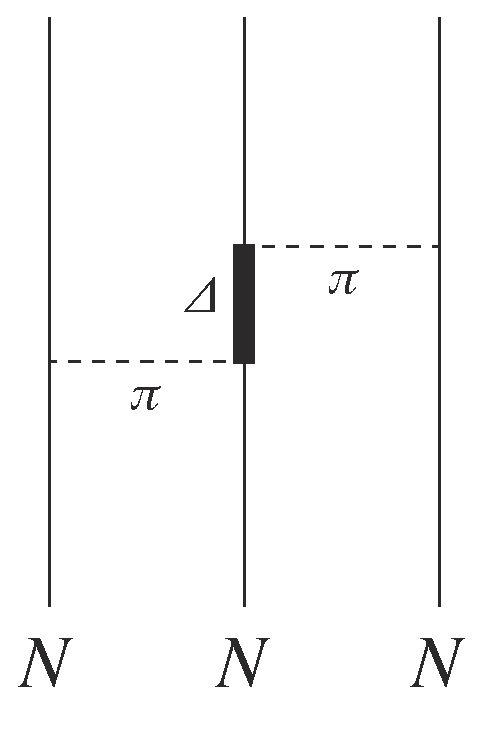
\includegraphics[clip,width=4cm]{./chap1/fig/3NF_2pi-model.pdf}\\
%  \caption{藤田-宮沢型三体核力モデルのFeynman図}
%  \label{FMmodel_FD}
% \end{figure}

% 現在用いられている主な三体核力のモデルとしてはUrbana IX\cite{Pud97}やTucson-Melbourne'99\cite{CH01}型がある。これらのモデルも藤田-宮沢型同様$2\pi$交換型の三体核力を主成分としたものである。

% %%%%%%%

% %% 1.2.2 %%
%   \subsection{散乱系における三体核力}
% 核力は運動量依存性およびスピン・アイソスピン依存性を持つ。よって、三体核力を含む核力の性質を詳細に調べる手段としては少数核子系散乱が非常に有効なプローブである。散乱実験によって三体核力の状態依存性を明確にすることは、その性質を調べていく上で重要である。\\
%  前述した二体核力の現実的な核力ポテンシャルおよび計算機の性能の向上により、近年では少数核子系の散乱における観測量について、モデルに依存しない厳密理論計算が可能となった。最も単純な三核子系散乱である核子--重陽子散乱については、低エネルギー領域において高精度の実験データとFaddeev方程式に基づく厳密理論計算との比較が行われた\cite{Glo96,KVR01}。その結果、核子当たり約30 MeV以下の低エネルギーではベクトル偏極分解能を除くほぼすべての観測量が二体核力のみを用いた計算で再現された。よって、低エネルギー領域においては三体核力の効果が二体核力に比べて非常に小さく、散乱実験によってその効果の寄与を観測することは困難であることが分かった。一方で、核子当たりの入射エネルギーがより大きくなると三体核力の効果も相対的に大きくなることが示唆された。\\
%  1998年には、Wita{\l}aらによって核子当たり約60 MeVにおける核子--重陽子散乱において三体核力の効果が現れることが理論的に初めて指摘された\cite{Wit98}。Wita{\l}aらの理論グループはTM型の三体核力モデルを含むFaddeev厳密理論計算を行い 、核子--重陽子弾性散乱における微分断面積が最小値を取る角度で三体核力の効果が顕著に現れることを示した。\\
%  理化学研究所のグループは、中間エネルギー領域での重陽子--陽子弾性散乱実験を行い、それによって得られた精緻な実験データから、理論的に予想された散乱系における三体核力の寄与大きさがほぼ正しいことを初めて明らかにした\cite{Sek02,Sek11}。例として、核子当たり135 MeVでの微分断面積の実験データおよび理論計算を図\ref{dcs_dp135}に示す。白丸が実験データ、青い帯が二体核力の核力ポテンシャル(AV18, CD-Bonn, Nijmegen I,II)のみを用いた理論計算であり、赤い帯が二体核力に三体核力(TM'99型)を入れ込んだ理論計算である。黒線は二体核力のAV18に三体核力であるUrbana IXを加えた理論計算である。理論計算による三体核力の寄与が重心系での散乱角度$\theta_{\rm c.m.} \sim 120^\circ$で現れている。この散乱角度では実験データが二体核力のみの理論計算よりも30%程度大きい値を取っているが、三体核力を考慮することで実験データを良く再現していることが分かる。

% \begin{figure}[tbp]
%  \centering
%  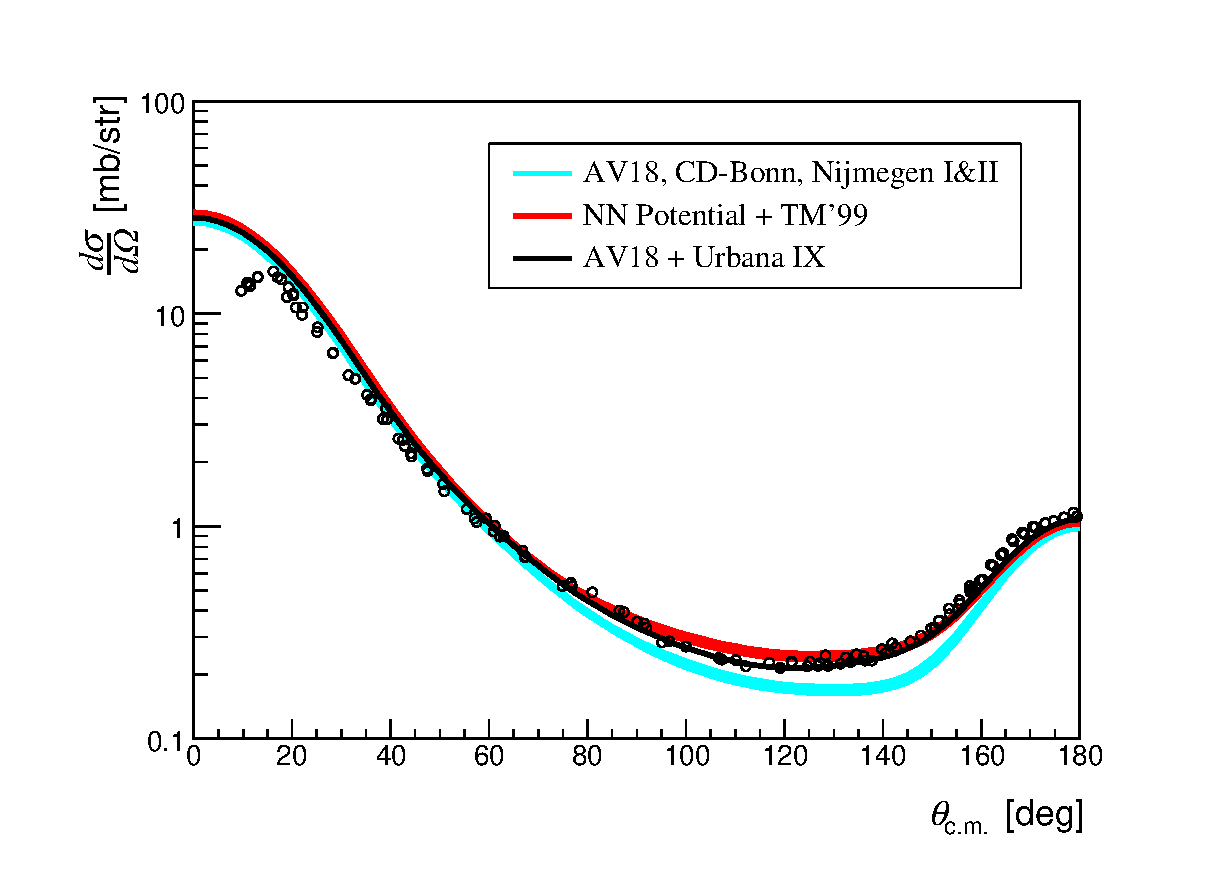
\includegraphics[clip,width=10cm]{./chap1/fig/dcs_dp_135MeV.eps}\\
%  \caption{核子当たり135 MeVでの重陽子--陽子弾性散乱の微分断面積\cite{Sek02}}
%  \label{dcs_dp135}
% \end{figure}

% %%%%%%%

% %% 1.2.3 %%
%   \subsection{四核子系散乱における三体核力}
% 近年では重陽子--陽子散乱のような三核子系だけでなく、四核子以上の核子系や、核物質の状態方程式においても三体核力の効果が重要視されている。例えば、質量数$A \sim 10$の軽い原子核の束縛エネルギーは、Green's Function Monte Carlo計算\cite{Pie01,PVW02}やNo-Core Shell Model計算\cite{NO03}などによって三体核力の効果を含んだ記述がなされており、その効果が無視できない大きさの寄与を与えるとされている。また中性子星の状態方程式においても三体核力による寄与が重要であることが示されており\cite{APR98}、中性子過剰な非対称核物質においては三体核力のアイソスピン依存性が重要となってくると示唆されている\cite{GCR12,Car15}。\\
%  我々のグループは、三体核力を含む核力から原子核という多体系を理論的に理解することを目指し、まず中間エネルギー領域における三体核力の性質を詳細に調べるため、実験プローブとして四核子である陽子--$^3$He散乱系を用いることにした。重陽子--陽子散乱では系のアイソスピンが$1/2$に限られているため、三体核力のアイソスピン依存性についてアプローチできない。しかし、陽子--$^3$Heのような四核子の散乱系では系のアイソスピンが$3/2$となるため、最終的には三体核力のアイソスピン依存性についてアプローチできると考えている。\\
%  陽子--$^3$Heの四核子散乱系については、Murdichらによって19.5 MeVから47.5 MeVの低エネルギー領域での弾性散乱における微分断面積が高精度で測定されている\cite{Mur84}。この測定による微分断面積はいずれも重陽子--陽子弾性散乱同様に$\theta_{\rm c.m.} \sim 120^\circ$で最小値を取っている。このことから中間エネルギー領域における陽子--$^3$He弾性散乱についても、微分断面積が最小値となる散乱角度において三体核力の効果を観測できると考えられる。\\
%  ここ数年では、三核子系だけでなく四核子の散乱系における観測量の厳密理論計算も可能になっている。およそ30 MeV以下での低エネルギー領域における陽子--$^3$He弾性散乱の観測量については、DeltuvaとFonseca\cite{DF13}やViviani\cite{Viv13}らによって理論計算が行われており、中間エネルギー領域において三体核力の効果が顕著に現れると予想されている。\\
%  中間エネルギー領域における陽子--$^3$Heの散乱系を系統的に調べていくために、まずこの散乱系の弾性散乱の完全測定を行うことを目標とした。完全測定とは、ある反応における散乱振幅のすべての要素が一意に決定できる測定である。このためには微分断面積だけでなく、偏極分解能などのスピン観測量の測定が必要不可欠である。偏極分解能とは反応に関わるいずれかの粒子がスピン偏極している時に観測される散乱の非対称を表す観測量である。偏極分解能の測定には、偏極ビームまたは偏極標的が必要となってくる。
  
% %%%%%%%

% %%%% 1.3 %%%%
%  \section{偏極${}^3$He標的}
% 前述のように我々のグループは、四核子系における三体核力の性質を詳細に調べていくために陽子--$^3$Heの散乱系の完全測定を目標とする。そのために、有効散乱角度における陽子--$^3$He弾性散乱での$^3$He偏極分解能測定を行う。我々は、この偏極分解能測定に必要不可欠である偏極$^3$He標的の開発を行ってきた。この節では、現在開発している偏極$^3$He標的に求められる条件および本研究以前の研究状況について述べる。

% %% 1.3.1 %%
%   \subsection{偏極$^3$He標的に要求される条件}
% 我々は測定によって得られた$^3$He偏極分解能の実験値と、理論計算によって得られた計算値とを比較することで、四核子系における三体核力の発現性について議論することを目的としている。そのためには高精度の実験データを得る必要がある。仮に$^3$He偏極分解能$A_y$をその統計誤差$dA_y$が0.02以下となるように測定することを要請した場合に、偏極標的に求められる条件について述べる。\\
%  陽子--偏極$^3$He弾性散乱における微分断面積は以下の式で与えられる。
% %
% \begin{equation}
%  \frac{d\sigma}{d\Omega} = \left( \frac{d\sigma}{d\Omega} \right)_0 ( 1+ {\bm p} \cdot {\bm A})
% \end{equation}
% %
% ここで$d\sigma/d\Omega$は$^3$He原子核が偏極している時の微分断面積で、添字の0は非偏極を表す。$\bm p$は$^3$He原子核の偏極度、$\bm A$はこの反応での$^3$He偏極分解能である。この式より、散乱角度$\theta$で散乱された陽子の検出数は、
% %
%  \begin{eqnarray}
%   L_{\rm up}=L_0[1+p_y A_y(\theta)] \\
%   L_{\rm down}=L_0[1-p_y A_y(\theta)] \\
%   R_{\rm up}=R_0[1-p_y A_y(\theta)] \\
%   R_{\rm down}=R_0[1+p_y A_y(\theta)]
%  \end{eqnarray}
%  %
% と表される。ここで、$L,R$ はビームの入射方向に対して左右に設置された検出器における散乱陽子の検出数である。左辺の添字は偏極方向の鉛直上向きおよび下向きを、右辺の0の添字は非偏極の場合を表す。またここでの座標系はマディソン規約\cite{Ohl72}に従い、ビームの入射軸を$z$軸、標的の偏極方向を散乱平面($xz$平面)に垂直な$y$軸に取っている(図\ref{madison}参照)。

% \begin{figure}[tbp]
%  \centering
%  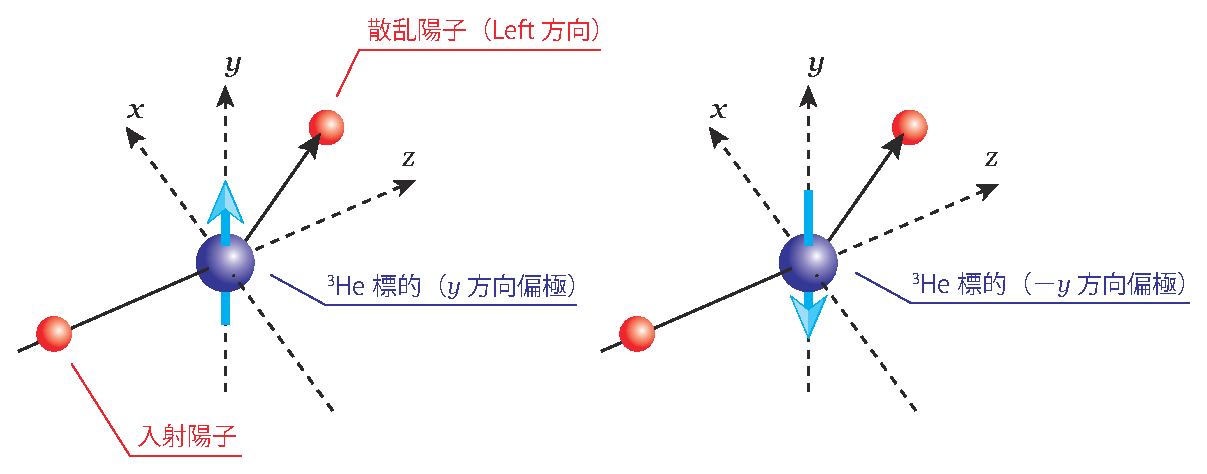
\includegraphics[clip,width=13cm]{./chap1/fig/madison.pdf}\\
%  \caption{マディソン規約から決定される陽子--偏極$^3$He散乱における座標系}
%  \label{madison}
% \end{figure}

% よって、これらの式から${}^3$Heの偏極分解能$A_y$は、次の式で求められる。
% %
%  \begin{equation}
%   A_y=\frac{1}{p_y} \frac{L_{\rm up}-L_{\rm down}}{L_{\rm up}+L_{\rm down}}=\frac{1}{p_y} \frac{R_{\rm down}-R_{\rm up}}{R_{\rm up}+R_{\rm down}}
%   \label{Ay_calc}
%  \end{equation}
%  %
% 偏極の向きを反転させれば、左右それぞれの検出器における反転前後の検出数の非対称度から偏極分解能を求めることができる。また偏極分解能の誤差$d A_y$は、次のように表される。
% %
%  \begin{eqnarray}
%   dA_y &=& \sqrt{\left( \frac{\partial A_y}{\partial Y_{\rm up}}\right)^2 (dY_{\rm up})^2+\left( \frac{\partial A_y}{\partial Y_{\rm down}}\right)^2 (dY_{\rm down})^2} \nonumber \\
%   (dA_y)^2 &=& \frac{1}{p_y^2} \frac{4}{(Y_{\rm up}+Y_{\rm down})^4}[Y_{\rm down}^2(dY_{\rm up})^2+Y_{\rm up}^2(dY_{\rm down})^2]
%   \label{Ay_err_1}
%  \end{eqnarray}
%  %
% ここで、左右の検出器において$dA_y$の表式は同じ形となるので、$Y=L,R$とした。$p_y A_y \ll 1$とすると、検出数の非対称度は小さくなるので、$Y \equiv Y_{\rm up} \sim Y_{\rm down}$となり、式(\ref{Ay_err_1})は
% %
%  \begin{equation}
%   (dA_y)^2 \sim \frac{1}{p_y^2} \frac{(dY)^2}{2Y^2}
%   \label{Ay_err_2}
%  \end{equation}
% %
% と近似できる。また検出器における粒子の検出数はPoisson分布に従うので、その統計誤差$dY_{\rm stat}$は$\sqrt{Y}$に等しくなる。よって式(\ref{Ay_err_2})は
% %
% \begin{equation}
%  (dA_y)^2 \sim \frac{1}{p_y^2} \frac{1}{2Y}
%  \label{Ay_err_3}
% \end{equation}
% %
% と表される。検出器における散乱粒子の検出数$Y$は次の式で表される。
% %
% \begin{eqnarray}
%  Y &=& N \cdot t \nonumber \\
%  &=& I \cdot \rho_{\rm T} \cdot \Delta \Omega \cdot \epsilon \cdot \frac{d\sigma}{d\Omega} \cdot t
%  \label{Yield}
% \end{eqnarray}
% %
% ここで$N$は単位時間あたりの散乱粒子の検出数、$t$は測定時間である。また$I$は入射粒子のフラックス、$\rho_{\rm T}$は標的粒子の単位面積あたりの数密度、$\Delta \Omega$は検出器の立体角、$\epsilon$は散乱粒子の検出効率で、$d\sigma/d\Omega$は微分断面積である。式(\ref{Yield})を式(\ref{Ay_err_3})に代入すると、$^3$He偏極分解能$A_y$の統計誤差は
% %
% \begin{equation}
%  (dA_y)^2 \sim \frac{1}{2p_y^2 \cdot \rho_{\rm T}} \frac{1}{I \cdot \Delta \Omega \cdot \epsilon \cdot \cfrac{d\sigma}{d\Omega} \cdot t}
%  \label{Ay_err_4}
% \end{equation}
% %
% となる。標的に関するパラメーターを見ると、$A_y$の統計誤差の2乗は標的粒子の単位面積あたりの数密度$\rho_{\rm T}$と標的の偏極度$p_y$の2乗の積に反比例する。よって、統計誤差を小さくするためには高密度かつ高偏極度の標的が必要となる。\\
%  次に、式(\ref{Ay_err_4})を用いて$^3$He偏極分解能の統計誤差$dA_y$が0.02以下となる時に要請される標的の条件を求める。標的以外(実験条件および測定系)に関するパラメーターについては、表\ref{para_Ay}のような値を仮定した。表\ref{para_Ay}の値を式(\ref{Ay_err_4})に代入すると、

% \begin{table}[htbp]
%  \caption{実験条件および測定系に関するパラメーターの仮定値}
%  \centering
%   \begin{tabular}{|c|c|} \hline
%   名称 & 仮定した値 \\ \hline \hline
%   測定時間 $t$ & 5時間 \\
%   ビーム強度 $I \cdot e$ & 5 nA \\
%   検出器の立体角 $\Delta \Omega$ & 0.5 msr \\
%   検出効率 $\epsilon$ & 100% \\
%   微分断面積 $d\sigma/d\Omega$ & 0.5 mb/sr \\ \hline
%   \end{tabular}
%  \label{para_Ay}
% \end{table}

% %
% \begin{eqnarray}
%  (dA_y)^2 &\sim& \frac{1}{2p_y^2 \cdot \rho_{\rm T}} \frac{1}{\cfrac{5 \times 10^{-9}}{1.6 \times 10^{-19}} \cdot 0.5 \times 10^{-3} \cdot 1 \cdot 0.5 \times 10^{-27} \cdot 5 \times 60^2} \nonumber \\
%   &\simeq& \frac{3.56 \times 10^{15}}{p_y^2 \cdot \rho_{\rm T}}
%   \label{Ay_err_5}
% \end{eqnarray}
% %
% となる。ここで、$^3$Heの原子量は3.015 g/molなので、標的の密度を$\rho~{\rm g/cm^3}$、長さを$l~{\rm cm}$とすると、
% %
% \begin{eqnarray}
%  (dA_y)^2 &\sim& \frac{3.56 \times 10^{15}}{p_y^2 \cdot \rho_{\rm T}} \nonumber \\
%  &=& \frac{3.56 \times 10^{15}}{p_y^2 \cdot \rho \cdot l \cdot \cfrac{6.022 \times 10^{23}}{3.015}} \nonumber \\
%  &\simeq& \frac{1.78 \times 10^{-8}}{p_y^2 \cdot \rho \cdot l}
%  \label{Ay_err_6}
% \end{eqnarray}
% %
% と計算できる。式(\ref{Ay_err_6})において、$dA_y<0.02$を要請すると、結局標的に求められる条件は次の式で表される。
% %
% \begin{equation}
%  p_y^2 \cdot \rho \cdot l > \frac{1.78 \times 10^{-8}}{(0.02)^2} = 4.45 \times 10^{-5}
%  \label{tar_cond}
% \end{equation}
% %
% $0$℃、$1$気圧における$^3$Heの密度は$1.35 \times 10^{-4}~{\rm g/cm^3}$であるから、$^3$Heガスの圧力を$3$気圧、標的の長さを$2~{\rm cm}$程度とすると、25%程度の偏極度が得られれば要請した統計誤差を満たす。\\
%  また式(\ref{Ay_calc})より、偏極分解能の値を求めるためには標的の偏極度が既知でなければならない。散乱実験が数十時間に渡って行われるものだとすれば、実験中に標的の偏極度を測定できるシステムが必要である。

% %%%%%%%

% %% 1.3.2 %%
%   \subsection{これまでの研究状況}
% 我々のグループは$^3$Heの偏極分解能の高精度測定のために、以上の条件を満たす偏極$^3$He標的の開発を行ってきた。これまでの開発で、$^3$Heガスを封入したガラスセルを作成し、スピン交換光ポンピング法による$^3$Heの偏極生成に成功している\cite{wada}。$^3$Heの偏極は、高速断熱通過-核磁気共鳴(AFP-NMR)法による測定を行うことで確認した。しかしAFP-NMR法による測定では$^3$He偏極度に対応した大きさの信号しか得られないので、偏極度の絶対値を求めることができない。そこでこの偏極$^3$He標的を用いて、$35~{\rm MeV}$の陽子ビームによる陽子--$^3$He弾性散乱実験を行った。$35~{\rm MeV}$での陽子--$^3$He弾性散乱における$^3$He偏極分解能はMcCamisらによって制度良く測定されており\cite{McC85}、この値から偏極度の絶対値を求めることができる。McCamisらによる$^3$He偏極分解能の測定結果を図\ref{Ay_35MeV}に示す。実験の結果、標的の偏極による散乱の非対称は観測されず、$^3$Heの偏極度が1%以下の非常に低い値であることが分かった。\\

% \begin{figure}[tbp]
%  \centering
%  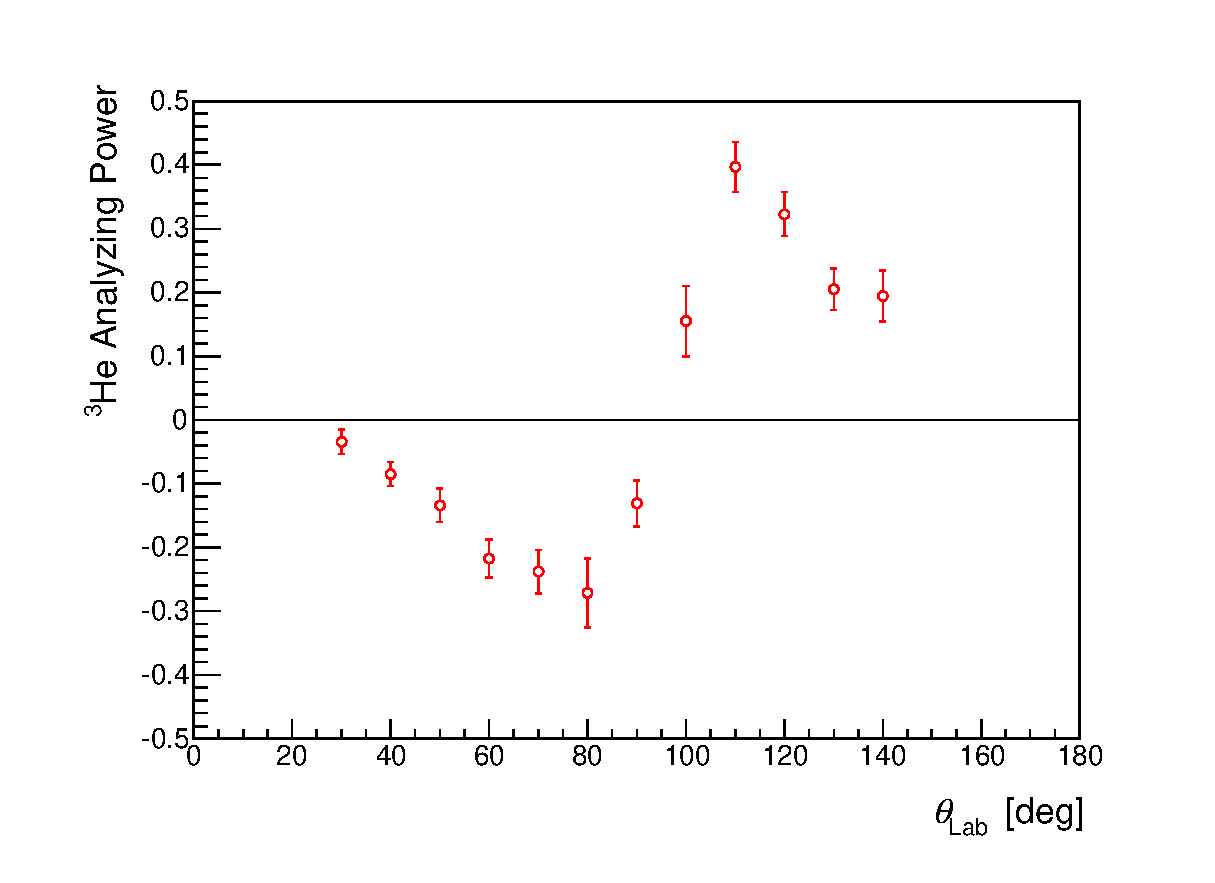
\includegraphics[clip,width=10cm]{./chap1/fig/Ay_p+3He_35MeV.eps}\\
%  \caption{$35~{\rm MeV}$の陽子--$^3$He弾性散乱における$^3$He偏極分解能\cite{McC85}}
%  \label{Ay_35MeV}
% \end{figure}

% これを受け、我々は$^3$He偏極度の向上のために偏極度シミュレーションによるガラスセルの最適化を行った\cite{shiokawa}。$^3$Heガスを封入するガラスセルの形状の最適化をすることで、効率よく光ポンピングを行い、結果的に$^3$He偏極度を向上させることを目的とした。これによって最適化されたガラスセルを新たに作成し、再び$35~{\rm MeV}$の陽子ビームによる陽子--$^3$He弾性散乱実験を行った。その結果、標的の偏極による散乱の非対称が観測された。しかし、同様に既知の$35~{\rm MeV}$での$^3$He偏極分解能から偏極度を求めた結果、およそ5%という値が得られ、要請された条件を満たしていないことが明らかとなった。

% %%%%%%%
% %%%%%%%%%%

% %%%% 1.4 %%%%
%  \section{本研究の目的}
% 以上のように、我々のグループが開発した偏極$^3$He標的は要請された条件を満たしておらず、偏極度の向上が必要である。また現在$^3$Heの偏極度を測定する方法として採用しているAFP-NMR法のみでは、偏極度の相対値しか求められない。現状では既知の$^3$He偏極分解能が得られている$35~{\rm MeV}$での陽子--$^3$He弾性散乱実験を行い、実験で得られた散乱の非対称から、標的の偏極度の絶対値を求める方法を取っている。しかしこの方法では偏極度の絶対値を得るために散乱実験を行わなければならず、また散乱の非対称は小さいので高精度で偏極度を得るのは困難である。最終的に中間エネルギー領域における$^3$He偏極分解能を高精度で得るためには、同様に高精度で$^3$He偏極度の絶対値を求める必要がある。偏極度の向上を目指すにあたっても容易に偏極度を測定できるシステムの構築が必要不可欠である。よって、本研究では新たな$^3$He偏極度測定システムを導入し、得られた偏極度からAFP-NMRの較正を行うことを目的とする。新たに導入する測定システムとして、Rbの電子スピン共鳴(ESR)を利用した$^3$He偏極度測定を採用した。また$^3$He偏極度の測定精度としては$10$%以下を目標とした。\\
%  以降の本稿の構成について簡潔に述べる。第2章では$^3$He原子核のスピン交換光ポンピング法による偏極生成の原理、またAFP-NMR法や本研究で導入するRbのESRを利用した$^3$He偏極度測定の原理について述べる。第3章では我々のグループにおける偏極$^3$He標的装置および標的製作装置について述べる。第4章では製作した標的を用いた偏極生成および新たに導入した$^3$He偏極度測定について述べる。第5章では東北大学サイクロトロンRIセンター(CYRIC)において行った$70~{\rm MeV}$の陽子ビームを用いた陽子--$^3$He弾性散乱実験について述べる。第6章では今回導入した$^3$He偏極度測定システムおよび偏極標的についての考察を述べ、第7章で本研究のまとめを述べる。

% %%%%%%%%%%

 \chapter{偏極陽子固体標的}
我々は、陽子の偏極生成手法として、光励起励起三重項電子スピンを用いた動的核偏極(Triplet-DNP)を用いている。
また、陽子偏極の偏極度測定方法として核磁気共鳴(NMR)を利用している。
本章では、まず陽子の偏極生成原理について説明し、その後NMRを利用した偏極の検出方法について述べる。

\section{偏極}
静磁場中の水素原子核スピン(I=1/2)は$|+1/2>, |-1/2>$いずれかのエネルギー固有状態となり、この各準位の占有数の偏りを偏極度という。
\begin{equation}
  P=\frac{N_+-N_-}{N_++N_-}
\end{equation}
一つのスピンの持つ磁化の大きさは
\begin{equation}
  \mu=\frac{1}{2}{\gamma_H} \hbar
\end{equation}
より、全体の磁化の大きさは
\begin{equation}
  M=N \mu P
\end{equation}
で表される。

\section{光励起励起三重項電子スピンを用いた動的核偏極(Triplet-DNP)の原理}
本研究では、偏極陽子標的としてナフタレンに重水素化ペンタセンを少量ドープした単結晶を用いている。
そして、ナフタレン内の水素原子核(陽子)の偏極生成手法として光励起励起三重項電子スピンを用いた動的核偏極(Triplet-DNP)を用いている。
この方法では、主に以下の3つの過程により陽子標的の偏極を行っている。

\begin{itemize}
  \item パルスレーザによる重水素化ペンタセン電子の偏極
  \item 電子スピンからナフタレン中の${}^1\rm{H}$スピンへの偏極移行
  \item 偏極拡散
\end{itemize}
本節では、この3つの過程に沿ってTriplet-DNPの基本原理について説明する。

\subsection{パルスレーザによる重水素化ペンタセン電子の偏極}
電子の偏極には、重水素化ペンタセンの光励起励起三重項電子スピン状態を利用している。
図$\ref{triplet_state}$に重水素化ペンタセンのエネルギー準位を示す。

\begin{figure}[tbp]
  \centering
  \includegraphics[clip,width=10cm]{./chap2/fig/triplet_state.png}\\
  \caption{重水素化ペンタセンのエネルギー準位図}
  \label{triplet_state}
\end{figure}

まず、600 nm以下の波長のパルスレーザの照射によって、基底状態($S_0$)から励起一重項状態($S_1$)へと重水素化ペンタセンの電子が励起される。
この$S_1$状態の電子は寿命$\sim 20$ nsで大半は基底状態($S_0$)に脱励起するが、わずかに$T_2$状態を経由して、最低次のスピン三重項状態である$T_1$状態に無放射的に脱励起するものが存在する。

このように、スピン多重度が異なる状態間の無放射遷移は項間交差(intersystem crossing)と呼ばれる。
これは禁制遷移だが、スピン軌道相互作用に起因する状態間の混合により生じる。\\
項間交差の選択性により、遷移する際に三重項状態の各準位間に占有数の差が生じる。
この占有数の差が電子の偏極である。

% 河原修論P6%
また、この占有数の差は外部磁場の方向と、重水素化ペンタセン分子の分子軸の間の角度によって変化する。
ここでペンタセン分子の分子軸と外磁場の向きを図$\ref{pentacene_axes}$に示すように定義すると、


\begin{figure}[ht]
  \centering
  \includegraphics[keepaspectratio, scale=0.5]
       {./chap2/fig/pentacene_axes.png}
  \caption{ペンタセン中のZFSテンソルの主軸系}
  \label{pentacene_axes}
 \end{figure}

 \begin{figure}[ht]
  \centering
  \includegraphics[keepaspectratio, scale=0.5]
       {./chap2/fig/energysplit_B0.png}
  \caption{ペンタセン分子軸と三重項副順位間の占有数の差$\cite{David}$}
  \label{energysplit}
 \end{figure}

 図$\ref{energysplit}$より、ペンタセン分子の長軸と外磁場が平衡であるときに各準位間の電子の占有数の差が
 最大になることがわかる。
 この時の三重項状態での占有数の割合はN(+1):N(0):N(-1)=12\%:76\%;12\%である$\cite{David}$。
偏極生成過程で用いるのは3つの副準位の占有数の差であるので、この2つの副準位だけを考える。この時、占有数の偏りの最大値は以下のように表される。
\begin{equation}
  \it P_{max}=\frac{\rm{N}(0)-\rm{N}(-1)}{\rm{N}(0)+\rm{N}(-1)}=\frac{\rm{76}(\%)-\rm{12}(\%)}{\rm{76}(\%)+\rm{12}(\%)}=\rm{73}(\%)
  \label{pentacene_P}
\end{equation}
この偏りは外磁場の方向とペンタセンの分子軸との間の角度だけに依存しており、外磁場の強さや温度には囚われないため高温、低磁場中でも$73\%$の電子偏極($P_e$)を得ることができる$\cite{David}$。
そして最後にこの$T_1$状態の電子は基底状態$S_0$に脱励起する。$T_1$状態では副順位間で寿命も異なる。
温度100 Kで報告されている値は$m_s=0$の時には$26 \mu sec$で、$m_s=\pm 1$の時には$83 \mu sec$である$\cite{Iinuma}$。

%丸田修論p20%
通常のペンタセンでも偏極は可能であるが、本研究では重水素化されたペンタセンを用
いている。これはペンタセンの代わりに重水素化ペンタセンを
ナフタレンにドープすることで、偏極度が向上することが確認されているからであ
る$\cite{Tateishi}$。ペンタセン中の ${}^1\rm{H}$ スピンは電子スピンが非常に近くに位置しているので、電子
スピンと強く結合し、電子${}^1\rm{H}$ 偏極交換の担い手になっている。しかし、同時に電子から
非常に強い緩和を受けているため、${}^1\rm{H}$ スピンの緩和時間を押し下げている。そこで、重
水素化ペンタセンを用いることでこの緩和を抑制し、偏極度を向上させることができる。
なおこれにより偏極交換は、遠くにある(結合強度の小さい)ナフタレン中の ${}^1\rm{H}$ ス
ピンと行わなければならなくなるが、ICP パラメータの調整次第で、通常のペンタセンと
ほぼ同等の効率で偏極交換ができる。

\subsection{電子スピンから${}^1\rm{H}$スピンへの偏極移行}
電子スピンと ${}^1\rm{H}$ スピン間の偏極交換には、Integrated Corss Polarization 法 (ICP)
と呼ばれる方法を用いる。この方法では、以下の式$\ref{Hartmann-Hahn}$を満たすとき、電子スピンの高
偏極状態が  ${}^1\rm{H}$スピンへと移行される。

\begin{equation}
  \omega_{eff e}=\omega_{0 H}
  \label{Hartmann-Hahn}
\end{equation}

ここで$\omega_0 H$は${}^1\rm{H}$スピンのラーモア周波数、$\omega_{eff e}=\sqrt{\omega^2_{1e}+\Delta\omega^2_e}$は電子スピンの実効磁場強度で、$\omega_{1e}$は電子スピンのラビ周波数、$\Delta\omega_e$はオフセット周波数である。
つまり、電子スピンの実効的なラビ周波数と ${}^1\rm{H}$ スピンのラーモア周波数を一致させるこ
とが偏極移行のための条件であり、式 $\ref{Hartmann-Hahn}$ は Hartmann-Hahn 条件と呼ばれる。この
Hartmann-Hahn 条件を満たした時、電子スピンと ${}^1\rm{H}$ スピンの超微細結合ハミルトニア
ンがフリップフロップ項を持ち、電子スピンの偏極が ${}^1\rm{H}$ スピンへ移行
される。しかし、電子スピンの共鳴周波数は、核スピンとの超微細結合によって不均一に
広がっている(図$\ref{spin_packet}$)。そのため、個々のスピンパケットが感じる実行磁場はそれぞれ異
なり、マイクロ波を電子スピンに照射しても一部の電子しか Hartmann-Hahn 条件を満
たすことができない。この問題は、Henstra の静磁場を掃引するというアイディアにより
解決された$\cite{Henstra1}$。

\begin{figure}[ht]
  \centering
  \includegraphics[keepaspectratio, scale=0.5]
       {./chap2/fig/spin_packet.png}
  \caption{電子スピンパケットの拡がりと電子スピン共鳴の磁場掃引}
  \label{spin_packet}
 \end{figure}

 この方法では、図$\ref{spin_packet}$のように、電子スピンの共鳴周波数が、
 照射するマイクロ波周波数よりも低くなる磁場から高くなる磁場まで掃引する。Henstra らはこの
 方法を Integrated Solid Effect(ISE) と名付けた$\cite{Henstra2}$。磁場掃引を含めた ICP のシー
 クエンスを図$\ref{pulse_sequence}$に示す。

 \begin{figure}[ht]
  \centering
  \includegraphics[keepaspectratio, scale=1.5]
       {./chap2/fig/pulse_sequence.png}
  \caption{ICPシークエンス}
  \label{pulse_sequence}
 \end{figure}

 磁場掃引を中心磁場 $B_0$、掃引幅 $B_S$ で、$\tau_S$ の間行う場合、磁場の時間変化 $B_0(t)$ は以
 下の式$\ref{B0t}$のように書ける。

\begin{equation}
  B_0(t)= B_0 \pm \frac{B_S}{\tau_S}(t-\frac{\tau_S}{2})
  \label{B0t}
\end{equation} 

磁場の掃引が以下の式$\ref{Insulation conditions}$で表される断熱条件を満たすときに、電子スピンパケットは
実効磁場の方向にロックされていく [44]。

\begin{equation}
  \gamma_e\frac{dB_0(t)}{dt} \ll \frac{\omega^2_e}{\rm{sin}\alpha(t)}
  \label{Insulation conditions}
\end{equation}

ここで$\alpha (t)$は、静磁場と実効磁場のなす角である。磁場の掃引方向を変えることで、正
偏極生成と負偏極生成を変えることができる。

\subsection{スピン拡散}
${}^1H$ スピンが数多く存在している系の回転座標系のハミルトニアンは、以下の式$\ref{Hamiltonian}$のように書ける。

\begin{equation}
  \mathcal{H}_{II}={\displaystyle \Sigma_{j,k}}d_{j,k}[2I_{jz}I_{kz}-\frac{1}{2}(I_{j+}I_{k-}+I_{j-}I_{k+})]
  \label{Hamiltonian}
\end{equation}

$I_j$ は j 番目の I スピンのスピン演算子で、$d_{j,k}$ は j 番目と k 番目の I スピン間の双極子
相互作用の結合定数である。$d_{j,k}(I_j+I_k− + I_{j−}I_{k+})/2$ はフリップフロップ項であり、お
互いのスピンの z 成分を交換させる働きがある。全ての I スピン間で偏
極率の交換が行われているため、物質中で偏極率に空間的偏りがある場合には、この交換
によってその空間的偏りはならされていく。この熱拡散のような現象はスピン拡散と呼ば
れている。

\subsection{Triplet-DNPによる偏極の蓄積}
ICP 後、三重項状態は無放射遷移で、元の基底一重項状態 $S_0$ へと戻る。重水素化ペン
タセン近傍に局在する ${}^1H$ スピンの高偏極状態はスピン拡散により周囲のホスト分子の
${}^1H$ スピンへ移っていく。ペンタセン近傍の高偏極状態が標的サンプル全体に拡散した後、
再びパルスレーザによる光励起、マイクロ波照射による ICP を行えば、さらに高偏極状
態を積み重ねることができる。この過程を何度も繰り返していくことで、${}^1H$ スピンに高
偏極状態を蓄積することができる。
飯沼・武田らは、Triplet-DNP による ${}^1H$ スピン偏極率 P の上昇の様子を、偏極生成
時定数 ${T_D}$ とレーザ照射時の偏極緩和時定数 $T_{1laser}$ を用いて、以下の式のような
レート方程式で表現できることを示した$\cite{Takeda}$。

\begin{equation}
  \frac{dP}{dt}=\frac{1}{T_D}(P_e-P)-\frac{1}{T_{1laser}}(P-P_{th})
  \label{pol_dif}
\end{equation}
ここで、$P_e$ は電子スピンの偏極率、$P_{th}$ は ${}^1H$ スピンの熱平衡状態の偏極率である。ま
た、$T_{1laser}$ は ${}^1H$ スピンのスピン-格子緩和時間 $T_1$ と、${}^1H$ スピンとの偏極交換に使われ
なかった残留偏極電子による緩和 $T_e$ を用いて以下の式$\ref{T_{1laser}}$のように表せる。

\begin{equation}
  \frac{1}{T_{1laser}}=\frac{1}{T_1}+\frac{1}{T_e}
  \label{T_{1laser}}
\end{equation}

本実験条件では $P_{th}$ は非常に小さいため、$P_{th}$ を無視して式を解くと以下の解$\ref{pol}$を得る。

\begin{equation}
  P(t)=\frac{P_e}{1+\frac{T_D}{T_{1laser}}}\left[1-exp\left(-\left(\frac{1}{T_D}+\frac{1}{T_{1laser}}\right)\right)t\right]
  \label{pol}
\end{equation}


\section{陽子の偏極信号の検出}
陽子の偏極信号の検出には、NMR 法を利用する。

\subsection{NMRの基本原理}
\subsubsection{ゼーマン相互作用}
スピンIはZ軸方向にかけられた静磁場$\textbf{B}_0 = (0, 0, B_0)$ 中で、式$\ref{Zeeman}$のゼーマン相
互作用によってエネルギー分裂が生じる。

\begin{equation}
  \mathcal{H}_{Zeeman}=-\gamma B_0 I_Z=\omega_{0I}I_Z
  \label{Zeeman}
\end{equation}


ここで、$\gamma$ は磁気回転比、$\omega_{0I}$ はラーモア周波数である。またスピン演算子 $\textbf{I} = (I_x , I_y , I_z)$
は、パウリ行列:

\begin{equation}
  \textbf{1}=
  \begin{pmatrix}
    1 & 0 \\
    0 & 1 \\
  \end{pmatrix}
  ,
  \sigma_x=
  \begin{pmatrix}
    0 & 1 \\
    1 & 0 \\
  \end{pmatrix}
  ,
  \sigma_y=
  \begin{pmatrix}
    0 & -i \\
    i & 0 \\
  \end{pmatrix}
  ,
  \sigma_z=
  \begin{pmatrix}
    1 & 0 \\
    0 & -1 \\
  \end{pmatrix}
  \label{pauli_matrix}
\end{equation}
を用いて式$\ref{spin_operator}$で表される。
\begin{equation}
  I_x=\frac{\sigma_x}{2},
  I_y=\frac{\sigma_y}{2},
  I_z=\frac{\sigma_z}{2}
  \label{spin_operator}
\end{equation}
さらに、スピン昇降演算子$I_+,I_-$を以下の式$\ref{spin_updown}$で定義する。
\begin{equation}
  I_+=I_x+iI_y=
  \begin{pmatrix}
    0 & 1 \\
    0 & 0 \\
  \end{pmatrix}
  ,I_-=I_x-iI_y=
  \begin{pmatrix}
    0 & 0 \\
    1 & 0 \\
  \end{pmatrix}
\label{spin_updown}
\end{equation}

\subsubsection{密度演算子と回転座標系}
現実的な多粒子状態を考える場合、全ての粒子状態について一つ一つ記述することは不
可能である。そこで、以下の式で定義される密度演算子を導入する。
\begin{align}
\begin{aligned}
  \hat{\rho} &= \mathbb{N}^{-1}(\ket{\psi_1}\bra{\psi_1}+\ket{\psi_2}\bra{\psi_2}+\dots)\\
            &= \overline{\ket{\psi} \bra{\psi}}
\end{aligned}
\end{align}
スピン状態の密度演算子 $\rho$ の時間発展は、リウビル-フォンノイマン方程式$\ref{Liouville}$で記述できる。

\begin{equation}
  \frac{d}{dt}\rho(t)=i[\rho(t),\mathcal{H}]
  \label{Liouville}
\end{equation}
ハミルトニアンが時間依存しない時は、以下の式$\ref{Liouville2}$で状態の時間発展が記述できる。

\begin{align}
  \begin{aligned}
    \rho(t)&=&U\rho(0)U^{-1}\\
          U&=&\rm{exp}(-i\mathcal{H}t)
    \label{Liouville2}
  \end{aligned}
\end{align}

NMR によるスピンダイナミクスを理解しやすくするために、Z 軸まわりに $\omega I$ で回転
する回転座標系を導入する。回転座標系から見たスピン状態 $\rho^R$は、以下の式$\ref{rhoR}$で与えられる。

\begin{align}
  \begin{aligned}
  \rho^R(t)&=U(t)^{-1}\rho(t)U(t)\\
  U(t)&=\rm{exp}(-i\omega_I I_Z t)
  \label{rhoR}
  \end{aligned}
\end{align}
したがって、回転座標系のハミルトニアンは式$\ref{Hamiltonian_R}$のように与えられる。

\begin{equation}
  \mathcal{H}^R = U(t)^{-1}\mathcal{H}^R U(t)-iU(t)^{-1}\frac{d}{dt}U(t)
  \label{Hamiltonian_R}
\end{equation}

\subsubsection{双極子相互作用}
2 スピン($\textbf{I}$スピン、$\textbf{S}$スピン)間には双極子相互作用が働く。実験室座標系における
双極子相互作用のハミルトニアンは、以下の式$\ref{dipole_H}$で与えられる。

\begin{align}
  \begin{aligned}
    \mathcal{H}_{IS}&=b_{IS}\left[\frac{3(\textbf{I}\cdot \textbf{r}_{IS})(\textbf{S}\cdot \textbf{r}_{IS})}{r^2_{IS}}-\textbf{I}\cdot \textbf{S} \right]\\
    b_{IS}&=-\frac{\mu_0}{4\pi}\frac{\gamma_I \gamma_S \hbar}{r^3_{IS}}
    \label{dipole_H}
  \end{aligned}
\end{align}

ここで、$r_{IS}$ は核間ベクトル、$r_{IS}$ は核間ベクトルの長さ、$\mu_0$ は真空の透磁率、$\gamma_I\gamma_S$ は
$\textbf{I},\textbf{S}$ スピンの磁気回転比を表す。式$\ref{dipole_H}$の双極子相互作用ハミルトニアンは、以下の
式$\ref{dipole_H2}$で書き直すことができる$\cite{Abragam}$。


\begin{align}
  \begin{aligned}
    \mathcal{H}_{IS}&=b_{IS}(A+B+C+D+E+F)\\
    A&=(3cos^2\theta_{IS}-1)I_ZS_Z\\
    B&=-\frac{1}{4}(3cos^2\theta_{IS}-1)(I_+S_-+I_-S_+)\\
    C&=\frac{3}{2}sin\theta_{IS}cos\theta_{IS}e^{-i\phi}(I_+S_Z+I_ZS_+)\\
    D&=\frac{3}{2}sin\theta_{IS}cos\theta_{IS}e^{-i\phi}(I_-S_Z+I_ZS_-)\\
    E&=\frac{3}{4}sin^2\theta_{IS}e^{-2i\phi}I_+S_+\\
    F&=\frac{3}{4}sin^2\theta_{IS}e^{2i\phi}I_-S_-\\
    \label{dipole_H2}
  \end{aligned}
\end{align}
ここで $\theta_{IS}$ は Z 軸と核間ベクトルのなす角度である。静磁場下では、系のハミルトニア
ンは以下の式$\ref{H_Z}$のように書ける。

\begin{equation}
  \mathcal{H}=\omega_{0I}I_Z+\omega_{0S}S_Z
  \label{H_Z}
\end{equation}

ここで $\omega_{0I} , \omega_{0S}$ はそれぞれ I スピンと S スピンのラーモア周波数である。I スピンが
$\omega_{0I}$ で、S スピンが $\omega_{0S}$ でそれぞれ回転する座標系、すなわち二重回転座標系における系
のハミルトニアンは、以下の式 (B.13) で与えられる。

\begin{equation}
  siki
\end{equation}

$|\omega_{0I}-\omega_{0S}|\gg b_{IS}$  場合、すなわち異種核間の場合、$\omega_{0I} I_Z + \omega_{0S}S_Z$ は式$\ref{dipole_H2}$で示
される A とは可換で、その他の項とは非可換となる。この非可換な項の時間発展は平均
化され、ほとんど状態発展に寄与しないと考えて良い。よって、異核間双極子相互作用は
以下の式$\ref{H_DR}$のようになる。

\begin{equation}
  siki
  \label{H_DR}
\end{equation}

これをセキュラー近似(secular approximation)と呼ぶ$\cite{Levitt}$。
$\omega_{0I}=\omega_{0S}$場合、すなわち同核間の場合、$ \omega_{0I}(I_Z + S_Z) $は式$\ref{dipole_H2}$で示される A, B
とは可換で、その他の項とは非可換となる。よって、同核間双極子相互作用は、以下の式$\ref{H_DR2}$で与えられる。

\begin{equation}
  \label{H_DR2}
\end{equation}

式$\ref{H_DR2}$の$\frac{1}{2}(I_+S_− + I_−S_+)$ はフリップフロップ項と呼ばれている。初期状態$P_I I_Z +P_SS_Z +\frac{1}{4}$ の 2 スピン系にこのフリップフロップ項を$ \frac{\pi}{d_{IS}}$
秒間作用させると、以下の式$\ref{UFF1}$のように、I スピンと S の Z 成分を交換する。
\begin{equation}
  siki
  \label{UFF1}
\end{equation}
\begin{equation}
  siki
  \label{UFF2}
\end{equation}
すなわち、フリップフロップ項を作用させることは、偏極率を交換することに対応する。

\subsubsection{RF照射と自己誘導減衰}
Z軸方向の静磁場$B_0$下で、X軸方向のラジオ波(RF)磁場$B_{1I}(t)= - \frac{2\omega_{1I}}{\gamma_I}cos(\omega_It+\phi_I)$
照射下での、実験室座標系における I スピンのハミルトニアンは、以下の式$\ref{RF_H}$で与えられる。

\begin{equation}
  siki
  \label{RF_H}
\end{equation}

$\omega_I$はRF照射のキャリア周波数、$\phi_I$は初期位相である。$\omega_{1I}$はラビ周波数である。式
$\ref{RF_H}$で示したハミルトニアンを回転座標系において書き直すと、以下の式$\ref{RF_H2}$のようになる。

\begin{equation}
  siki
  \label{RF_H2}
\end{equation}

この時、回転波近似を用いた。
$\omega_{0I} = \omega_I$ のオンレゾナンス照射の場合、照射位相$\phi_I=0^\circ$で X 軸回りの$\theta$回転となる。

\begin{equation}
  siki
  \label{RX}
\end{equation}

RF 照射により得られる NMR 信号は量子力学的には、$I_-$ 演算子の期待値で表される。
\begin{equation}
  Tr[\rho I_-]
  \label{Tr}
\end{equation}
1 スピン系の場合、初期状態 $\rho_0 =\frac{1}{2}+P_{thI}I_z$ のスピンに $\frac{\pi}{2}$ パルスを作用させると、
以下の式$\ref{rho_2}$のようになる。

\begin{equation}
  siki
  \label{rho_2}
\end{equation}

その後の状態は、以下の式$\ref{rho_3}$のように書き表される。

b\begin{equation}
  siki
  \label{rho_3}
\end{equation}

ここでは、$\omega_0$ は核スピンのラーモア周波数で、$T_2$ はスピン-スピン緩和時間を示してい
る。この時、$I_-$ 演算子の期待値は、以下の式$\ref{Tr2}$のようになる。

\begin{equation}
  siki
  \label{Tr2}
\end{equation}

これが得られる NMR 信号であり、自由誘導減衰(Free Induction Decay: FID)と呼ぶ

\subsection{偏極度モニター}
偏極発展・緩和中の陽子偏極度は、NMR 測定系によって常にモニターしている。RF
照射によって磁化を倒すことで、偏極による磁化の大きさの相対値がわかるが、${\frac{\pi}{2}}_x$ パ
ルスを照射した場合、標的結晶内のスピン偏極は全て破壊されてしまう。そこで、偏極度
モニターを行う場合は、RF 照射によるフリップ角を小さく設定する。そうすることで、
磁化の大きさ M に対して、$Msin\theta$ の FID 信号を観測しつつ、$M(1 − cos \theta)$ の偏極状態
を残すことができる(図 2.9)。
本研究において、フリップ角は $\theta =12^{\circ}$ に設定した。この時、磁化の大きさ M に対して約
21$\%$ の強度の FID 信号を観測しつつ、1 回の NMR 測定による減偏極は $1-cos \theta \sim 2.2\%$
となる。ナフタレン偏極陽子標的の場合、20分に 1 回程度の測定間隔であればこの減
偏極は元に戻る。このように、フリップ角を小さく設定することで、高い偏極を維持した
まま偏極度のモニターを行うことができる。



\section{偏極生成および測定装置}
\subsection{電磁石}
本研究では、有限会社タカノ技研製の電磁石を使用した$\ref{magnet}$。コイルの形状や
磁極間の隙間(185 mm)を工夫することで、散乱実験における広角度測定(±60◦)を可
能にしながら、最大 0.329 T の磁場が印加できるように設計されている。$\ref{magnet}$(b) は、製
作時の 80 A の電流を印加した時の水平面内の磁場強度分布である。また、$\ref{magnet}$(c) は、
90 A の電流を印加した時の x 軸方向の磁場強度分布である。ここで、標的結晶の中心を
原点としており、座標軸は$\ref{magnet}$(a) に示すように z 軸はビームの進行方向に対応する。
標的結晶サイズの範囲における磁場の不均一度は $\leq0.1\%$ を達成した。HIMAC における
ビーム照射試験では、電流を 79.3 A 印加し、磁場強度を 0.299 T に設定した。

\begin{figure}[ht]
  \centering
  \includegraphics[keepaspectratio, scale=0.8]
       {./chap2/fig/magnet.png}
  \caption{(a)実際の電磁石の写真。(b)80 Aの電流印加時の水平面の磁場強度分布。(c)90 Aの電流印加時のx軸方向の磁場強度分布。標的結晶の中印を原点とする。座標軸はz軸をビームの進行方向としている。標的結晶サイズの範囲における磁場の不均一度は$\leq0.1\%$である。}
  \label{magnet}
 \end{figure}

\subsection{標的チェンバー}
$\ref{chamber_str}$に標的結晶周辺のシステムを示す。標的結晶はテフロン製のサンプルホルダーに
装着し、マイクロ波を効率的に標的に照射するための TE011 型共振器の中心に設置した。
共振器には磁場掃引用のコイルと NMR 測定用のコイルが取り付けられている。また、標
的結晶の角度調整を行うために歯車を用いた回転システムを導入している。
図$\ref{chamber}$に標的チェンバーの模式図を示す。図に示す黒の点線の位置に図$\ref{chamber_str}$のシステム
が導入されている。ナフタレン標的の昇華を防ぐために液体窒素による冷却を行い、冷却による霜
の発生を防止するために真空を引く必要があるため、チェンバーを二重構造とした。


\begin{figure}[ht]
  \centering
  \includegraphics[keepaspectratio, scale=0.8]
       {./chap2/fig/chamber_str.png}
  \caption{標的結晶周辺のシステムの模式図}
  \label{chamber_str}
 \end{figure}

 \begin{figure}[ht]
  \centering
  \includegraphics[keepaspectratio, scale=0.5]
       {./chap2/fig/chamber.png}
  \caption{標的チャンバーの模式図。黒の点線内に図$\ref{chamber_str}$のシステムが導入されている}
  \label{chamber}
 \end{figure}

\subsection{パルスレーザ}
パルスレーザは、株式会社 Changchun New Industries Optoelectronics Technology
製の LD 励起固体レーザ(HPL-556-Q-5mJ)を使用した。このレーザは、波長 556 nm、
パルス幅約 600 ns に設定され、最大 5 mJ の単一パルスを発生させることができ、10 Hz
∼ 4 kHz までの繰り返し動作が可能になっている。HIMAC におけるビーム照射試験で
は、パルスの出力を 5 mJ、繰り返し周波数を 1.5 kHz に設定した。図 3.9 に示すように
レーザ光は、加速器実験におけるビームとの干渉を避けるために、標的チェンバーの上流
側に取り付けられた 2 箇所の光学窓から照射される。また、レーザ光の一部はフォトダイ
オードに照射し、TTL 信号に変換してマイクロ波照射と磁場掃引のトリガーに使用した。

\subsection{磁場掃引・マイクロ波回路}
レーザ光をトリガーとし、磁場掃引およびマイクロ波の照射を行うようにした。磁場掃引は、ファンク
ションジェネレーター(NF 社、WF1943A)を用いて三角波(5 Vpp)を生成し、オペア
ンプで増幅後マイクロ波共振器内のコイルに入力した。
マイクロ波は RF オシレータ(SynthHD, Windfreak Tech., LLC)で生成した。そ
の後ファンクションジェネレータ(F.G.)からレーザ光をトリガーとした矩形波を単
極単投(SPST)スイッチに送り、スイッチを制御することでマイクロ波パルスを整形
した。パルス化されたマイクロ波は、RF パワーアンプ(株式会社アールアンドケー、
CA9000BW1G-5060RP)で 400 W まで増幅し、TE011 型共振器へ送った。図$\ref{circuit}$に
Triplet-DNP システムの回路図を示す。

\begin{figure}[ht]
  \centering
  \includegraphics[keepaspectratio, scale=0.8]
       {./chap2/fig/circuit.png}
  \caption{Triplet-DNPシステムの回路図}
  \label{circuit}
 \end{figure}

 \subsection{NMR測定装置}
 NMR 装置の簡潔な回路図を図$\ref{duplexer}$に示す。RF の照射および FID 信号の検出は、デュ
 プレクサを介することで同じ NMR コイルにて行われる。また、NMR 観測シーケンスの
 作成や NMR 信号の受信は OPENCORE NMR 分光計$\cite{Takeda2} $で行っている。回路の共振
 は、チューナーボックス内の可変コンデンサで調節した。

\begin{figure}[ht]
  \centering
  \includegraphics[keepaspectratio, scale=1.0]
       {./chap2/fig/duplexer.png}
  \caption{NMR装置の回路図}
  \label{duplexer}
 \end{figure}


\section{HIMACにおける偏極陽子標的のビーム照射試験}
量子科学技術研究開発機構 HIMAC において、ナフタレン偏極標的に対
して 200 MeV の陽子ビームの照射試験を行った。十分偏極発展が飽和した偏極標的に対
して陽子ビームを照射し、定期的に NMR 測定によって偏極度をモニターすることで放
射損の評価を行った。図 4.6 に 200 MeV の陽子ビーム照射時のナフタレン標的の
NMR 信号強度(FID 信号をフーリエ変換後積分した値)を示す。
この測定では、$1\times10^6$cps のビーム強度で 2 回照射を行い、1 回目では 7.5 h、2 回目
では 10 h 照射した。また 20 分に 1 回の頻度でフリップ角を 12◦ に設定した NMR 測定
を行なった。グラフ$\ref{HIMAC_data}$では、ビーム照射直前の NMR
信号強度を 1 としている。赤色のエリアはビーム照射時であることを示している。
\begin{figure}[ht]
  \centering
  \includegraphics[keepaspectratio, scale=0.7]
       {./chap2/fig/HIMAC_data.png}
  \caption{200 MeV陽子ビーム照射時のナフタレン標的のNMR信号強度。ビーム照射直前のNMR信号強度を1とした。赤色の領域はビーム照射時を示している。}
  \label{HIMAC_data}
 \end{figure}

 グラフ$\ref{HIMAC_data}$に示すようにビーム照射時には偏極度が徐々に低下する
 ことが確認された。

 



% 我々は陽子--$^3$He弾性散乱による$^3$He偏極分解能測定のために、偏極$^3$He標的の開発を行ってきた。この章では、$^3$He原子核の偏極方法とその偏極度の測定方法について記述する。$^3$He原子核の偏極方法としては、スピン交換光ポンピング(Spin Exchange Optical Pumping, SEOP)法を採用した。

% %%%% 2.1 %%%%
%  \section{偏極標的}
% 陽子や中性子の偏極標的は核子のスピン構造の研究に必要不可欠なものである。しかし、陽子に対して自由空間中の中性子は不安定であり、およそ15分の寿命で陽子に$\beta$崩壊してしまう。標的として使用するためには高密度かつ安定である必要があり、現状ではそのような大量の中性子を分離し安定させることは不可能である。偏極中性子標的として原子核物理学や素粒子物理学等において広く開発、利用されているのが偏極$^3$He標的である。$^3$He原子核は2個の陽子と1個の中性子から成り、Pauli原理から陽子はスピン一重項状態となるので、その磁気モーメントは互いに打ち消し合う。よって、$^3$He原子核の正味の磁気モーメントは中性子の磁気モーメントとほぼ等しくなる。また$^3$He原子核の核スピンのおよそ$90$%が中性子のスピンによる寄与であることが示されており\cite{Fri90}、偏極中性子標的として偏極$^3$He標的を実験的に用いることができる。また$^3$He原子核は低エネルギーの中性子に対して、スピンの向きに依存した吸収断面積を持っている\cite{Cou88}。$^3$He原子核スピンと反平行のスピンを持つ中性子に対して大きい吸収断面積を示すので、中性子を偏極させるための偏極子\cite{Cou90}や、偏極した中性子の偏極度計\cite{GTD95}としても利用されている。

% %%%%%%%%%%

% %%%% 2.2 %%%%
%  \section{$^3$He原子核の偏極方法}
% $^3$He原子核を偏極させる方法としては主に二つある。ひとつは準安定交換法(Metastability Exchange Optical Pumping, MEOP)\cite{CSW63}と呼ばれる方法である。これは高周波の放電によって$^3$He原子の電子スピンを$2{}^3S_1$の準安定状態に励起させ、これに1083 nmの円偏光を照射することで$2{}^3P_0$の励起準位へと遷移させる。これによって電子スピンをZeeman分裂した$2{}^3S_1$の特定の副準位へと占有させ、電子スピンを偏極させることができる。この電子スピン偏極は更に基底状態の$^3$He原子核との超微細相互作用によって原子核スピンへと移され、結果的に${}^3$He原子核を偏極させることができる。この反応の断面積は$\sim 10^{-16} \ {\rm cm^2}$と非常に大きいので、高い偏極度を実現できる。しかし、高周波の放電を保持するために$^3$Heガスの圧力を低くする必要があり、およそ数 Torrに制限される。本研究では3気圧程度の$^3$Heガスを想定しているので、この方法は本研究に不適である。\\
%  二つ目は本研究でも採用しているSEOP法\cite{BCV60}である。散乱実験等で必要な高密度の偏極$^3$He標的を実現できるのは現状ではこの方法だけである。SEOP法は主に二つの過程によって$^3$He原子核を偏極させる。最初に、Rb蒸気に円偏光レーザーを照射することでRb原子を偏極させる(光ポンピング)。次に、$^3$He原子核とのスピン交換相互作用によってRb原子の偏極を$^3$He原子核へ移行させる。これらの過程を経て、$^3$He原子核を偏極させる。光ポンピングに数十 W程度の高出力レーザーを用いれば、高密度の$^3$Heガスで高偏極度を実現できる。近年では、$5$気圧程度の圧力で$60$%以上の偏極度が得られている\cite{Ye10}。\\
%  以上より、本研究では$^3$He原子核を偏極させる方法としてSEOP法を採用した。以下の節ではこのSEOP法の原理および高速断熱通過-核磁気共鳴(Adiabatic Fast Passage Nuclear Magnetic Resonance, AFP-NMR)法とRbの電子スピン共鳴(Electron Spin Resonance, ESR)測定による$^3$He原子核の偏極度測定原理について述べる。
% %\textcolor{red}{未}

% %%%%%%%%%%

% %%%% 2.3 %%%%
%  \section{スピン交換光ポンピング法}
%  前述のように、SEOP法は円偏光レーザーによってアルカリ金属原子を偏極させ(光ポンピング)、その偏極した原子と$^3$He原子核とが超微細相互作用(Hyper Fine Interaction, HFI)をすることによってスピン交換が起こり、$^3$He原子核を偏極させる二段階の過程で行う方法である。この節ではこのSEOP法による$^3$He原子核の偏極原理についてそれぞれの過程に分けて述べる。一般的に、光ポンピングにはRb原子が用いられるが、K原子やNa原子、およびそれらの混合蒸気を用いる方法もある\cite{Bab03, Bor03}。本研究では、偏極させるアルカリ金属原子にはRb原子を採用した。

% %% 2.3.1 %%
%   \subsection{光ポンピングによるRb原子の偏極}
%   Rbの同位体は主に$^{85}$Rbと$^{87}$Rbの二種類があり、それらの天然存在比はそれぞれ$72.17%, 27.83%$である。$^{85}$Rbの核スピンは$I=5/2$であり、電子スピンを$S=1/2$、電子の軌道角運動量を$L$、電子の全角運動量を$J=L+S$とすると、Rb原子の全角運動量$F$は$|I-J| \le F \le I+J$の値を取りうる。またそれぞれの$F$の状態は磁気量子数$m_F$について縮退しており、静磁場をかけることによってZeeman分裂する。$^{85}$Rb原子のエネルギー準位を図\ref{85Rb_ene}に示す。
  
% \begin{figure}[tbp]
%  \centering
%  \includegraphics[clip,width=9cm]{./chap2/fig/85Rb_ene_mf.pdf}\\
%  \caption{$^{85}$Rbのエネルギー準位}
%  \label{85Rb_ene}
% \end{figure}
  
%   アルカリ金属原子の偏極には、光子を吸収または放出する際の角運動量選択則を利用している。Rb原子の$D_1$遷移波長(795 nm)の光を入射すると共鳴が起き、Rb原子は$5{}^2S_{1/2}$から$5{}^2P_{1/2}$へと励起する。またこの時、静磁場によってRb原子の準位がZeeman分裂している状態で磁場と平行な右回りの円偏光($\sigma_+$)を入射すると、角運動量選択則により$\Delta m_J=+1$の遷移のみが起こる。よって、$5{}^2S_{1/2}$の準位にいるRb原子の価電子のうち$m_J=-1/2$の準位にいたものだけが$5{}^2P_{1/2}$の$m_J=+1/2$の準位へと選択的に励起される。またこの励起したRb原子は、他の原子が存在しない場合においては$5{}^2S_{1/2}$の$m_J=-1/2$または$m_J=+1/2$状態に脱励起する。この脱励起が起こる確率はClebsch-Gordan係数に従い、それぞれ$2/3, 1/3$となる。この様子を示したのが図\ref{85Rb_ene_pump}である。図ではRb原子の核スピンの影響を無視して簡略化したエネルギー準位を示している。実際にはRb原子の他に最終的に偏極させる3気圧程度の$^3$Heガスや、$\rm N_2$ガスも同時に封入させる。これらの“バッファガス”を混在させると、Rb原子との衝突によって$5{}^2P_{1/2}$の二つの準位($m_J= \pm 1/2$)が混合し(collisional mixing)、$5{}^2S_{1/2}$の二つの準位へとそれぞれ1/2の同確率で脱励起するようになる。円偏光を絶えず入射させれば$5{}^2P_{1/2}$へ励起され続けるので、光子の吸収と脱励起を繰り返し、$5{}^2S_{1/2}$の$m_J=+1/2$状態が占有され、Rb原子を偏極させることができる。
  
% \begin{figure}[tbp]
%  \centering
%  \includegraphics[clip,width=9cm]{./chap2/fig/85Rb_seop.pdf}\\
%  \caption{核スピンの影響を無視した$^{85}$Rbのエネルギー準位および光ポンピングの模式図}
%  \label{85Rb_ene_pump}
% \end{figure}
  
% Rb原子が脱励起する時にも光子が放出される。$m_J=+1/2$状態から$m_J=-1/2$状態への脱励起の場合は右回りの円偏光($\sigma_+$)、$m_J=-1/2$状態から$m_J=+1/2$状態への脱励起の場合は左回りの円偏光($\sigma_-$)の光子が放出され、同じ磁気量子数間での脱励起の場合は非偏光($\pi$)の光子が放出される。脱励起によって放出された光子を吸収することでもRb原子が励起する(radiation trapping)ため、$5{}^2S_{1/2}$の$m_J=+1/2$状態にいるRb原子も励起されてしまい、結果的にRb原子の偏極を飽和させる要因となる。この現象を防ぐために、バッファガスとして$\rm N_2$ガスを封入する。バッファガスを含んだ場合の光ポンピングの模式図を図\ref{85Rb_ene_buf}に示す。円偏光によって励起したRb原子は、$\rm N_2$分子との衝突によってそのエネルギーを$\rm N_2$分子の振動や回転のエネルギーとして渡し、脱励起する。このことによって、光子を放出することなく脱励起させることができる。このとき励起したRb原子が光子を放出して脱励起する確率$B_{\gamma}$は、$\rm N_2$ガスの分圧を$P_{\rm N_2}$とすると、
% %
% \begin{equation}
%  B_{\gamma}=\frac{3}{3+P_{\rm N_2}}
% \end{equation}
% %
% と表される\cite{WC89}。加えられる$\rm N_2$ガスの典型的な分圧は$100 \ \rm Torr$程度であり、このとき光子の放出を伴う遷移が起こる確率はおよそ$3$%にまで抑制される。
  
% \begin{figure}[tbp]
%  \centering
%  \includegraphics[clip,width=9cm]{./chap2/fig/85Rb_seop2.pdf}\\
%  \caption{バッファガス($\rm N_2$)を含んだ場合での光ポンピングの模式図}
%  \label{85Rb_ene_buf}
% \end{figure}

% 次に、以上の条件下におけるRb原子の偏極度の表式を求める。Rb原子の偏極度を$P_{\rm Rb}$とすると、
% %
% \begin{equation}
%  P_{\rm Rb}=\frac{\rho_+ - \rho_-}{\rho_+ + \rho_-}=\rho_+ - \rho_-
%  \label{P_Rb}
% \end{equation}
% %
% となる。$\rho_{\pm}$はRb原子の$m_J= \pm 1/2$における占有確率で、$\rho_+ + \rho_-=1$である。占有確率$\rho_{\pm}$の時間変化は次のように表される\cite{Lar91}。
% %
% \begin{equation}
%  \frac{d\rho_{\pm}(x)}{dt} = \pm \left( \gamma_{\nu}^+(x)+\gamma_{\nu}^0(x)+\Gamma_{\rm Rb}-D\frac{d^2}{dx^2} \right)\rho_-(x) \mp \left( \frac{\Gamma_{\rm Rb}}{2}+\frac{\gamma_{\nu}^0(x)}{2} \right)
%  \label{rho_Rb}
% \end{equation}
% %
% ここで、$\gamma_{\nu}^{+, 0}(x)$は位置$x$での円偏光($\sigma_+$)および直線偏光の光子がRb原子に吸収される割合で、$\Gamma_{\rm Rb}$はRb原子の偏極緩和率、$D$は$^3$Heガス中でのRb原子に対する有効拡散定数で、ガスが封入されているセルの境界付近でのRb原子の偏極度およびガスの非一様性の効果を表している。レーザー光が完全に円偏光している場合は$\gamma_{\nu}^0(x)=0$である。またガスが十分高圧、高密度であれば占有確率$\rho_{\pm}(x)$はセル内でほぼ一様と考えられるので、
% %
%  \begin{equation}
%   -D \frac{d^2}{dx^2} \rho_-(x) \ll 1
%  \end{equation}
% %
% と近似できる。よって式(\ref{rho_Rb})は以下のように単純化される。
% %
% \begin{eqnarray}
%  \frac{d\rho_{\pm}(x)}{dt} & = & \pm \left( \gamma_{\nu}^+(x)+\Gamma_{\rm Rb} \right) \rho_-(x) \mp \frac{\Gamma_{\rm Rb}}{2} \nonumber \\
%  & = & \pm \left( \gamma_{\nu}^+(x)+ \frac{\Gamma_{\rm Rb}}{2} \right) \rho_-(x) \mp \frac{\Gamma_{\rm Rb}}{2}\rho_+(x)
%  \label{drho/dt}
% \end{eqnarray}
% %
% 式(\ref{P_Rb}), (\ref{drho/dt})より、Rb原子の偏極度$P_{\rm Rb}$の時間変化は次のように表される。
% %
% \begin{eqnarray}
%  \frac{dP_{\rm Rb}(x)}{dt} & = & \frac{d}{dt}(\rho_+(x)-\rho_-(x)) \nonumber \\
%  & = & -\left( \gamma_{\nu}^+(x)+\Gamma_{\rm Rb} \right) P_{\rm Rb}(x)+\gamma_{\nu}^+(x)
% \end{eqnarray}
% %
% この微分方程式を解くと、結局Rb原子の偏極度は
% %
% \begin{equation}
%  P_{\rm Rb}(x, t) = \left( \frac{\gamma_{\nu}^+(x)}{\gamma_{\nu}^+(x)+\Gamma_{\rm Rb}} \right) \left[ 1-e^{-(\gamma_{\nu}^+(x)+\Gamma_{\rm Rb})t} \right]
%  \label{P_Rb_xt}
% \end{equation}
% %
% と書ける。十分な時間円偏光による光ポンピングを行い平衡状態に達したと仮定すると、この時のRb原子の偏極度$\overline{P}_{\rm Rb}$は、式(\ref{P_Rb_xt})の$t \to \infty$の極限を取って
% %
% \begin{equation}
%  \overline{P}_{\rm Rb}(x) = \frac{\gamma_{\nu}^+(x)}{\gamma_{\nu}^+(x)+\Gamma_{\rm Rb}}
%  \label{P_Rb_ave}
% \end{equation}
% %
% となる。すなわち、Rb原子の偏極度は光ポンピングによる円偏光($\sigma^+$)の光子の吸収率$\gamma_{\nu}^+(x)$とRb原子の偏極緩和率$\Gamma_{\rm Rb}$の比で表される。\\
%  円偏光($\sigma^+$)の光子の吸収率$\gamma_{\nu}^+(x)$は次のように表される。
% %
% \begin{equation}
%  \gamma_{\nu}^+(x) = \int \Phi(x, \nu) \sigma_{\rm abs}(\nu) d\nu
%  \label{gam+}
% \end{equation}
% %
% ここで$\Phi(x, \nu)$は位置$x$における単位周波数あたりの円偏光($\sigma^+$)光子の光束であり、$\sigma_{\rm abs}(\nu)$は周波数$\nu$の光子に対する吸収断面積である。\\
%  光子はRb蒸気中を進むにつれ吸収され数が減少していくため、円偏光光子の光束$\Phi(x, \nu)$は$x$方向に対して以下のような関係を持つ。
% %
% \begin{eqnarray}
%  \Phi(0, \nu) &=& \frac{I_{\rm laser}(\nu)}{h\nu} \\
%  \frac{d\Phi(x, \nu)}{dx} &=& -[{\rm Rb}] \sigma_{\rm abs}(\nu) (1-P_{\rm Rb}(x)) \Phi(x, \nu)
% \end{eqnarray}
% %
% ここで、$I_{\rm laser}(\nu)$は円偏光レーザーの単位周波数および単位面積あたりの出力で、$h$はPlanck定数である。\\
%  吸収断面積$\sigma_{\rm abs}(\nu)$は次の式で表される\cite{Lar91}。
% %
% \begin{equation}
%  \sigma_{\rm abs}(\nu) = \frac{\lambda_0^2}{8\pi}\Gamma_{\rm nat} \left[ \frac{\Gamma}{(\nu-\nu_0)^2+(\Gamma/2)^2}+\frac{b(\nu-\nu_0)}{\Gamma} e^{-\frac{|\nu-\nu_0|}{\Gamma_a}} \right]
%  \label{sig_abs}
% \end{equation}
% %
% ここで$\lambda_0=794.979~{\rm nm}$、$\nu_0=c/\lambda_0$はそれぞれRb原子の$D_1$遷移波長および周波数であり、$\Gamma_{\rm nat}=5.75~{\rm MHz}$は自然線幅である。$\Gamma$はバッファガスによる全圧力拡がり幅で、$b$および$\Gamma_a$は観測された吸収スペクトルの非対称を説明するための補正係数である。これらの値はLarsonらによって測定されており、それぞれの値は表\ref{par_abs}のようになる。またバッファガスとして$2.94$気圧の$^3$Heガスが存在する時のRb原子の光子吸収断面積$\sigma_{\rm abs}$を図\ref{sig_abs_Rb}に示す。

% \begin{table}[htbp]
%  \caption{Rbの$D_1$線遷移に対する光子吸収の係数\cite{Lar91}}
%  \centering
%  \begin{tabular}{|c|ccc|} \hline
%   $^3$He圧力 [atm] & $\Gamma$ [GHz] & $\Gamma_a$ [GHz] & $b$ [$10^{-12}$ s] \\ \hline \hline
%   2.94 & $54 \pm 3$ & $154 \pm 11$ & $0.20 \pm 0.04$ \\
%   6.44 & $126 \pm 5$ & $146 \pm 11$ & $1.0 \pm 0.2$ \\ 
%   8.97 & $184 \pm 6$ & $184 \pm 11$ & $1.5 \pm 0.2$ \\
%   12.1 & $244 \pm 7$ & $225 \pm 12$ & $1.5 \pm 0.2$ \\ \hline
%  \end{tabular}
%  \label{par_abs}
% \end{table}

% \begin{figure}[tbp]
%  \centering
%  \includegraphics[clip,width=10cm]{./chap2/fig/sigma_abs.eps}\\
%  \caption{Rb原子の$D_1$遷移の光子吸収断面積}
%  \label{sig_abs_Rb}
% \end{figure}

% 次に、Rb原子の偏極緩和率$\Gamma_{\rm Rb}$の表式を求める。Rb原子の偏極緩和の主な要因は、Rb原子と他の原子が衝突することによって起こるスピン-回転相互作用である\cite{WWH85}。このスピン-回転相互作用のハミルトニアンは以下のように書ける。
% %
% \begin{equation}
%  \mathcal{H}_{\rm SR} = \gamma {\bm N} \cdot {\bm S}
% \end{equation}
% %
% ここで$\gamma$は結合定数、$\bm N$は衝突した二つの粒子による回転運動の角運動量ベクトルであり、$\bm S$はRb原子の価電子スピンである。一般的に、光ポンピングに用いられる混合気体にはRb、$^3$HeおよびN$_2$が含まれるので、偏極したRb原子は主にこれらの原子との相互作用によって緩和する。よって、Rb原子の偏極緩和率$\Gamma_{\rm Rb}$は混合気体中の各原子の数密度に比例し、次の式で表される\cite{Lar91,WC94}。
% %
% \begin{equation}
%  \Gamma_{\rm Rb} = \langle \sigma_{\rm SD} v \rangle [{\rm Rb}]+\langle \sigma_{\rm N_2} v \rangle [{\rm N_2}]+\langle \sigma_{\rm SE} v \rangle [^3{\rm He}]+k_3 [^3{\rm He}]^2
%  \label{relax_Rb}
% \end{equation}
% %
% ここで、$\langle \sigma v \rangle$は二粒子間の反応断面積$\sigma$および相対速度$v$の積を速度分布で平均化した反応率である。$\sigma_{\rm SD}$はRb同士での反応断面積で、$\sigma_{\rm N_2}$はRb-N$_2$間、$\sigma_{\rm SE}$はRb-$^3$He間での反応断面積である。$k_3$はRbと二つの$^3$Heによる三体衝突における反応率である。また式中の[ ]は各原子または分子の数密度を表す。各反応率はWagshulとChupp\cite{WC94}やLarsonら\cite{Lar91}によって求められており、それぞれの値は以下のようになる。
% %
% \begin{eqnarray}
%  \langle \sigma_{\rm SD} v \rangle &=& (8.3 \pm 0.6) \times 10^{-13}~[{\rm cm^3/s}] \\
%  \langle \sigma_{\rm N_2} v \rangle &=& (9.38 \pm 0.22) \times 10^{-18}~[{\rm cm^3/s}] \\
%  \langle \sigma_{\rm SE} v \rangle &=& (6.1 \pm 0.2) \times 10^{-20}~[{\rm cm^3/s}] \\
%  k_3 &\sim& 7.48 \times 10^{-39}~[{\rm cm^6/s}]
% \end{eqnarray}
% %
% これらの値から、Rb原子の偏極緩和率$\Gamma_{\rm Rb}$を概算する。$^3$Heの密度は$0~℃$、$1$気圧下で$1.35 \times 10^{-4}~{\rm g/cm^3}$であり、$^3$He原子の原子量は$3.015~{\rm g/mol}$である。またN$_2$分子の密度は$0~℃$、$1$気圧下で$1.25 \times 10^{-3}~{\rm g/cm^3}$であり、またN$_2$分子の分子量は$28.01~{\rm g/mol}$である。$^3$Heガスの圧力を$3$気圧、N$_2$ガスの圧力を$100~{\rm Torr}$とすると、それぞれの数密度は室温($300~{\rm K}$)においては
% %
% \begin{eqnarray}
%  [^3{\rm He}] &\simeq& 7.36 \times 10^{19}~[{\rm cm^{-3}}]
%  \label{[3He]} \\
%  {[{\rm N_2}]} &\simeq& 3.20 \times 10^{18}~[{\rm cm^{-3}}]
%  \label{[N2]}
% \end{eqnarray}
% %
% となる。またRb原子の数密度については、Killianによって温度に対するRbの飽和蒸気圧が測定されており\cite{Kil26}、絶対温度$T$におけるRb原子の飽和密度は
% %
% \begin{equation}
%  [{\rm Rb}] = 10^{26.41-\frac{4132}{T}-\log_{10}T}~[{\rm cm^{-3}}]
%  \label{Killian_eq}
% \end{equation}
% %
% と表される。式(\ref{Killian_eq})より、$200$℃におけるRb原子の数密度は
% %
% \begin{equation}
%  [{\rm Rb}] \simeq 10.05 \times 10^{14}~[{\rm cm^{-3}}]
% \end{equation}
% %
% と求められる。よって、以上の条件下におけるRb原子の偏極緩和率$\Gamma_{\rm Rb}$は、式(\ref{relax_Rb})にこれらの値を代入して
% %
% \begin{equation}
%  \Gamma_{\rm Rb} \simeq 909~[{\rm s^{-1}}]
% \end{equation}
% %
% となる。
% %%%%%%%

% %% 2.3.2 %%
%   \subsection{スピン交換による$^3$He原子核の偏極}
% Rb蒸気と$^3$Heガスが混在した空間では、Rb原子の価電子と$^3$He原子核の間で超微細相互作用(HFI)が起こり、それによってRb原子の偏極が$^3$He原子核へと移行する(スピン交換)。HFIによるスピン交換の概念図を図\ref{spin_exch}に示す。Rb原子の価電子と$^3$He原子核とのHFIにおけるハミルトニアンは次の式で表される\cite{Her65}。
% %
% \begin{equation}
%  \mathcal{H}_{\rm HFI} = -2 \gamma_{\rm ^3He} \mu_{\rm N} \mu_{\rm B} \sum_{i=1}^3 \left[ \frac{{\bm I} \cdot {\bm J}_i}{r_i^3} - 3\frac{({\bm I} \cdot {\bm r}_i)({\bm J}_i \cdot {\bm r}_i)}{r_i^5} - \frac{8\pi}{3} \delta({\bm r}_i) {\bm I} \cdot {\bm J}_i \right]
% \end{equation}
% %
% ここで、$\gamma_{\rm ^3He}$は$^3$Heの磁気回転比であり、$\mu_{\rm N}$は核磁気モーメント、$\mu_{\rm B}$はBohr磁子である。$\bm I$は$^3$He原子核の核スピンで、${\bm J}_i$は$i$番目の電子のスピンである。${\bm r}_i$は$^3$He原子核から見た$i$番目の電子に対する位置ベクトルであり、$i=1$はRb原子の価電子、$i=2,3$は$^3$Heの電子を表す。また$ \delta({\bm r}_i)$は三次元デルタ関数である。括弧内の第一項および第二項は二粒子間での磁気双極子相互作用を表し、第三項はFermi接触相互作用を表す項である。

% \begin{figure}[tbp]
%  \centering
%   \includegraphics[width=9cm]{./chap2/fig/spin_exchange.pdf}\\
%  \caption{Rb原子と$^3$He原子核のスピン交換反応の概念図}
%  \label{spin_exch}
% \end{figure}

% 次に、$^3$He原子核の偏極度の表式を求める。静磁場中の$^3$He原子核はRb原子と同様に磁気量子数$m_I=\pm 1/2$についてZeeman分裂する。この分裂した二つの副準位それぞれの占有確率を$\tilde{\rho}_{\pm}~(\tilde{\rho}_+ + \tilde{\rho}_- =1)$とすると、$^3$He原子核の偏極度は
% %
% \begin{equation}
%  P_{\rm ^3He} = \frac{\tilde{\rho}_+ - \tilde{\rho}_-}{\tilde{\rho}_+ + \tilde{\rho}_-} = \tilde{\rho}_+ - \tilde{\rho}_-
%  \label{P_3He}
% \end{equation}
% %
% と表される。占有確率$\tilde{\rho}_{\pm}$の時間変化は次の式で表される\cite{Lar91}。
% %
% \begin{equation}
%  \frac{d\tilde{\rho}_{\pm}}{dt} = \pm \left( \frac{\Gamma_{\rm ^3He}}{2} + \gamma_{\rm SE}\rho_+ \right) \tilde{\rho}_- \mp \left( \frac{\Gamma_{\rm ^3He}}{2} + \gamma_{\rm SE}\rho_- \right) \tilde{\rho}_+
%  \label{drho/dt_3He}
% \end{equation}
% %
% ここで、$\gamma_{\rm SE}$はRb原子と$^3$He原子核のスピン交換率で、$\Gamma_{\rm ^3He}$は$^3$He原子核の偏極緩和率である。スピン交換率$\gamma_{\rm SE}$はRb原子の数密度に比例し、
% %
% \begin{equation}
%  \gamma_{\rm SE} = \langle  \sigma_{\rm SE} v \rangle [{\rm Rb}] \equiv k_{\rm SE} [{\rm Rb}]
% \end{equation}
% %
% と書ける。$k_{\rm SE}$はスピン交換率係数であり、Larsonら\cite{Lar91}やChannら\cite{Cha02}によって測定されている。それぞれの値は$(6.1 \pm 0.2) \times 10^{-20}~{\rm cm^3/s}$ \cite{Lar91}, $(6.8 \pm 0.2) \times 10^{-20}~{\rm cm^3/s}$ \cite{Cha02}と求められている。\\
%  $\tilde{\rho}_+ + \tilde{\rho}_- =1$より、式(\ref{drho/dt_3He})を整理すると、結局$^3$He偏極度の時間変化は次のように表される。
% %
% \begin{equation}
%  \frac{dP_{\rm ^3He}}{dt} = -(\gamma_{\rm SE}+\Gamma_{\rm ^3He}) P_{\rm ^3He} + \gamma_{\rm SE} \overline{P}_{\rm Rb}
%  \label{dP_3He/dt}
% \end{equation}
% %
% ここで、Rb原子の偏極度$P_{\rm Rb}$は$^3$He原子核の偏極度$P_{\rm ^3He}$に比べて十分早く平衡状態に達すると仮定し、$\overline{P}_{\rm Rb} \sim \rho_+ - \rho_-$とした。式(\ref{dP_3He/dt})を解くと、結局$^3$He原子核の偏極度$P_{\rm ^3He}$は以下の式で表される。
% %
% \begin{equation}
%  {P}_{\rm ^3He} = \overline{P}_{\rm Rb} \frac{\gamma_{\rm SE}}{\gamma_{\rm SE}+\Gamma_{\rm ^3He}} \left[ 1-e^{-(\gamma_{\rm SE}+\Gamma_{\rm ^3He})t} \right]
%  \label{P_3He_final}
% \end{equation}
% %
% 式(\ref{P_3He_final})より、十分時間が経過した時($t \to \infty$)の$^3$He原子核の偏極度$\overline{P}_{\rm ^3He}$は
% %
% \begin{equation}
%  \overline{P}_{\rm ^3He} = \overline{P}_{\rm Rb} \frac{\gamma_{\rm SE}}{\gamma_{\rm SE}+\Gamma_{\rm ^3He}}
%  \label{P_3He_ave}
% \end{equation}
% %
% と表される。また式(\ref{P_Rb_ave})より
% %
% \begin{equation}
%  \overline{P}_{\rm ^3He} = \frac{\gamma_{\nu}^+(x)}{\gamma_{\nu}^+(x)+\Gamma_{\rm Rb}} \frac{\gamma_{\rm SE}}{\gamma_{\rm SE}+\Gamma_{\rm ^3He}}
%  \label{P_3He_ave2}
% \end{equation}
% %
% となる。よって、$^3$He原子核の偏極度を向上させるためには、円偏光光子の吸収率$\gamma_{\nu}^+$をなるべく大きくしつつ、Rb原子の偏極緩和率$\Gamma_{\rm Rb}$を小さくすることでRb原子の偏極度$\overline{P}_{\rm Rb}$を向上させることが必要である。またスピン交換率$\gamma_{\rm SE}$をなるべく大きくしつつ、$^3$He原子核の偏極緩和率$\Gamma_{\rm ^3He}$を小さくすることも必要である。これらのパラメーターはRb原子の数密度$[{\rm Rb}]$に依存し、また$[{\rm Rb}]$は式(\ref{Killian_eq})より温度依存性を持つので、$^3$He原子核の偏極度を向上させるためにはRb蒸気の温度を最適化することが重要である。\\
%  次に、$^3$He原子核の偏極緩和率$\Gamma_{\rm ^3He}$について述べる。$^3$He原子核の偏極緩和の原因は主に以下の3つである。
% %
% \begin{enumerate}
%  \item $^3$He原子核同士の磁気双極子相互作用による緩和($\Gamma_D$)
%  \item 静磁場の不均一度による緩和($\Gamma_B$)
%  \item ガラスセル内に含まれる不純物やセルの内壁との接触による緩和($\Gamma_W$)
% \end{enumerate}
% %
% $^3$He原子核の偏極緩和率$\Gamma_{\rm ^3He}$はこれらの和で表される。以下に、それぞれの緩和の原因について述べる。\\
%  $^3$He原子核同士の磁気双極子相互作用による偏極緩和率$\Gamma_D$は、Newburyらによって計算されており、
% %
% \begin{equation}
%  \Gamma_D = \frac{[{\rm ^3He}]}{744}~[{\rm h}^{-1}]
% \end{equation}
% %
% と表される\cite{New93}。ここで、$^3$Heの数密度$[{\rm ^3He}]$の単位はamagat($1 {\rm amg} = 2.689 \times 10^{19}~{\rm cm^{-3}}$)である。$3$気圧、$300~{\rm K}$の$^3$Heガスを仮定すると、式(\ref{[3He]})より$[{\rm ^3He}]$はamagat単位において
% %
% \begin{equation}
%  [{\rm ^3He}] = \frac{7.36 \times 10^{19}}{2.689 \times 10^{19}} \simeq 2.74~[{\rm amg}]
% \end{equation}
% %
% となる。よって、$\Gamma_D$は
% %
% \begin{equation}
%  \Gamma_D = \frac{2.74}{744} \simeq 3.68 \times 10^{-3}~[{\rm h^{-1}}]
%  \label{Gam_D}
% \end{equation}
% %
% と計算できる。\\
%  静磁場の不均一度による偏極緩和率$\Gamma_B$は次の式で表される\cite{CSH88}。
% %
% \begin{equation}
%  \Gamma_B = D_{\rm ^3He} \frac{|\nabla B_x|^2+|\nabla B_y|^2}{B_z^2}
%  \label{Gam_B}
% \end{equation}
% %
% ここで、$D_{\rm ^3He}$は偏極した$^3$He核スピンの拡散定数であり、$B_x,~B_y,~B_z$は静磁場の各軸成分である。偏極した$^3$He核スピンの拡散定数$D_{\rm ^3He}$は、GamblinとCarverによって次の式で表されることが示されている\cite{GC65}。
% %
% \begin{equation}
%  D_{\rm ^3He} = \frac{1}{2.13} \frac{\lambda v}{(1+ \omega^2 \tau^2)}
%  \label{D_3He}
% \end{equation}
% %
% ここで、$\lambda$および$v$は$^3$He原子の平均自由行程と二乗平均速度($\sqrt{\langle v^2 \rangle}$)である。また$\omega$は$^3$He核スピンのLarmor歳差運動周波数で、$\tau = \lambda/v$は$^3$Heガスの衝突時間である。圧力$p$、温度$T$の気体における平均自由行程$\lambda$は、次のように書ける。
% %
% \begin{equation}
%  \lambda = \frac{k_{\rm B}T}{\sqrt{2} \sigma p}
%  \label{MFP}
% \end{equation}
% %
% ここで、$k_{\rm B}$はBoltzmann定数であり、$\sigma$は気体粒子の幾何学的断面積である。気体粒子が半径$r$の剛体球だとすれば$\sigma = 4 \pi r^2$と書けるので、半径$r$としてHeのVan der Waals半径($1.40~$\AA)を用いると、結局$3$気圧、$300~{\rm K}$の$^3$Heガスにおける平均自由行程$\lambda$は
% %
% \begin{eqnarray}
%  \lambda &=& \frac{1.38 \times 10^{-23} \cdot 300}{\sqrt{2} \cdot 4 \pi \cdot (1.40 \times 10^{-10})^2 \cdot 3 \times 1.013 \times 10^5} \nonumber \\
%  &\simeq& 3.91 \times 10^{-8}~[{\rm m}]
%  \label{MFP_cal}
% \end{eqnarray}
% %
% となる。二乗平均速度$v$は、気体粒子がMaxwellの速度分布に従っているとすると、
% %
% \begin{equation}
%  v = \left( \frac{3k_{\rm B}T}{m} \right)^{\frac{1}{2}}
%  \label{MSV}
% \end{equation}
% %
% と書ける。$^3$He原子の質量は$2809~{\rm MeV}$なので、$3$気圧、$300~{\rm K}$の$^3$Heガスにおける二乗平均速度$v$は
% %
% \begin{eqnarray}
%  v &=& \left( \frac{3 \cdot 1.38 \times 10^{-23} \cdot 300}{2809 \times 10^6 \div (3.0 \times 10^8)^2 \cdot 1.6 \times 10^{-19}} \right)^{\frac{1}{2}} \nonumber \\
%  &\simeq& 1.58 \times 10^3~[{\rm m/s}]
%  \label{MSV_cal}
% \end{eqnarray}
% %
% となる。$^3$He核スピンのLarmor歳差運動周波数$\omega$は、$^3$Heの磁気回転比を$\gamma_{\rm ^3He}$とすると次の式で表される。
% %
% \begin{equation}
%  \omega = |\gamma_{\rm ^3He}| B_0
%  \label{Larmor-freq}
% \end{equation}
% %
% $^3$Heガスが$B_0 = 2~{\rm mT}$の静磁場中にあるとし、また$\gamma_{\rm ^3He} = -2.04 \times 10^5~{\rm rad \cdot s^{-1} \cdot mT^{-1}}$であるから、$^3$He核スピンのLarmor歳差運動周波数$\omega$は
% %
% \begin{equation}
%  \omega = 2.04 \times 10^5 \cdot 2 = 4.08 \times 10^5~[{\rm s^{-1}}]
%  \label{Larmor-freq_cal}
% \end{equation}
% %
% となる。これらの値を式(\ref{D_3He})に代入すると、偏極した$^3$He核スピンの拡散定数$D_{\rm ^3He}$は次のように求められる。
% %
% \begin{eqnarray}
%  D_{\rm ^3He} &=& \frac{1}{2.13} \frac{3.91 \times 10^{-8} \cdot 1.58 \times 10^3}{\left[ 1+ (4.08 \times 10^5)^2 \left( \dfrac{3.91 \times 10^{-8}}{1.58 \times 10^3} \right)^2 \right]} \nonumber \\
%  &\simeq& 2.90 \times 10^{-5}~[{\rm m^2/s}] \nonumber \\
%  &\simeq& 1.04 \times 10^3~[{\rm cm^2/h}]
%  \label{D_3He_cal}
% \end{eqnarray}
% %
% よって、静磁場の不均一度が$10^{-3}~{\rm cm^{-1}}$程度ならば、静磁場の不均一度による$^3$Heの偏極緩和率$\Gamma_B$は
% %
% \begin{eqnarray}
%  \Gamma_B &\sim& 1.04 \times 10^3 \cdot (10^{-3})^2 \nonumber \\
%  &=& 1.04 \times 10^{-3}~[{\rm h^{-1}}]
%  \label{Gam_B_cal}
% \end{eqnarray}
% %
% となり、$^3$He原子核同士の磁気双極子相互作用による偏極緩和率$\Gamma_D$と同程度の値となる。\\
%  最後に、ガラスセル内に含まれる不純物やセルの内壁との接触による偏極緩和率$\Gamma_W$について述べる。この偏極緩和は、ガラスに含まれる強磁性体や水、油脂等の有機物、空気中の酸素等との相互作用によるものである。これらを抑制するためには、強磁性体の含有量が少ないガラス素材の使用、ガラスセルの洗浄による強磁性体や有機物の除去、またガラスセルを数$100$℃の高温に熱すること(ベーキング)による水や有機物の除去といった対策を取ることが必要である。更にガラスセルに導入する$^3$HeガスやN$_2$ガスの純度を高めるために純化装置を通過させてから導入することも重要である。\\
%  これらの偏極緩和率はRb原子の数密度$[{\rm Rb}]$に依存しないので、それらの和である$\Gamma_{\rm ^3He}$はガラスセル内の温度を常温にすることで測定できる(この測定についての詳細は下記参照)。過去に我々のグループが製作したガラスセルにおける典型的な値は$\Gamma_{\rm ^3He} \sim 0.1~[{\rm h^{-1}}]$であり、偏極緩和の要因はガラスセル内の不純物によるものが支配的であることが分かっている。\\
%  以上の偏極緩和に加え、Channらの実験グループによってRb原子の数密度$[{\rm Rb}]$に比例した“余剰な”偏極緩和があることが報告されている\cite{Cha03}。Channらは実験で得られたRb原子の数密度$[{\rm Rb}]$に対する$^3$He原子核の偏極度を再現するために、式(\ref{P_3He_ave})を以下のように修正している。
% %
% \begin{equation}
%  \overline{P}_{\rm ^3He} = \overline{P}_{\rm Rb} \frac{\gamma_{\rm SE}}{\gamma_{\rm SE}(1+X)+\Gamma_{\rm ^3He}}
%  \label{P_3He_X}
% \end{equation}
% %
% ここで、$X$は$X$-factorと呼ばれる現象論的パラメーターである。$X$-factorはガラスセルの形状によって様々な値を取ることが知られており、ガラスセルの表面積$S$と体積$V$の比$S/V$と相関を持つことが示唆されている\cite{Bab06}。我々のグループが製作したガラスセルでの典型的な値は$X \sim 0.6$である\cite{shiokawa}。

% %%%%%%%
% %%%%%%%%%%

% %%%% 2.4 %%%%
%  \section{AFP-NMR法による$^3$He偏極度測定}
% 陽子--$^3$He弾性散乱実験における$^3$He偏極分解能を測定によって得るためには、実験中の$^3$He原子核の偏極度を知る必要がある。そこで我々のグループは、$^3$He原子核の偏極度の測定方法として、高速断熱通過-核磁気共鳴(AFP-NMR)法を採用した。AFP-NMR法は、偏極した粒子集団の偏極方向を偏極を壊すことなく変化させる方法である。$^3$He原子核の核スピンは$1/2$であり、磁気量子数$m_I=+1/2$の状態に占有している粒子集団をAFP-NMR法によって$m_I=-1/2$の状態へと変化させることができる。これによって、$^3$He原子核の偏極方向を反転できる。反転する偏極した粒子集団によって作られる巨視的な磁化を測定することによって、$^3$He原子核の偏極度を得られる。本節では、このAFP-NMR法の原理について述べる。\\
%  偏極した$^3$He原子核集団が作る磁化を$\bm M$とすると、静磁場$\bm B$中においては磁化$\bm M$はトルク$\bm M \times \bm B$を受け歳差運動をするので、その運動方程式は次のように書ける。
% %
% \begin{equation}
%  \frac{d \bm M}{dt} = \gamma_{\rm ^3He} \bm M \times \bm B
% \end{equation}
% %
% この歳差運動を角速度$\omega$を持つ回転座標系から見た場合を考える。静止座標系から回転座標系への変換は、任意のベクトルを$\bm A$とすると
% %
% \begin{equation}
%  \frac{d \bm A}{dt} = \frac{d^* \bm A}{dt} + \bm \omega \times \bm A
% \end{equation}
% %
% と表される。ここで、$d^*/dt$は回転座標系における時間微分であり、$\bm \omega$は角速度ベクトルである。よって、回転座標系における磁化$\bm M$の運動方程式は
% %
% \begin{equation}
%  \frac{d^* \bm M}{dt} = \gamma_{\rm ^3He} \bm M \times \left( \bm B + \frac{\bm \omega}{\gamma_{\rm ^3He}} \right)
% \end{equation}
% %
% となる。すなわち、回転座標系において磁化$\bm M$が感じる有効磁場$\bm B_{\rm eff}$は、$\bm B_{\rm eff} = \bm B + \bm \omega / \gamma_{\rm ^3He}$となる。\\
%  角速度ベクトル$\bm \omega$は静磁場$\bm B$に平行で、どちらも$z$軸方向を向いているとする($\bm \omega = \omega \bm e_z,~\bm B = B \bm e_z$)。この時、静止系において$z$軸方向に対して垂直な方向に周波数$\omega$の振動磁場$\bm B_1 = 2B_1 \cos (\omega t) \bm e_x$を印加した場合を考える。この振動磁場$\bm B_1$は次のように$xy$平面を互いに反対方向に回転する二つの回転磁場に分解できる。\\
% %
% \begin{equation}
%  \bm B_1 = \left(
%   \begin{array}{c}
%    2B_1 \cos (\omega t)\\ 0\\ 0
%   \end{array}
%  \right) = \left(
%   \begin{array}{c}
%    B_1 \cos (\omega t)\\ B_1 \sin (\omega t)\\ 0
%   \end{array}
%  \right) + \left(
%   \begin{array}{c}
%    B_1 \cos (-\omega t)\\ B_1 \sin (-\omega t)\\ 0
%   \end{array}
%  \right)
% \end{equation}
% %
% 二つの回転磁場のうち回転座標系と同じ方向に回転する磁場成分のみを考えると、偏極した$^3$He原子核集団が作る磁化$\bm M$が感じる有効磁場は
% %
% \begin{equation}
%  \bm B_{\rm eff} = \left( B + \frac{\omega}{\gamma_{\rm ^3He}} \right) \bm e_z + B_1 \bm e'_x
% \end{equation}
% %
% となる。ここで、$\bm e'_x = \bm e_x \cos (\omega t) + \bm e_y \sin (\omega t)$は回転座標系における座標軸方向の単位ベクトルである。よって、静磁場$\bm B$の大きさ$B$を
% %
% \begin{equation}
%  B \equiv B_0 = - \frac{\omega}{\gamma_{\rm ^3He}} = - \frac{2 \pi f}{\gamma_{\rm ^3He}}
%  \label{B0_reso}
% \end{equation}
% %
% を横切るようにして十分大きい値から小さい値へと掃引することで、回転座標系における有効磁場を反転させることができる。ここで、$f$は周波数である。これにより、偏極した$^3$He原子核集団の偏極方向も反転させることができる。有効磁場の反転の概念図を図\ref{afp_sche}に示す。

% \begin{figure}[tbp]
%  \centering
%   \includegraphics[width=11cm]{./chap2/fig/afp_sche.pdf}\\
%  \caption{AFP-NMR法による有効磁場の反転の概念図}
%  \label{afp_sche}
% \end{figure}

% 次に、偏極した$^3$He原子核集団の偏極方向を反転させるために満たすべき条件(AFP条件)について述べる。AFP条件は、断熱条件、高速条件、反転条件の三つから成る。以下に、それぞれの条件について述べる。
% %
% \begin{enumerate}
%  \item {\bf 断熱条件}\\
%  有効磁場の時間変化率は$^3$He原子核のスピンがそれに追従できる程度に遅い必要がある。すなわち、磁化$\bm M$の歳差運動の軸である有効磁場$\bm B_{\rm eff}$の傾く速さが、磁化の歳差運動の周波数よりも十分遅くなければならない。よって、
% %
% \begin{equation}
%  \frac{1}{B_{\rm eff}} \frac{dB_{\rm eff}}{dt} \ll |\gamma_{\rm ^3He}| B_{\rm eff}
%  \label{adia-con}
% \end{equation}
% %
% を満たす必要がある。ここで、$B_{\rm eff} = |\bm B_{\rm eff}|$である。$B = B_0$では、有効磁場の大きさ$B_{\rm eff}$の時間変化率は最も大きくなり、その大きさは最も小さくなるので、式(\ref{adia-con})は以下のように書き換えられる。
% %
% \begin{equation}
%  \frac{1}{B_1} \frac{dB}{dt} \ll |\gamma_{\rm ^3He}| B_1
%  \label{adia-con2}
% \end{equation}
% %

%  \item {\bf 高速条件}\\
%  有効磁場は$^3$He原子核の偏極緩和時間よりも十分速く変化させる必要がある。緩和時間は$B=B_0$の時最も短くなり、この時の回転座標系における$^3$He原子核の偏極緩和率$T_r$は、偏極した$^3$He核スピンの拡散定数$D_{\rm ^3He}$を用いて
% %
% \begin{equation}
%  \frac{1}{T_r} = D_{\rm ^3He} \frac{|\nabla B_z|^2}{B_1^2}
% \end{equation}
% %
% で与えられる\cite{Cat88}。よって、
% %
% \begin{equation}
%  \frac{1}{B_1} \frac{dB}{dt} \gg D_{\rm ^3He} \frac{|\nabla B_z|^2}{B_1^2}
%  \label{adia-con3}
% \end{equation}
% %
% が要請される。

%  \item {\bf 反転条件}\\
%  静磁場の掃引前後での有効磁場は、静磁場方向である$z$軸に対してほぼ平行でなければならない。すなわち、静磁場の掃引前後における有効磁場の$z$成分は、回転磁場の大きさよりも十分大きい必要がある。よって、
% %
% \begin{equation}
%  |B-B_0| \gg B_1
% \end{equation}
% %
% を満たさなければならない。
% \end{enumerate}
% %
% 以上のAFP条件を満たし、静磁場を掃引することで偏極方向を反転させる方法がAFP-NMR法である。\\
%  偏極した$^3$He原子核集団が作る磁化の検出は、AFP-NMR法によって偏極方向が反転される際にコイルに誘起される誘導起電力を測定することで行う。このコイル(ピックアップコイル)は静磁場および振動磁場の両方に対して垂直な向きで設置される。AFP-NMR法によってピックアップコイルに誘起される誘導起電力$V(t)$は次の式で表される。
% %
% \begin{eqnarray}
%  V(t) &=& V_{\rm NMR} \cdot \frac{B_1}{\sqrt{\left( B_0(t) - \dfrac{\omega}{\gamma_{\rm ^3He}} \right)^2 + B_1^2}} \cdot \cos(\omega t) + V_{\rm BG}
%  \label{V_pick} \\
%  V_{\rm NMR} &=& \eta n \omega \mu_0 QMA
%  \label{V_NMR}
% \end{eqnarray}
% %
% ここで、$V_{\rm NMR}$はAFP-NMR法によってピックアップコイルに誘起される誘導起電力の信号強度であり、$V_{\rm BG}$は$^3$He原子核による磁化以外に起因するバックグラウンドである。$\eta$は充填因子と呼ばれる係数で、ピックアップコイルが覆う部分の$^3$Heが、有限の長さであることを補正する因子である。$^3$Heガスを含むガラスセルがピックアップコイルに比べて十分大きい場合は$\eta \sim 1$となる。$n,~A$はピックアップコイルの巻き数および面積である。$\mu_0$は真空の透磁率であり、$Q$はピックアップコイルを含んだ検出器系での$Q$値である。$M$は偏極した$^3$He原子核集団が作る磁化であり、
% %
% \begin{equation}
%  M = \frac{1}{2} g_{\rm ^3He} \mu_N P_{\rm ^3He} N_{\rm ^3He}
% \end{equation}
% %
% と表される。$g_{\rm ^3He}$は$^3$He原子核の$g$因子であり、$\mu_N$は核磁子、$P_{\rm ^3He}$は$^3$He原子核の偏極度で、$N_{\rm ^3He}$は$^3$He原子核の数である。典型的なNMR信号を図\ref{NMRsignal}に示す。

% \begin{figure}[tbp]
%  \centering
%   \includegraphics[width=10cm]{./chap2/fig/NMR_signal.eps}\\
%  \caption{典型的なNMR信号}
%  \label{NMRsignal}
% \end{figure}

% 式(\ref{V_pick})より、静磁場の掃引速度が振動磁場の周波数$\omega$に比べて十分遅ければ、$B_0(t) = |\omega/\gamma_{\rm ^3He}|$の時ピックアップコイルに誘起される誘導起電力$V(t)$は$^3$He原子核の偏極度$P_{\rm ^3He}$に比例することになる。しかし、式(\ref{V_NMR})に含まれる充填因子$\eta$および検出器系の$Q$値はその値を求めることが困難である。よってAFP-NMR法のみでは$^3$He原子核の偏極度に対する相対的な値しか得られない。

% %%%%%%%%%%

% %%%% 2.5 %%%%
%  \section{RbのESRを利用した$^3$He偏極度測定}
% 前述のように、AFP-NMR法のみでは、$^3$He原子核の偏極度に対する相対値しか測定することができない。陽子--$^3$He弾性散乱実験によって$^3$He偏極分解能を得るためには$^3$He原子核の偏極度の絶対値を知る必要がある。そこで、$^3$He原子核の偏極度測定およびAFP-NMR法で得られる信号強度の較正を行うために、RbのESRを利用した$^3$He偏極度測定を行う。この節では、Rb原子のESRおよびそれを利用した$^3$He原子核の偏極度測定の原理について述べる。
 
% %% 2.5.1 %%
%   \subsection{RbのESR測定}
% 不対電子を持つ原子が静磁場中にあると、そのエネルギー準位は磁気量子数についてZeeman分裂を起こす。この分裂した準位間のエネルギー差に相当する周波数の振動磁場をかけると共鳴が起こり、それらの準位間での遷移が起こる。この現象を電子スピン共鳴(ESR)という。\\
%  Rbの基底状態について考えると、そのエネルギー準位は全角運動量$F$=2, 3についての超微細構造を持っており、また静磁場中ではそれぞれ磁気量子数$m_F=-F, -F+1, \cdots, F-1, F$についてZeeman分裂する。この時のエネルギー準位は、
% %
% \begin{equation}
%   W(m_F, F=I\pm1/2)=-\frac{\Delta W}{2(2I+1)}+g_I \mu_{\rm B} B_0 m_F \pm \frac{\Delta W}{2} \left( 1+\frac{4m_F}{2I+1}x + x^2 \right)^{\frac{1}{2}}
%  \label{BR_equ}
% \end{equation}
% %
% \begin{equation}
%  x=\frac{(g_J - g_I)\mu_{\rm B}}{\Delta W} B_0
% \end{equation}
% %
% と表される(Breit-Rabiの式)\cite{BR31}。ここで、$\Delta W$は外部磁場が無い時の二つの超微細準位間のエネルギー差、$B_0$は静磁場の強さである。$g_I, g_J$はそれぞれRbの核スピン$I$および電子の全角運動量$J$の$g$因子であり、今は基底状態を考えているので$g_J$は電子スピンの$g$因子($g_e=2.002319$)とほぼ等しい。外部磁場に対する$^{85}$Rbの基底状態$5^2S_{1/2}$の超微細構造を図\ref{85Rb_hfs}に示す。磁場が強い領域では、Paschen-Back効果によりエネルギー準位が電子の磁気量子数$m_J$によって分けられる。

% \begin{figure}[tbp]
%  \centering
%   \includegraphics[width=10cm]{./chap2/fig/85Rb_hfs.pdf}\\
%  \caption{$^{85}$Rbの基底状態$5^2S_{1/2}$における超微細構造\cite{Dan08}}
%  \label{85Rb_hfs}
% \end{figure}

% 円偏光($\sigma^+$)レーザーによる光ポンピングによって、静磁場中のRb原子は角運動量選択則により$m_F=+3, F=3$ の状態へ偏極する。そこに$m_F=+2, F=3$の状態とのエネルギー差に相当する周波数(ESR周波数)の振動磁場をかけることにより、$m_F=+3$→$m_F=+2$の遷移を起こすことができる。$^{85}$Rbの基底状態$5^2S_{1/2}$におけるESRの概念図を図\ref{85Rb_ESR}に示す。以下では、この時のESR周波数を求める。

% \begin{figure}[tbp]
%  \centering
%   \includegraphics[width=11cm]{./chap2/fig/85Rb_ene_ESR.pdf}\\
%  \caption{$^{85}$Rbの基底状態$5^2S_{1/2}$におけるESRの概念図}
%  \label{85Rb_ESR}
% \end{figure}

% 式(\ref{BR_equ})の第一項は原子核と電子の磁気モーメントの相互作用による項であり、超微細構造のハミルトニアン
% %
% \begin{equation}
%  H_{\rm hfs}=hA_{\rm hfs}{\bm I} \cdot {\bm J}=\frac{hA_{\rm hfs}}{2}({\bm F}^2-{\bm J}^2-{\bm I}^2)
% \end{equation} 
% %
% によって表される。ここで、$A_{\rm hfs}$は超微細構造定数である。この時の固有値$W_{\rm hfs}$は
% %
% \begin{equation}
%  W_{\rm hfs}=\frac{hA_{\rm hfs}}{2}(F(F+1)-J(J+1)-I(I+1))
% \end{equation}
% %
% となる。基底状態を考えると$J=1/2$なので、電子スピンと核スピンの向きが平行($F=I+1/2$)または反平行($F=I-1/2$)のふたつの状態におけるエネルギー準位の差は以下のようになる。
% %
% \begin{eqnarray}
%  \Delta W_{\rm hfs} &=& \frac{hA_{\rm hfs}}{2} \left[ \left( I+\frac{1}{2} \right) \left( I+\frac{3}{2} \right) - \left( I-\frac{1}{2} \right) \left( I+\frac{1}{2} \right) \right] \nonumber \\
%  &=& hA_{\rm hfs} \left( I+\frac{1}{2} \right)
%  \label{Del_W}
% \end{eqnarray}
% %
% ${}^{85}$Rbの基底状態($5{}^2S_{1/2}$)においては、$A_{\rm hfs}=1.011911~{\rm GHz}$を用いて、
% %
% \begin{equation}
%  \Delta W=hA_{\rm hfs} \left( \frac{5}{2}+\frac{1}{2} \right)=2.0114976 \times 10^{-24}~[{\rm J}]
% \end{equation}
% %
% と求まる。よって、静磁場の大きさを$B_0=1.20~{\rm mT}$とすると、式(\ref{BR_equ})より$m_F=+3, F=3$および$m_F=+2,F=3$の準位のエネルギーはそれぞれ
% %
% \begin{eqnarray}
%  W(m_F=+3, F=3) &=& 8.179343 \times 10^{-25}~[{\rm J}]
%  \label{mF3F3} \\
%  W(m_F=+2, F=3) &=& 8.135291 \times 10^{-25}~[{\rm J}]
%  \label{mF2F3}
% \end{eqnarray}
% %
% となる。これらの準位間での遷移を引き起こすためのESR周波数$\nu^+_{\rm ESR}$は
% %
% \begin{equation}
%  \nu^+_{\rm ESR} = 6.648~[{\rm MHz}]
% \end{equation}
% %
% と求められる。また$\sigma^-$の円偏光レーザーによってポンピングを行うと、角運動量選択則によって静磁場中のRb原子は$m_F=-3,F=3$の状態へと偏極する。故にこの時$m_F=-2,F=3$の状態との差に相当する振動磁場をかけることによっても遷移を誘起することができる。$m_F=-3, F=3$および$m_F=-2,F=3$の準位のエネルギーは式(\ref{mF3F3}), (\ref{mF2F3})と同様にして
% %
% \begin{eqnarray}
%  W(m_F=-3, F=3) &=& 7.912092 \times 10^{-25}~[{\rm J}]
%  \label{mF-3F3} \\
%  W(m_F=-2, F=3) &=& 7.957132 \times 10^{-25}~[{\rm J}]
%  \label{mF-2F3}
% \end{eqnarray}
% %
% と求まる。これらの準位間での遷移を引き起こすためのESR周波数$\nu^-_{\rm ESR}$は
% %
% \begin{equation}
%  \nu^-_{\rm ESR} = 6.797~[{\rm MHz}]
% \end{equation}
% %
% と求められる。

% %%%%%%%

% %% 2.5.2 %%
%   \subsection{RbのESR周波数シフトによる$^3$He偏極度測定}
% 我々のグループは$^3$He原子核を偏極させる方法として、Rbと$^3$Heの混合気体を用いたSEOP法を採用している。この時、混合気体中のRbのESR周波数が$^3$He原子核の偏極度に比例してシフトすることが知られており、その周波数のシフトを測定することで$^3$He原子核の偏極度と数密度の積の絶対値を求めることができる。周波数がシフトする要因としては主に二つある。一つは、Rb原子と$^3$He原子核の超微細構造相互作用によるスピン交換反応に起因し、Rbがあたかも磁場を受けているように感じる効果によるものである。もう一つは、偏極した$^3$He原子核が作る巨視的な磁化$M$による磁場が起因するものである。以下では、これらの要因によるESR周波数シフトの表式を求める。\\
%  Rb原子と$^3$He原子核の超微細構造相互作用によるスピン交換反応によってRbが感じる磁場$B_{\rm SE}$は、次のように表される\cite{RC98}。
% %
% \begin{equation}
%  B_{\rm SE} = \frac{2K_{\rm SE} \Gamma_{\rm SE} \hbar}{g_e \mu_{\rm B}} \langle K_z \rangle
%  \label{B_SE}
% \end{equation}
% %
% ここで、$\Gamma_{\rm SE} = [{\rm ^3He}] \langle \sigma_{\rm SE} v \rangle$はRb原子あたりの$^3$Heとのスピン交換率で、$\langle K_z \rangle$は$^3$He原子核の核スピン$K$の$z$成分の期待値である。$K_{\rm SE}$は周波数シフトパラメーターと呼ばれる定数であり、スピン交換断面積$\sigma_{\rm SE}$の虚数部の実数部に対する比として定義される\cite{BHP64}。よって、このRbが感じる磁場$B_{\rm SE}$によるESR周波数シフト$\Delta \nu_{\rm SE}$は、次のように書ける。
% %
% \begin{equation}
%  \Delta \nu_{\rm SE} = \frac{d \nu_{\rm ESR}}{dB} B_{\rm SE} = \frac{d \nu_{\rm ESR}}{dB} \frac{2K_{\rm SE} [{\rm ^3He}] \langle \sigma_{\rm SE} v \rangle \hbar}{g_e \mu_{\rm B}} \langle K_z \rangle
%  \label{dnu_SE}
% \end{equation}
% %
%  次に、偏極した$^3$He原子核が作る巨視的な磁化$M$による磁場が起因するESR周波数シフトの表式を求める。偏極した$^3$He原子核が作る磁化$M$が球状に一様に磁化しているとすれば、それによって作られる磁場$B_M$は
% %
% \begin{equation}
%  B_M = \frac{2\mu_0}{3} M = \frac{2\mu_0}{3} \mu_K [{\rm ^3He}] P_{\rm ^3He}
%  \label{B_M}
% \end{equation}
% %
% と書ける。ここで、$\mu_{\rm K}$は$^3$Heの核磁気モーメントである。よって、磁場$B_M$によるESR周波数シフト$\Delta \nu_M$は次のように表される。
% %
% \begin{equation}
%  \Delta \nu_M = \frac{d \nu_{\rm ESR}}{dB} B_M = \frac{d \nu_{\rm ESR}}{dB} \frac{2\mu_0}{3} \mu_K [{\rm ^3He}] P_{\rm ^3He}
%  \label{dnu_M}
% \end{equation}
% %
% 式(\ref{dnu_SE}), (\ref{dnu_M})より、これら二つのESR周波数シフトの要因はどちらも$^3$Heの数密度$[{\rm ^3He}]$と$^3$He原子核の偏極度$P_{\rm ^3He}$の積に比例する。ここで、$P_{\rm ^3He} = \langle K_z \rangle/K$である。よって、Rb原子と$^3$He原子核の超微細構造相互作用によるスピン交換反応に起因する周波数シフト$\Delta \nu_{\rm SE}$および偏極した$^3$He原子核が作る巨視的な磁化に起因する周波数シフト$\Delta \nu_M$は以下のようにまとめられる。
% %
% \begin{eqnarray}
%  \Delta \nu &=& \Delta \nu_{\rm SE} + \Delta \nu_M \nonumber \\
%  &=& \frac{d \nu_{\rm ESR}}{dB} (B_{\rm SE} + B_M) \nonumber \\
%  &=& \frac{2\mu_0}{3} \frac{d \nu_{\rm ESR}}{dB} \kappa_0 \mu_K [{\rm ^3He}] P_{\rm ^3He}
%  \label{dnu_total}
% \end{eqnarray}
% %
% ここで、$\kappa_0$は温度のみに依存する無次元係数であり、RomalisとCatesの測定によって110℃〜172℃の温度領域では
% %
% \begin{equation}
%  \kappa_0 = 4.52+0.00934(T~[℃])
%  \label{kappa_0}
% \end{equation}
% %
% と求められている\cite{RC98}。\\
%  次に、$d \nu_{\rm ESR}/dB$の表式を求める。式(\ref{BR_equ})の第三項を$x$について二次の項までTaylor展開すると
% %
% \begin{equation}
%  \frac{\Delta W}{2} \left( 1+\frac{4m_F}{2I+1}x + x^2 \right)^{\frac{1}{2}} \approx \frac{\Delta W}{2} \left[ 1+\frac{2m_F}{2I+1}x + \frac{1}{2} \left( 1-\frac{4m_F^2}{(2I+1)^2} \right)x^2 \right]
% \end{equation}
% %
% となる。よって、Rbの基底状態における全角運動量$F=3$での磁気量子数$m_F=m$および$m_F=m-1$の副準位間のエネルギーに相当する周波数$\nu_{m \to m-1}$は次のように求められる。
% %
% \begin{eqnarray}
%  \nu_{m \to m-1} &=& \frac{W(m,~F=3) - W(m-1,~F=3)}{h} \nonumber \\
%  &\approx& \frac{g_I \mu_{\rm B} B_0}{h} + \frac{\Delta W}{h(2I+1)}x - \frac{(2m-1)\Delta W}{h(2I+1^2)}x^2
%  \label{nu_m-m-1}
% \end{eqnarray}
% %
% また$g_J \gg g_I$であるから、式(\ref{nu_m-m-1})は
% %
% \begin{eqnarray}
%  \nu_{m \to m-1} &\approx& \frac{\Delta W}{h(2I+1)} \frac{g_J \mu_{\rm B} B_0}{\Delta W} - \frac{(2m-1)\Delta W}{h(2I+1^2)} \left( \frac{g_J \mu_{\rm B} B_0}{\Delta W} \right)^2 \nonumber \\
%  &\approx& \frac{\mu_{\rm B} g_e}{h(2I+1)} \left( B_0 - \frac{(2m-1)\mu_{\rm B} g_e}{(2I+1)\Delta W} B_0^2 \right)
%  \label{nu_m-m-1_2}
% \end{eqnarray}
% %
% となる。ここで、$g_J \approx g_e$とした。また式(\ref{Del_W})より、$\Delta W = hA_{\rm hfs} \left( I+1/2 \right)$であるから、式(\ref{nu_m-m-1_2})に代入して
% %
% \begin{equation}
%  \nu_{m \to m-1} \approx \frac{\mu_{\rm B} g_e}{h(2I+1)} \left( B_0 - \frac{2(2m-1)}{(2I+1)^2} \frac{\mu_{\rm B} g_e}{hA_{\rm hfs}} B_0^2 \right)
%  \label{nu_m-m-1_3}
% \end{equation}
% %
% となる。偏極した$^3$He原子核によって静磁場$B_0$が$\Delta B$だけ変化するとすれば、その時のESR周波数の微小変化$\Delta \nu_{\rm ESR}$は、式(\ref{nu_m-m-1_3})を磁場について微分することで以下のように求められる。
% %
% \begin{equation}
%  \Delta \nu_{\rm ESR} = \frac{\mu_{\rm B} g_e}{h(2I+1)} \left( \Delta B - \frac{4(2m-1)}{(2I+1)^2} \frac{\mu_{\rm B} g_e}{hA_{\rm hfs}} B_0 \Delta B \right)
% \end{equation}
% %
% よって、$d \nu_{\rm ESR}/dB$は$m = \pm F = \pm (I+1/2)$とすると
% %
% \begin{equation}
%  \frac{d \nu_{\rm ESR}}{dB} = \frac{\Delta \nu_{\rm ESR}}{\Delta B} = \frac{\mu_{\rm B} g_e}{h(2I+1)} \left( 1 \mp \frac{8I}{(2I+1)^2} \frac{\mu_{\rm B} g_e B_0}{hA_{\rm hfs}} \right)
%  \label{dnu/dB}
% \end{equation}
% %
% と書ける。\\
%  式(\ref{dnu_total}), (\ref{dnu/dB})より、偏極した$^3$He原子核によるRbのESR周波数シフトは、以下のように表される\cite{RC98}。
% %
%  \begin{equation}
%   \Delta \nu(m_F=\pm F)=\frac{2\mu_0}{3} \frac{\mu_{\rm B} g_e}{h(2I+1)} \left( 1\mp \frac{8I}{(2I+1)^2} \frac{\mu_{\rm B} g_e B_0}{hA_{\rm hfs}} \right) \kappa_0 \mu_{\rm K} [{\rm {}^3He}] P_{\rm {}^3He}
%   \label{ESR_shift}
%  \end{equation}
% %
% 一般的に、数 mTの静磁場中において観測される周波数シフトは1〜10 kHzのオーダーである。\\
%  実際にESR測定をする場合は、遷移により放出される$D_1$線および$D_2$線の蛍光強度が最大となる周波数を求める。この内、$D_1$線は光ポンピングで用いるレーザーと同じ波長(795 nm)を持つのでレーザーそのものがバックグラウンドとなってしまう。よって、衝突混合して$5P_{3/2}$に一部励起したRb原子が放出する$D_2$線の蛍光強度を測定する。 \\
%  式(\ref{ESR_shift})は$^3$He偏極度が0%の時の周波数からのシフトを示しているので、実際測定を行う場合にはAFP法によって$^3$He原子核の核スピンを反転(偏極反転)させ、静磁場と平行および反平行の状態での周波数を測定する。またこの時AFP-NMR法による$^3$He偏極度測定も並行して行う。$^3$He原子核の核スピンが上向きおよび下向きでの偏極度をそれぞれ$P_{↑}, P_{↓}$とすると、それぞれの核スピンの向きで得られたESR周波数の差$\Delta \nu_{\rm ESR}$は
% %
%  \begin{equation}
%   \Delta \nu_{\rm ESR}(m_F=\pm F) = \frac{2\mu_0}{3} \frac{\mu_{\rm B} g_e}{h(2I+1)} \left( 1\mp \frac{8I}{(2I+1)^2} \frac{\mu_{\rm B} g_e B_0}{hA_{\rm hfs}} \right)\kappa_0 \mu_{\rm K} [{\rm {}^3He}] (P_↑-P_↓)
%   \label{ESR_shift_updown}
%  \end{equation}
% %
% と表される。偏極反転させる際の減偏極が無いと仮定すると、$P_↑=-P_↓ \equiv P$となるので、測定によって得られた周波数の差はESR周波数シフトの2倍の量($\Delta \nu_{\rm ESR} = 2\Delta \nu$)と考えることができる。また反転させる前後で得られたNMR信号から、その大きさに対する偏極度の絶対値較正が可能となる。


% %%%%%%%
% %%%%%%%%%%

 
 
 \chapter{減偏極の解析}
本章では、積分効果、強度効果をレート方程式に取り込んだ上で図$\ref{HIMAC_data}$で表される偏極度推移に対してフィッティングを行い、
各緩和項の大きさを推定する。



\section{レート方程式}
飯沼・武田らは、Triplet-DNP による ${}^{1}\rm{H}$ スピン偏極率 $P$ の上昇の様子を、偏極生成
時定数 $T_D$ とレーザ照射時の偏極緩和時定数 $T_{1laser}$ を用いて、以下の式 \ref{eq:1} のような
レート方程式で表現できることを示した。
\begin{equation}
  \frac{dP(t)}{dt}=\frac{1}{T_D}(P_e-P(t))-\frac{1}{T_L}(P(t)-P_{th})
  \label{eq:1}
\end{equation}
ここで、$P_e$ は電子スピンの偏極率、$Pt_h$ は ${}^1\rm{H}$ スピンの熱平衡状態の偏極率である。ま
た、$T_{1laser}$ は ${}^1\rm{H}$ スピンのスピン-格子緩和時間 $T_1$ と、${}^1\rm{H}$ スピンとの偏極交換に使われ
なかった残留偏極電子による緩和 $T_e$ を用いて以下の式\ref{eq:2}ように表せる。

\begin{equation}
  \frac{1}{T_{1laser}}=\frac{1}{T_1}+\frac{1}{T_e}
  \label{eq:2}
\end{equation}

本実験条件では Pth は非常に小さいため、Pth を無視して式$\ref{eq:1}$を解くと以下の解を得る。

\begin{equation}
  P(t)=\frac{P_e}{1+\frac{T_D}{T_{1laser}}}\left[1-\rm{exp} \left(-\left(\frac{1}{T_D}+\frac{1}{T_{1laser}}\textit{t}\right)\right)\right]
  \label{eq:3}
\end{equation}

放射損の効果として以下の強度効果と積分効果を仮定した。\\
・強度効果:ビーム照射下の標的温度が上昇し、スピン格子緩和時間が減少する\\

・積分効果:ビーム照射によってC-H結合が外れて不対電子が現れ、偏極緩和要因となる\\

\begin{figure}[h]
  \centering
  \includegraphics[width= 7cm]{./chap3/fig/CCbond.png}
  \caption{ビーム照射時のC-H結合切断による不対電子の発生}
  \label{fig:CCbond}
\end{figure}

強度効果をビーム強度に比例する項、積分効果をビーム強度、照射時間に比例する項として式\ref{eq:4}のように取り入れた。
また、ビームのon/off切り替えや強度変更の際、温度が平衡に達するのに有限の時間を要することを考慮し、強度効果には補正を行った。
この微分方程式は解析解を持たないため、数値計算を用いる。

\begin{equation}
  \frac{dP}{dt}=\frac{1}{T_D}(P_e-P(t))-\left(\frac{1}{T_L}+\alpha I t_{beam}+\beta\left[1-\exp\left(-\frac{t_{switch}}{\gamma}\right)\right]\right)P(t)
  \label{eq:4}
\end{equation}
ここで、$\alpha$は積分効果の寄与の大きさを表す係数、$\beta$は強度効果の寄与の大きさを表す係数、$\gamma$は温度が平衡に達するまでの時間スケールを表す係数である。
また、$t_{beam}$はビームの照射時間、$t_{switch}$はビーム照射のon/off切り替えや強度変更時刻からの経過時間を表す。
上式は解析的に解くことができないため、数値計算を用いてHIMAC実験で得られた偏極度推移の
データに対してフィッティングを行うことで、積分効果と強度効果の相対評価を行う。

\section{解析手法}
パラメータ探索には以下の3つの手法を検討し、最も精度よくフィットできたPSO法を採用した。
\begin{enumerate}
  \item Grid Search
  \item Levenberg-Marquardt(LM)法
  \item 粒子群最適化(PSO)法(Particle Swarm Optimize)
\end{enumerate}


\section{解析結果}
\begin{figure}[h]
  \centering
  \includegraphics[width= 13cm]{./chap3/fig/fit.png}
  \caption{実験データ(点)と最適パラメータを用いた時のフィット結果(実線)}
  \label{fit}
\end{figure}
PSO法によるフィッティングの結果、図$\ref{fit}$のような曲線が得られた。計算条件を表にまとめた。計算回数及び粒子数は表の値より大きくした場合でもχ2に有意な変化(PSOの性質上、初期パラメータのとり方によるわずかなχのずれが存在する)が確認できなかったため、計算時間を考慮し、この値とした。
\begin{table}[]
  \begin{tabular}{|l|l|}
  \hline
  パラメータ数   & 6   \\ \hline
  粒子数      & 100 \\ \hline
  繰り返し回数   & 30  \\ \hline
  ローカル項重み  & 0.5 \\ \hline
  グローバル項重み & 0.9 \\ \hline
  慣性項重み    & 0.1 \\ \hline
  \caption{計算条件}
  \end{tabular}
  \end{table}

\begin{table}[]
  \begin{tabular}{|l|l|l|}
  \hline
               & min   & max   \\ \hline
  $\rm{T_D}$ {[}h{]} & 12    & 12.5  \\ \hline
  $\rm{T_L}$ {[}h{]} & 18    & 20.5  \\ \hline
  $\rm{P_0}$         & 0.49  & 0.505 \\ \hline
  $\rm{\alpha}$        & $1e^{-16}$ & $1e^{-14}$ \\ \hline
  $\rm{\beta}$         & $1e^{-4}$  & $1e^{-3}$  \\ \hline
  $\rm{\gamma}$        & 70    & 80    \\ \hline
  \caption{パラメータ探索範囲}
  \end{tabular}
  \end{table}

\section{各パラメータの数値}
\begin{table}[h]
  \begin{tabular}{|l|l|}
  \hline
  $\rm{T_D}$    & 12.288            \\ \hline
  $\rm{T_L}$    & 18.609            \\ \hline
  $\rm{P_0}$    & 0.505             \\ \hline
  $\alpha$ & 3.788e-15         \\ \hline
  $\beta$  & 2.548e-04         \\ \hline
  $\gamma$ & 76.36218400202554 \\ \hline
  \caption{フィッティング結果}
  \end{tabular}
  \end{table}

誤差の取り扱いまでは行えていないため、表には誤差なしで表記している。



% \chapter{偏極${}^3$He標的装置}
% 本章では、陽子--$^3$He弾性散乱実験による$^3$He偏極分解能測定のために我々のグループが開発した偏極$^3$He標的装置について述べる。偏極$^3$He標的装置は主に以下の項目に分けられる。
% %
% \begin{itemize}
%  \item $^3$Heガスを封入する標的セル
%  \item 標的セルの製作装置
%  \item 偏極生成装置
%  \item $^3$He偏極度測定装置
% \end{itemize}
% %
% 図\ref{pol-sys}に我々のグループが開発した偏極$^3$He標的の概略図を示す。標的部は$^3$HeガスとN$_2$ガスおよびRbが封入された標的セルと、Rb蒸気を発生させるためにセルを加熱する標的オーブンから構成される。また偏極生成装置は静磁場を発生させるメインコイル、光ポンピングに使用される半導体レーザー、円偏光レーザーを生成するための光学系から構成される。$^3$He偏極度測定装置は、AFP-NMR装置および本研究で開発したRb-ESR測定装置の二つに分けられる。AFP-NMR装置は高周波磁場を発生させるドライブコイル、メインコイルに電流を流し、かつ電流値を掃引できるコイル用電源、NMR信号を読み出すためのピックアップコイルおよび測定系から構成される。Rb-ESR測定装置は$D_2$線の蛍光を検出するためのフォトダイオード、ESRを起こすための振動磁場を加えるESRコイルおよび測定系から構成される。以下では、これらの装置について詳細に述べる。

% \begin{figure}[tbp]
%  \centering
%  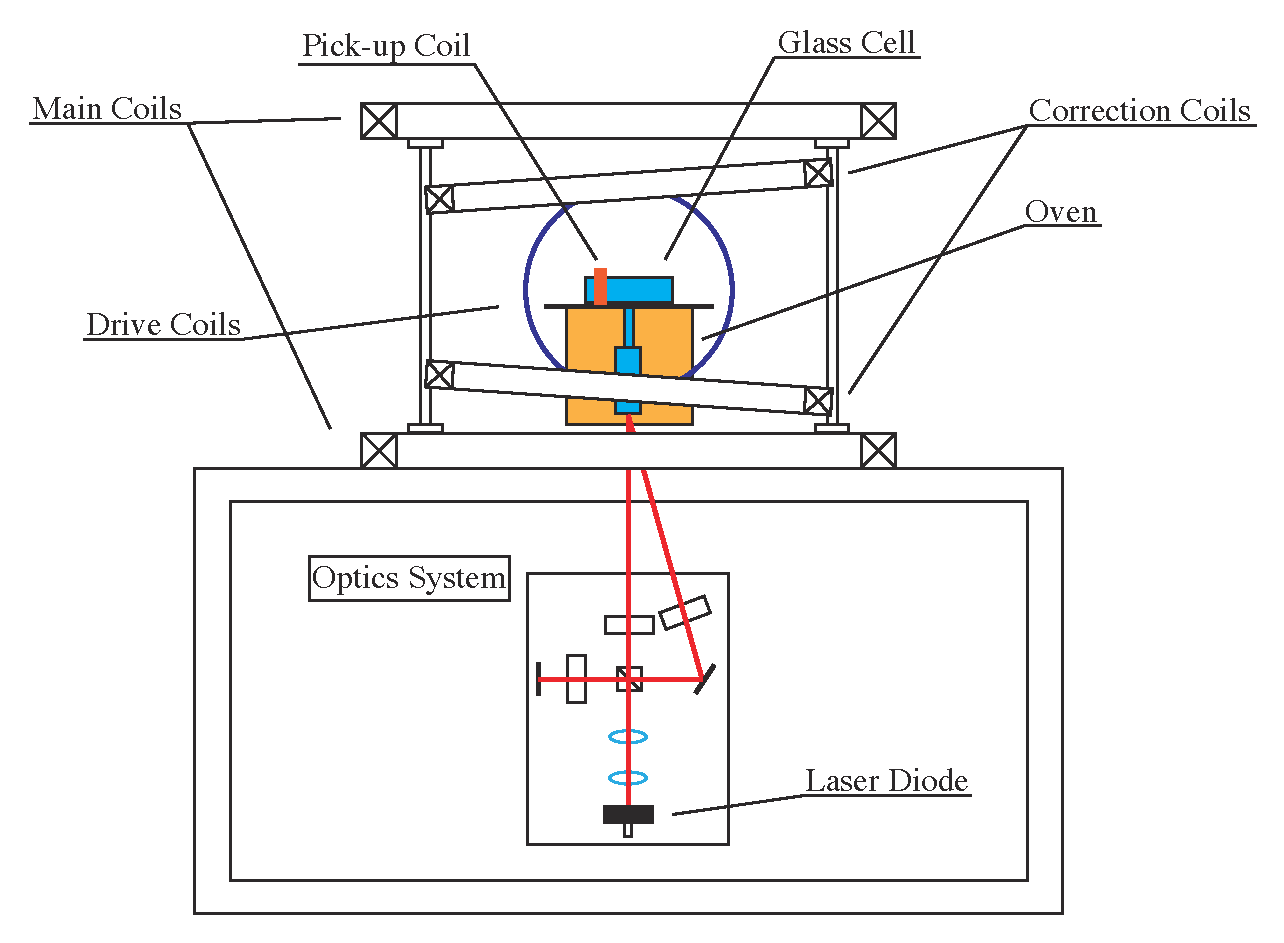
\includegraphics[clip,width=11cm]{./chap3/fig/pol-sys_sche.pdf}\\
%  \caption{偏極$^3$He標的の概略図}
%  \label{pol-sys}
% \end{figure}

% %%%% 3.1 %%%%
%  \section{${}^3$He標的セル}
%  \label{sec:tar_cell}
% 我々は、陽子--$^3$He弾性散乱実験に用いる標的として、$^3$Heガスをガラスセルに封入した標的セルを製作した。ガラスセルの素材としてはGeneral Electric社のアルミノ珪酸ガラスであるGE180を用いた。GE180は、ガラス中に含まれる磁性不純物の量が少ないため、不純物との相互作用による$^3$Heの核スピンの偏極緩和率が小さいことが知られている\cite{Jia13}。またCorning社のpyrexガラス等に比べ、$^3$Heガスの透過率が低く、長期間高密度の状態を維持することが可能である。\\
%  我々のグループが製作した標的セルの典型的な形状を図\ref{kuki}に示す。標的セルは、散乱実験でビームを照射する標的部とRb蒸気を発生させるためにオーブンに入れるポンピング部から成るダブルセル構造である。$^3$He原子核は、ポンピング部でRbとのスピン交換によって偏極し、その後拡散することで標的部へと移動する。この時Rb蒸気も標的部に移動しないように、標的部およびポンピング部を繋ぐ管は$\phi10~{\rm mm}$の外径かつ$65~{\rm mm}$の長さにしてある。また$3$気圧の高密度の$^3$Heガスを想定し、ガラスセルの厚さは約$1~{\rm mm}$とした。標的部のビーム入射面および出射面は、入射ビームのエネルギー損失を出来るだけ小さくするために約$0.5~{\rm mm}$の厚さとし、また強度を高めるために半球形に凹ませている。

% \begin{figure}[tbp]
%  \centering
%  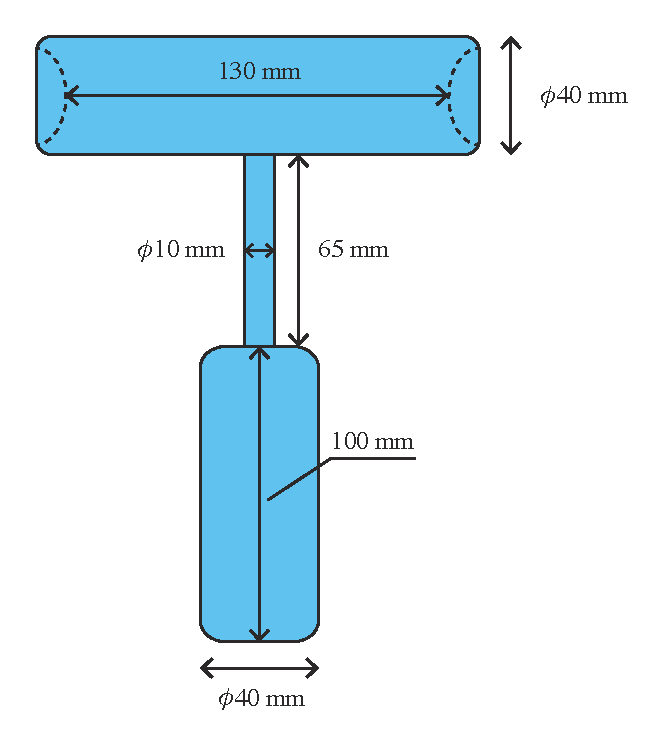
\includegraphics[clip,width=6cm]{./chap3/fig/kuki_sche.pdf}\\
%  \caption{製作したセルの典型的な形状}
%  \label{kuki}
% \end{figure}

% 以下の節では、この標的セルの製作装置および製作方法について述べる。

% %% 3.1.1 %%
%   \subsection{標的セルの製作装置}
% SEOP法によって$^3$He原子核を偏極させるためには、$^3$Heガスの他にRbおよびN$_2$ガスをガラスセルに封入する必要がある。また2.3.2節でも述べたように、$^3$He原子核の偏極度を高めるためには$^3$He原子核の偏極緩和率を小さくすることが重要である。従って、ガラスセルの洗浄や真空引き、ベーキング等によってセル内部の不純物を取り除くことが必要である。\\
%  標的セルの製作装置の模式図を図\ref{vac-sys}に示す。セル製作装置は、ガラスセルが繋がれているセルブランチ、真空引きを行うためのロータリーポンプおよびターボ分子ポンプ(TMP)、真空度を測定するためのバラトロンゲージやクリスタルゲージおよびペニングゲージ、そして$^3$HeガスやN$_2$ガスを純化して導入するためのゲッターから構成される。

% \begin{figure}[tbp]
%  \centering
%  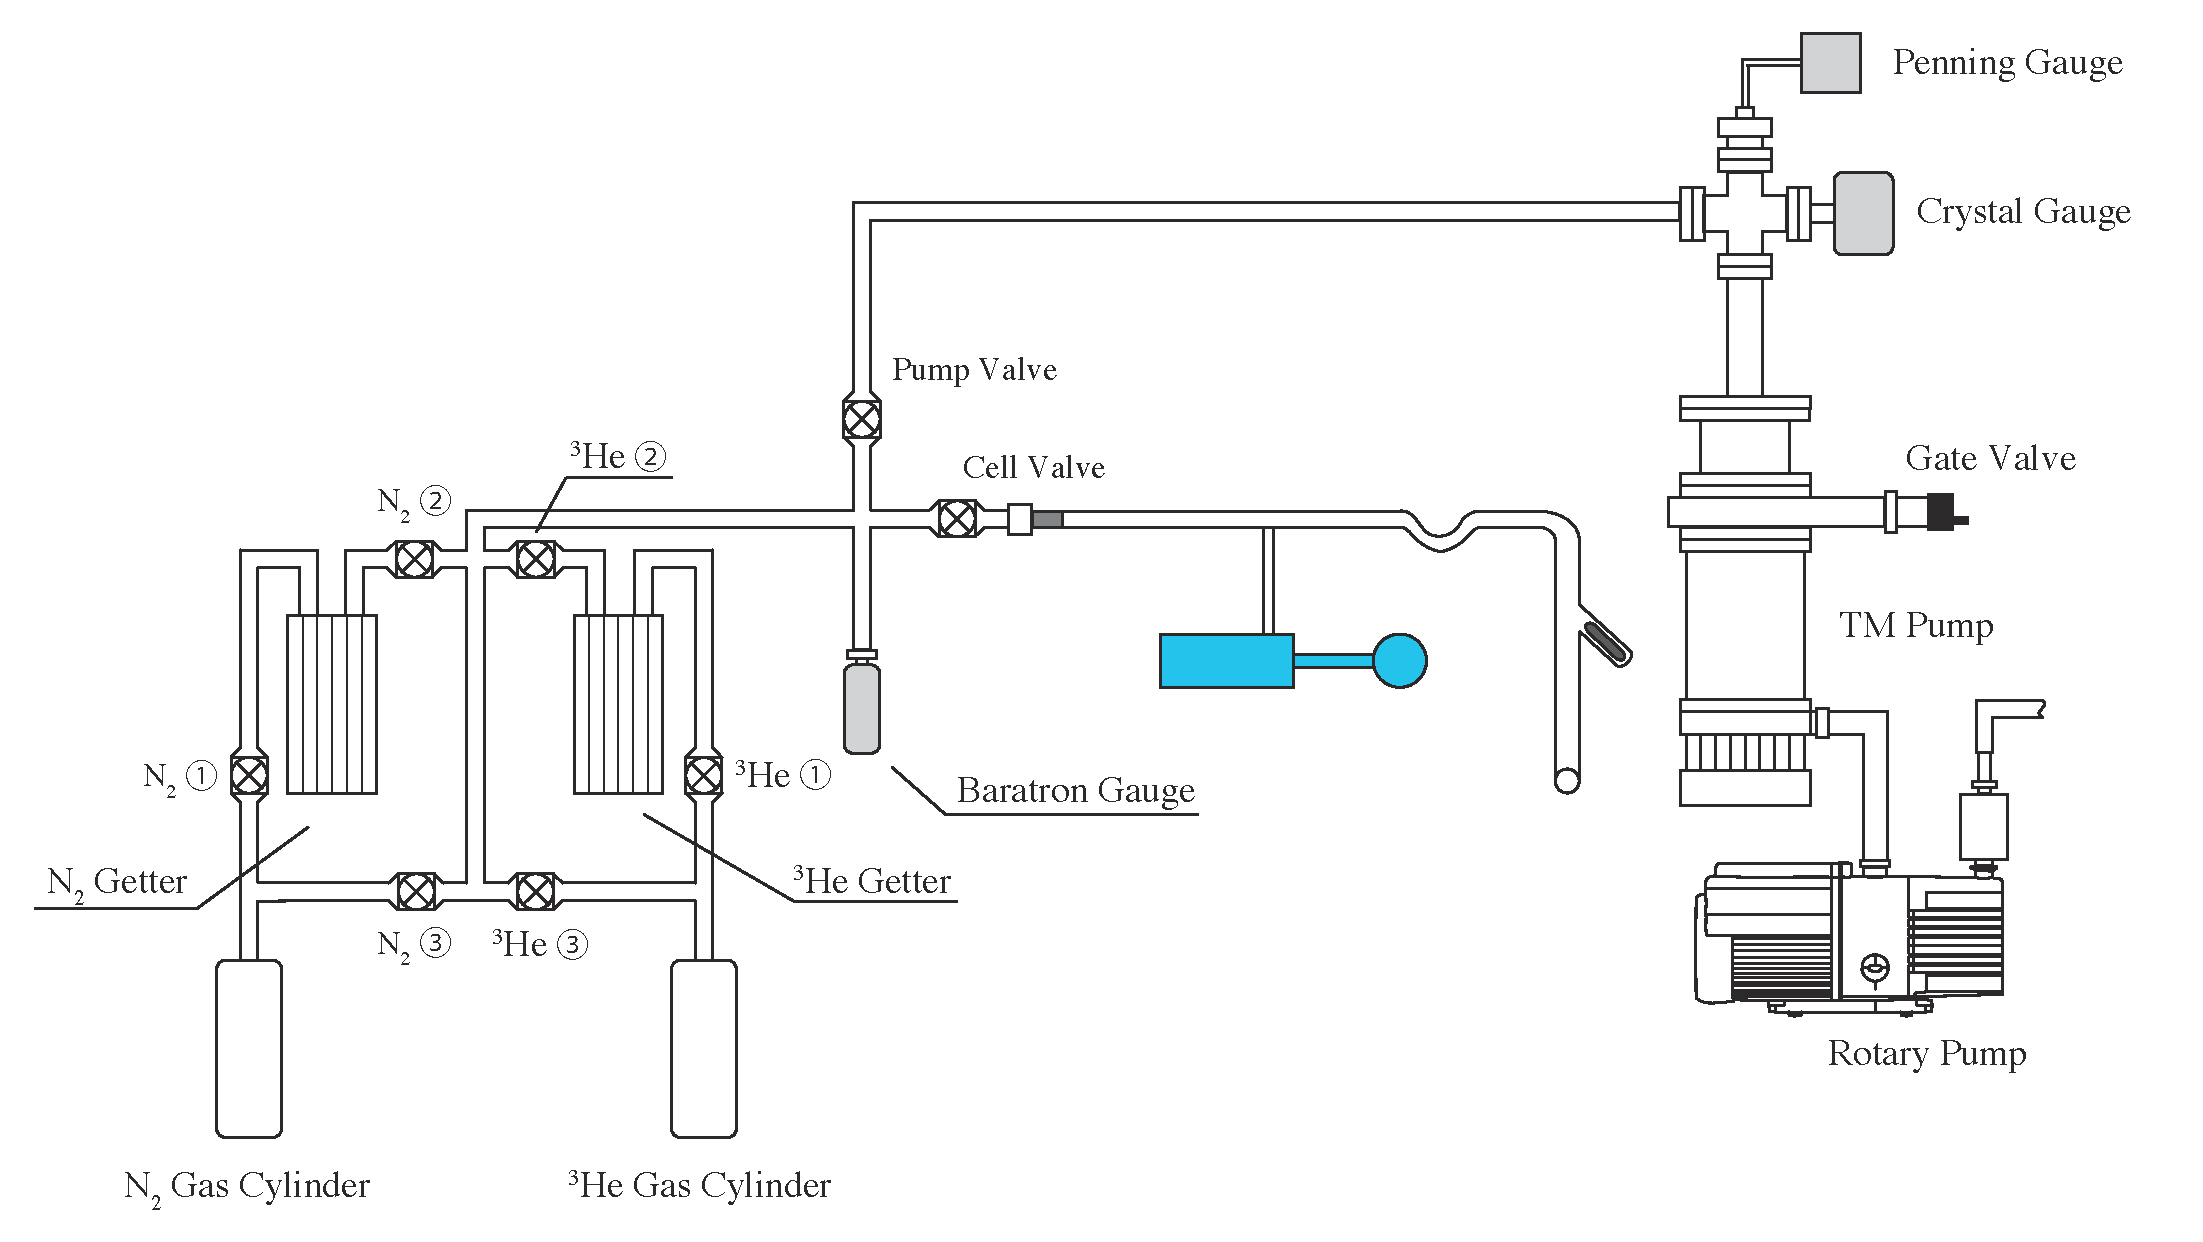
\includegraphics[clip, width=1.0\linewidth]{./chap3/fig/vacuum-sys.pdf}\\
%  \caption{標的セル製作装置の模式図}
%  \label{vac-sys}
% \end{figure}

% \begin{figure}[tbp]
%  \centering
%  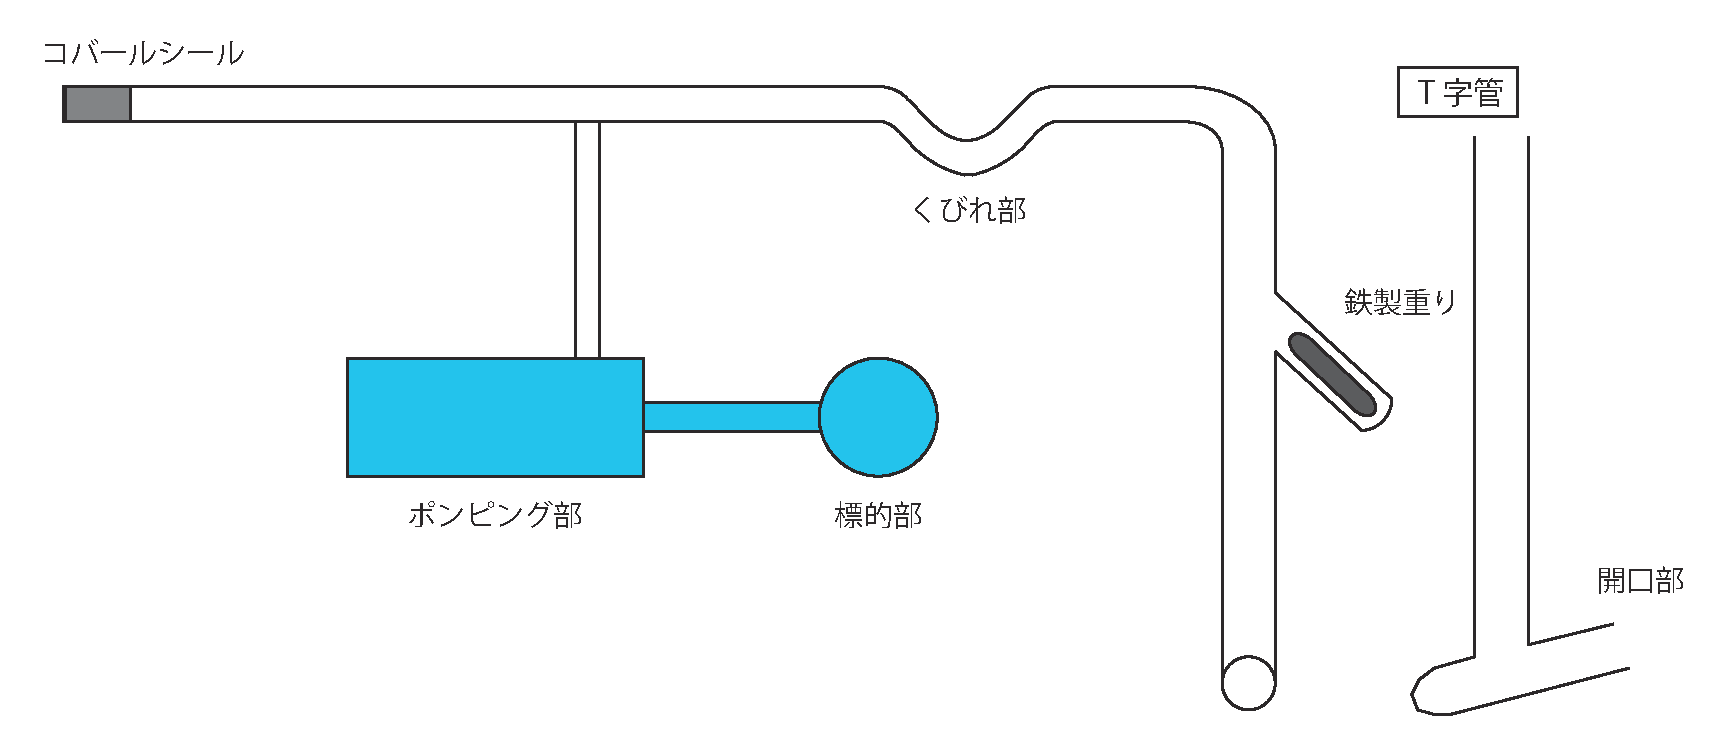
\includegraphics[clip, width=1.0\linewidth]{./chap3/fig/cell-branch.pdf}\\
%  \caption{セルブランチの概略図。水色の領域は標的セルの部分。}
%  \label{cell-bra}
% \end{figure}

% セルブランチの概略図を図\ref{cell-bra}に示す。標的セルは初めセルブランチに繋がれており、端にコバールシールを溶接して真空排気系と接続している。標的セルの素材であるGE180はバーナー等による加工が難しいため、標的セル以外の部分は比較的加工が容易であるpyrexガラスを使用した。標的セルとセルブランチとは$\phi8~{\rm mm}$のガラス管で接続されており、このガラス管を通して真空引きや洗浄液の流入による標的セル内の洗浄を行う。またセルブランチの“T字管”部分には、純度$99.9%$のRb $1~{\rm g}$が入ったアンプル(93-3736, STREM社)を導入するための開口部がある。開口部からRbアンプルを入れてバーナーで封じ切った後、鉄芯を磁石で持ち上げて落とすことでアンプルを割る。鉄芯は、セル内の高真空度を保つためにpyrexガラスで包まれている。\\
%  セルブランチの真空引きは、ロータリーポンプ(RV-12, EDWARDS社)およびターボ分子ポンプ(TMP280, 島津製作所)によって行う。これらの真空排気系による典型的な到達真空度は$4.5 \times 10^{-5}~{\rm Pa}$である。\\
%  真空度はクリスタルゲージ(M-320XG, キャノンアネルバ社)およびペニングゲージ(TPG300, BALZERS社)によって測定した。クリスタルゲージは水晶振動子の共振インピーダンスが圧力に応じて変化する性質を利用した真空計で、$10^5〜10^{-2}~{\rm Pa}$の範囲の圧力を測定できる。またペニングゲージは真空中に残留する気体を電離させ、それによって生成されるイオンや電子を電極で捕集することで流れる電流から圧力を測定する真空計である。クリスタルゲージよりも高い真空度を測定でき、およそ$10^{-9}~{\rm Pa}$の低圧力まで測定が可能である。\\
%  $^3$HeガスおよびN$_2$ガスを標的するに封入する時の圧力は、バラトロンゲージ(750B, mks社)によって測定した。バラトロンゲージは差圧によって薄い金属膜を変形させ、それに応じて変化する静電容量の値から圧力を測定する真空計であり、大気圧のおよそ$10^{-2}$倍から$10^2$倍までの範囲の圧力を測定できる。またバラトロンゲージは、圧力に対応した電圧値を出力するので、圧力の較正を行う必要がある。図\ref{bara_calib_fig}に、バラトロンゲージの較正結果を示す。横軸はアネロイド気圧計(7610-20, 佐藤計量器製作所)で測定した圧力、縦軸はバラトロンゲージの出力電圧値を示している。一次関数でフィッティングした結果、圧力$Prs$に対するバラトロンゲージの出力電圧値$V_{\rm bara}$の関係は
% %
% \begin{equation}
%  V_{\rm bara}~[{\rm V}] = (1.513 \pm 0.003) \times 10^{-3} Prs~[{\rm hPa}] - (0.5 \pm 1.0) \times 10^{-3}
%  \label{bara_calib}
% \end{equation}
% %
% となった。

% \begin{figure}[tbp]
%  \centering
%  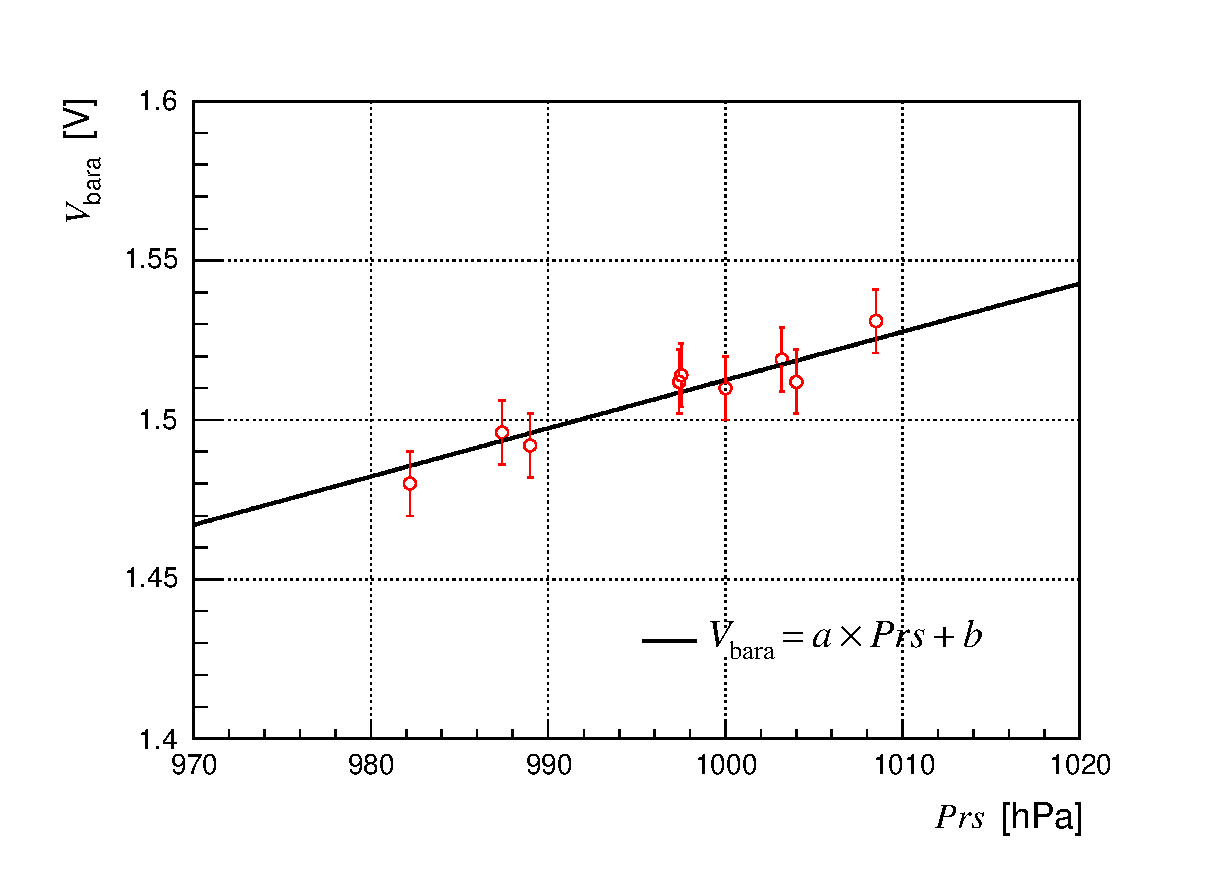
\includegraphics[clip, width=10cm]{./chap3/fig/Bara_calib.eps}\\
%  \caption{バラトロンゲージの較正結果}
%  \label{bara_calib_fig}
% \end{figure}

% 標的セルに$^3$HeガスおよびN$_2$ガスを封入する際は、ゲッターを通して不純物を除去し、純化させる。ゲッターはsaes gettes社のGC50(He用:PS2-GC50-R-1, N$_2$用:PS2-GC50-N-1)を用いた。これによって、$^3$Heガスは$99.999%$、N$_2$ガスは$99.999999%$までの純度にすることが可能である。

% %%%%%%%

% %% 3.1.2 %%
%   \subsection{標的セルの製作方法}
% 上記のセル製作装置を用いて、標的セルの製作を行った。セル製作の手順を以下に示す。
% %
% \begin{itemize}
%  \item ガラスセルの洗浄
%  \item Rbアンプル導入
%  \item ベーキングおよびRbアンプル割り
%  \item Rbの移送
%  \item $^3$HeガスおよびN$_2$ガス封入
% \end{itemize}
% %
% 以下では、これらの項目それぞれについて述べる。
% %
% \begin{description}
%  \item[ガラスセルの洗浄]  
%  %
%  \begin{enumerate}
%   \item セル内の金属化合物や油脂等を取り除くために、$10%$程度に希釈した中性洗剤を用いて洗浄する。 希釈した洗剤溶液を$50℃$程度まで温め、セルブランチを約6時間浸す。この時、1時間毎にセルブランチ内の洗剤溶液の入れ替えを行う。
%   \item 純水で5回以上すすぎ、洗剤溶液を洗い流す。
%   \item アセトンで3回以上すすぎを行う。
%   \item エタノールで3回以上すすぎを行う。
%  \end{enumerate}
%  %
% \end{description}
% %
% \begin{description}
%  \item[Rbアンプル導入]  
%  %
%  \begin{enumerate}
%   \item セルブランチの洗浄後、真空排気系に接続する。この時、ガスラインにN$_2$ガスを充填させておく。これによって、接続時に不純物が真空排気系に流入するのを防ぐ。
%   \item N$_2$ボンベを開け、セルブランチのT字管の開口部からN$_2$ガスが流れ出るようにする。
%   \item ヒートガンでT字管を加熱し、エタノールを蒸発させる。
%   \item Rbアンプルを開口部から投入し、N$_2$ボンベを閉じて開口部をバーナーで封じ切る。
%   \item セルバルブおよびポンプバルブを開け、真空引きを開始する。
%   \item 再びヒートガンで加熱して、セルブランチ内のエタノールを蒸発させ取り除く。
%   \item 10時間程度真空引きを行う。
%  \end{enumerate}
%  %
% \end{description}
% %
% \begin{description}
%  \item[ベーキングおよびRbアンプル割り]  
%  %
%  \begin{enumerate}
%   \item Rbアンプル以外の部分にリボンヒーターを巻き、約$235℃$まで加熱しベーキングを行う。
%   \item 3日間程度ベーキングを行う。
%   \item ベーキングを停止し、ポンプバルブを閉じる。
%   \item セルブランチに$1$気圧程度N$_2$ガスを充填する。
%   \item 磁石で鉄芯を持ち上げ落とし、Rbアンプルを割る。
%   \item アンプル内の不活性ガスを取り除くために、ポンプバルブを開けて再びベーキングおよび真空引きを行う。
%   \item 真空度が$\sim 10^{-5}~{\rm Pa}$程度になるまでベーキングおよび真空引きを続ける。
%  \end{enumerate}
%  %
% \end{description}
% %
% \begin{description}
%  \item[Rbの移送]  
%  %
%  \begin{enumerate}
%   \item ベーキングを停止し、セルブランチが常温程度まで冷えるのを待つ。
%   \item くびれ部を送風で冷やしながら、T字管にリボンヒーターを巻いて加熱し、Rbをくびれ部に移送する。
%   \item くびれ部に十分な量のRbが溜まったら、ポンプバルブを閉じる。
%   \item セルブランチ内に$1$気圧程度N$_2$ガスを充填し、T字管をバーナーで切り落とす。
%   \item ポンプバルブを開け、くびれ部以外の部分にリボンヒーターを巻き、ベーキングおよび真空引きを行う。
%   \item 真空度が$\sim 10^{-5}~{\rm Pa}$程度になるまでベーキングおよび真空引きを続ける。
%   \item ヒートガンで加熱し、標的セル内にRbを移送する。
%   \item 10時間程度真空引きを行う。
%  \end{enumerate}
%  %
% \end{description}
% %
%  \begin{description}
%  \item[$^3$HeガスおよびN$_2$ガス封入]  
%  %
%  \begin{enumerate}
%   \item ポンプバルブを閉じ、真空引きを停止する。
%   \item 標的セルを液体窒素に浸し、標的セル内部の温度を窒素の沸点($=-195.8℃$)まで冷却する。
%   \item N$_2$ボンベを開け、セルブランチ内にガスを送る。この時、GC50を通過させてガスを純化する。
%   \item バラトロンゲージの圧力を読みながら、常温でN$_2$ガスの圧力が約$100~{\rm Torr}$となるように調整する。
%   \item セルバルブを閉じ、ポンプバルブを開けて真空排気系の真空引きを行う。
%   \item ポンプバルブを閉じ、$^3$Heボンベを開けてセルブランチ内にガスを導入する。この時、N$_2$ガス同様GC50を通過させてガスを純化する。
%   \item バラトロンゲージの圧力を読みながら、$^3$Heガス圧力が$1$気圧程度になるよう調整する。これによって、常温で$^3$Heガス圧力が約$3$気圧となる。
%   \item バーナーで標的セルとセルブランチを繋いでいるガラス管を封じ切る。
%  \end{enumerate}
%  %
% \end{description}
% %
% 以上の過程により、陽子--$^3$He弾性散乱実験で使用する標的セル“Kuki”を製作した。
 
% %%%%%%%
% %%%%%%%%%%

% %%%% 3.2 %%%%
%  \section{偏極生成装置}
% $^3$He原子核の偏極生成装置は、静磁場を発生させるためのメインコイルおよび補正コイル、Rb蒸気を発生させるためにガラスセルを加熱する標的オーブン、Rbの光ポンピングのための半導体レーザーおよび光学系から構成される。本節では、これらの装置それぞれについて述べる。

% %% 3.2.1 %%
%   \subsection{静磁場発生用コイル}
% スピンの量子化軸を決めるための静磁場は、メインコイルおよび補正コイルの二組のコイルによって発生させている。メインコイルは、標的セル周辺の領域での静磁場の均一度を高めるために、ヘルムホルツ型のコイルを採用している。補正コイルは図\ref{pol-sys}のようにヘルムホルツコイルを上下に少し傾けたものであり、メインコイルによって作られる静磁場の均一度を調整するために用いられる。メインコイルおよび補正コイルの仕様を表\ref{coils}に示す。メインコイルは、数 Aの電流で$1〜3~{\rm mT}$の静磁場を発生させることができる。この時発生させる静磁場の向きは鉛直下向きである。また発生させる静磁場の均一度は、ヘルムホルツコイルの中心から標的セルの長さである$15~{\rm cm}$の領域において$10^{-3}~{\rm cm^{-1}}$程度である。
% %
%  \begin{table}[htbp]
%   \caption{メインコイルおよび補正コイルの仕様}
%   \centering
%   \begin{tabular}{|c||c|c|} \hline
% & メインコイル & 補正コイル \\ \hline
% 直径 & $100~{\rm cm}$ & $75~{\rm cm}$ \\
% 導線の太さ & $\phi 1.7~{\rm mm}$ & $\phi 1.7~{\rm mm}$ \\
% 巻き数 & 300 回 & 100 回 \\ \hline
%   \end{tabular}
%   \label{coils}
%  \end{table}\\
% %
%  メインコイルに流れる電流$I_{\rm main}$と中心部におけるメインコイルが作る静磁場の$z$成分$B_z$の関係を図\ref{main-coil}に示す。図\ref{main-coil}のグラフは、最小二乗法によって一次関数でフィッティングした結果を示している。フィッティングの結果、$I_{\rm main}$と$B_z$の関係式は
% %
% \begin{equation}
%  B_z~[{\rm mT}] = (0.498 \pm 0.016) \times I_{\rm main}~[{\rm A}] - (0.091 \pm 0.062)
%  \label{Bz-Imain}
% \end{equation}
% %
% となった。およそ$6~{\rm A}$の電流を流すことによって、$3~{\rm mT}$程度の静磁場を発生させることができる。メインコイルおよび補正コイルの電源は工藤電機製の直流電源(作番 030058)を用いた。この直流電源はTTL規格のトリガー信号を入力することで、設定された二つの電流値の間を掃引させることができる。

% \begin{figure}[tbp]
%  \centering
%  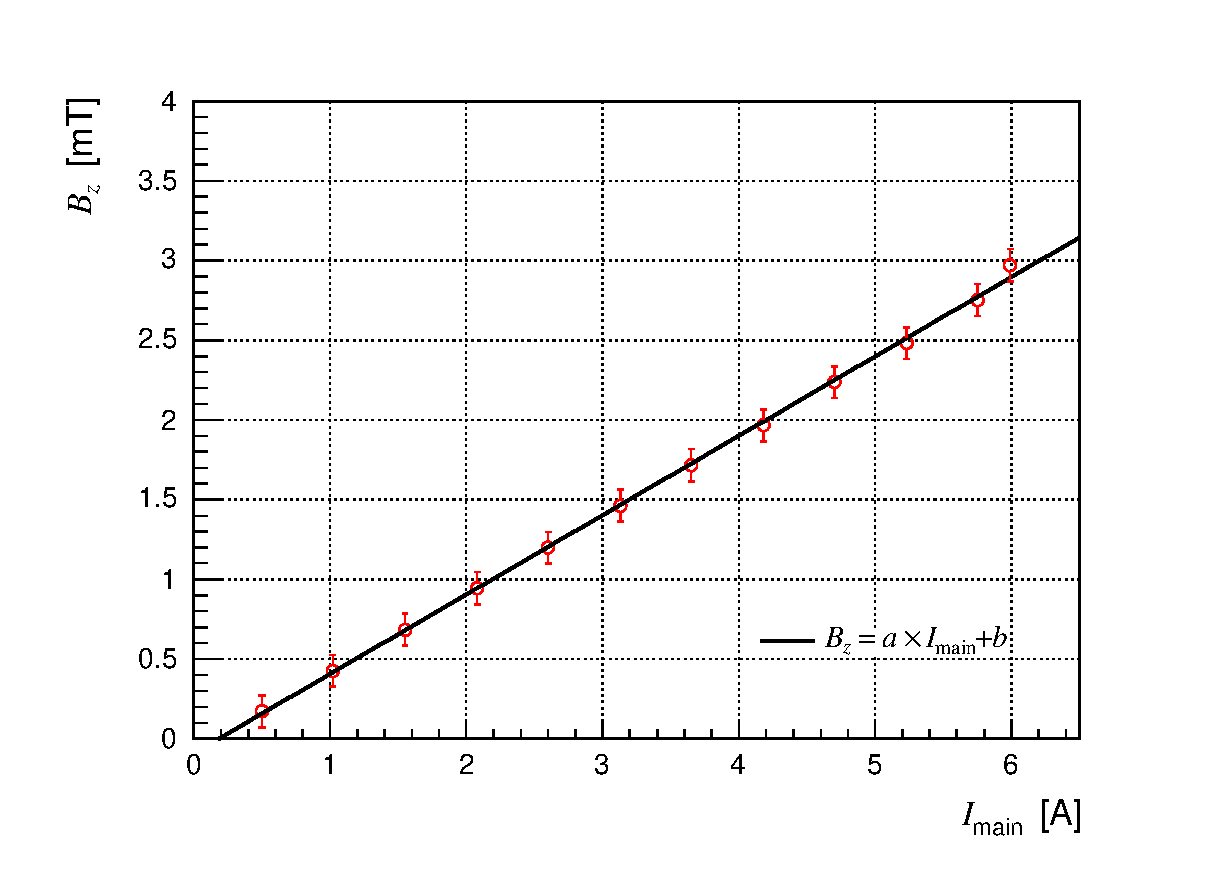
\includegraphics[clip, width=10cm]{./chap3/fig/Main_Coil.eps}\\
%  \caption{メインコイルの励磁曲線}
%  \label{main-coil}
% \end{figure}

% %%%%%%%

% %% 3.2.2 %%
%   \subsection{標的オーブン}
% 標的セル内のポンピング部に光ポンピングするにあたって十分な量のRb蒸気を発生させるためには、ポンピング部を$200$℃程度の高温にまで加熱する必要がある。そこで、標的セルのポンピング部のみを標的オーブン内に入れ、熱風によって加熱させる方法を取った。標的オーブンの材質は、非磁性かつ高い耐熱性を持つポリエーテルエーテルケトン(PEEK)を採用した。標的オーブンの模式図を図\ref{oven}に示す。オーブンのビーム軸方向の側面および底面はガラス窓が取り付けられており、下方向からガラス窓を通してレーザーを照射する。オーブン内は、ポンピング部の側面にアルミ製のダクトを通して熱風機(Hot-Wind System, LEISTER社)から熱風を送ることで高温に保つ。また熱風機の出す熱風の温度および風量は外部信号入力による制御が可能であり、ファンクションジェネレーター(FG120, YOKOGAWA社)からの出力を外部入力信号として用いた。ファンクションジェネレーターはLinuxコンピューターによるGPIB制御で動作させており、これによって標的オーブン内の温度を一定に保つようにした。標的オーブン内の温度は白金測温抵抗体(Pt100)を用いて測定した。

% \begin{figure}[tbp]
%  \centering
%  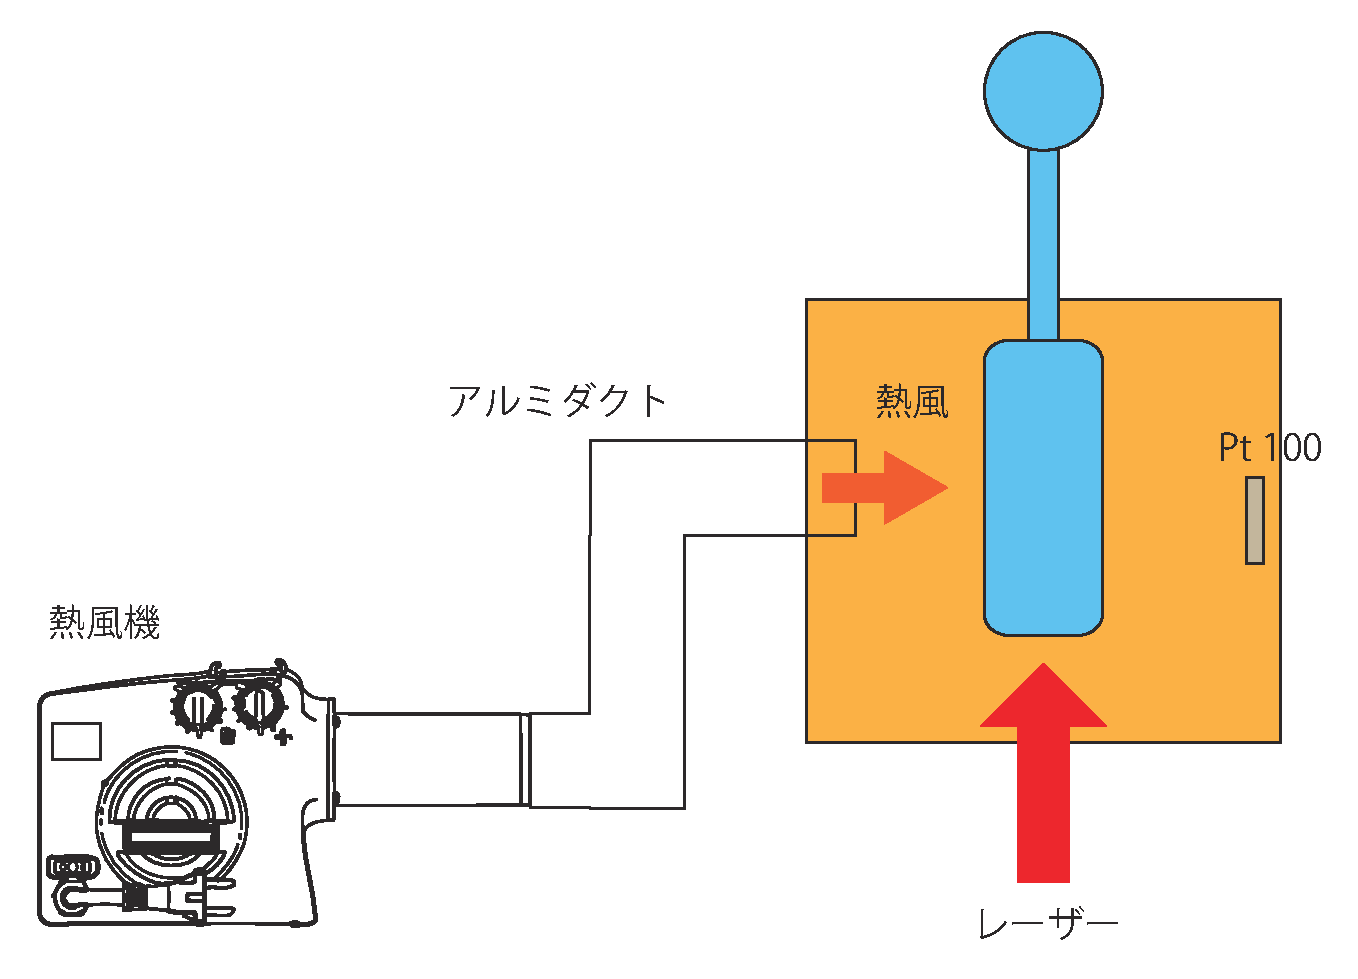
\includegraphics[clip, width=8cm]{./chap3/fig/oven_sche.pdf}\\
%  \caption{標的オーブンの模式図}
%  \label{oven}
% \end{figure}

% %%%%%%%

% %% 3.2.3 %%
%   \subsection{半導体レーザー}
% 光ポンピングによってRb原子を偏極させるためのレーザーとして、ファイバー結合型高出力半導体レーザー(FAP-79-30C-800-B, COHERENT社)を用いた。半導体レーザー本体は二つのレーザーアレイパッケージで構成されており、それぞれのレーザーアレイには光ファイバーが結合されている。またこれらの二つのファイバーはひとつにまとめられ、単一のファイバー端子として使用することができる。本研究で使用した半導体レーザーの仕様を表\ref{LD}に示す。半導体レーザーの電源はLumina Power社のLDD-250-4-6を用い、二つのレーザーアレイに対し直列に繋いだ。
% %
%  \begin{table}[htbp]
%   \caption{半導体レーザーの仕様}
%   \centering
%   \begin{tabular}{|c|c|} \hline
% 中心波長 & $795~{\rm nm}$ \\
% FWHM & ${< 4~\rm nm}$ \\
% 最大出力& $30~{\rm W}$ \\
% ファイバーコア径 & $800~{\rm \mu m}$ \\
% 開口数 & $< 0.16$ \\ \hline
%   \end{tabular}
%   \label{LD}
%  \end{table}\\
% %
%  本研究で使用した半導体レーザーの励起曲線を図\ref{laser-pow}に示す。図\ref{laser-pow}において、横軸はレーザー電源の出力電流、縦軸はパワーメーター(PM150-50, Molectron社)で測定したレーザー出力である。レーザーは電源の供給電流$8~{\rm A}$程度から発振し始め、その後は供給電流に対して線形に出力が増加していく。供給電流に対するレーザー出力の比はおよそ$1.14~{\rm W/A}$である。

% \begin{figure}[tbp]
%  \centering
%  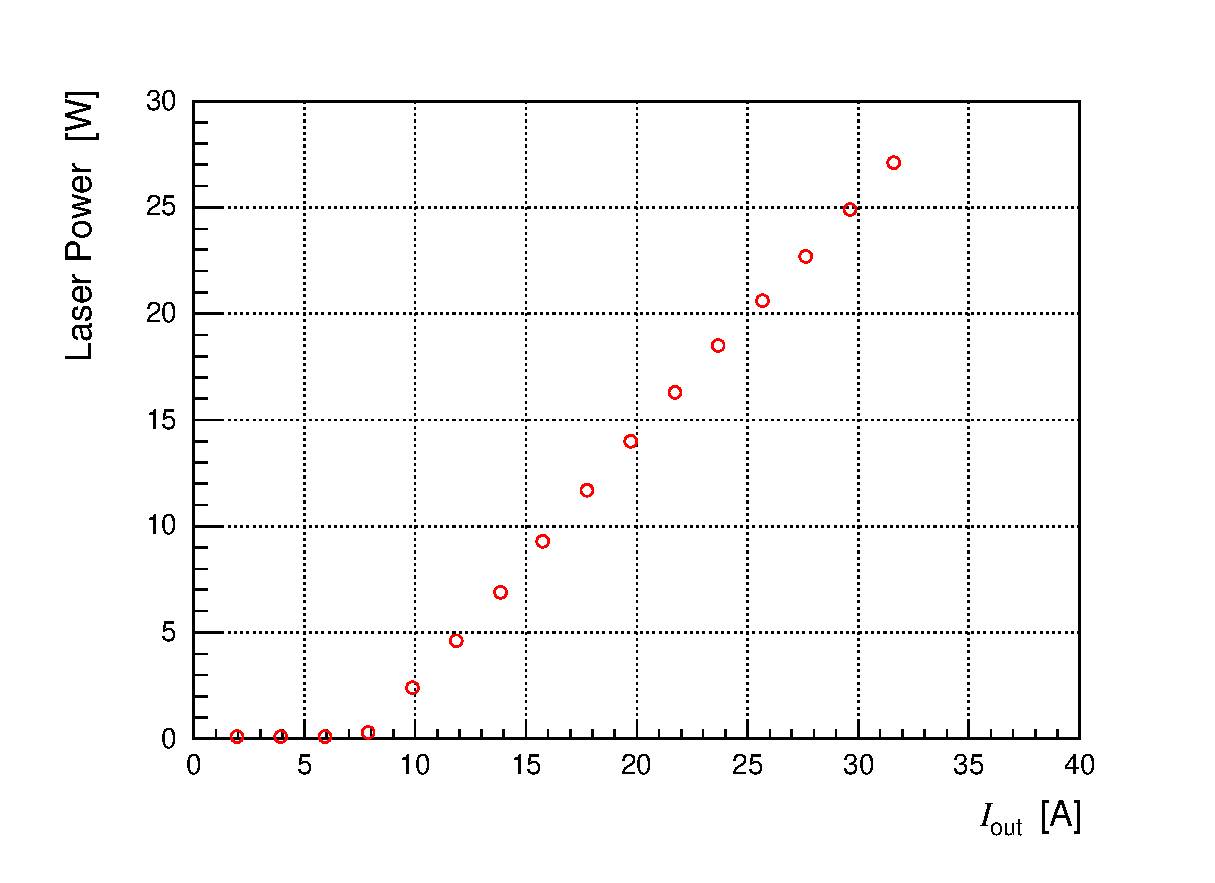
\includegraphics[clip, width=10cm]{./chap3/fig/Laser_Pow-Iout.eps}\\
%  \caption{半導体レーザーの励起曲線}
%  \label{laser-pow}
% \end{figure}

% 半導体のバンドギャップおよび光共振器として用いる半導体結晶の劈開面の距離は温度に依存する。よって、レーザー素子の温度を調整することで発振するレーザー波長を変化させることができる。そこでレーザー本体の温度を制御するために、レーザー本体を排気扇付きの空冷箱に固定し、銅板を介してPeltier素子を取り付けた。Peltier素子は、二種類の金属の接合部に電流を流すと、一方の金属からもう一方の金属へと熱が伝導していくPeltier効果を利用した半導体素子で、流す電流値を調整することでレーザー本体の温度を調整できる。レーザー本体の温度は、温度センサー(LM335)をレーザー本体に取り付け測定した。またPeltier素子に電流を流す直流電源(E3642A, Agilent社)をGPIB制御で動作させることにより、レーザー本体の温度を調整および安定させた。\\
%  レーザーの中心波長が$795~{\rm nm}$になるレーザー温度を確認するために、定期的にレーザー波長の温度依存性測定を行った。典型的なレーザー温度に対するレーザー波長の測定結果を図\ref{laser_wl}に示す。レーザーの波長はADVANTEST社のデジタル光波長計(TQ8325)を用いて測定した。測定結果から、レーザー温度を$31$℃にすることで波長が$795~{\rm nm}$となることが分かる。

% \begin{figure}[tbp]
%  \centering
%  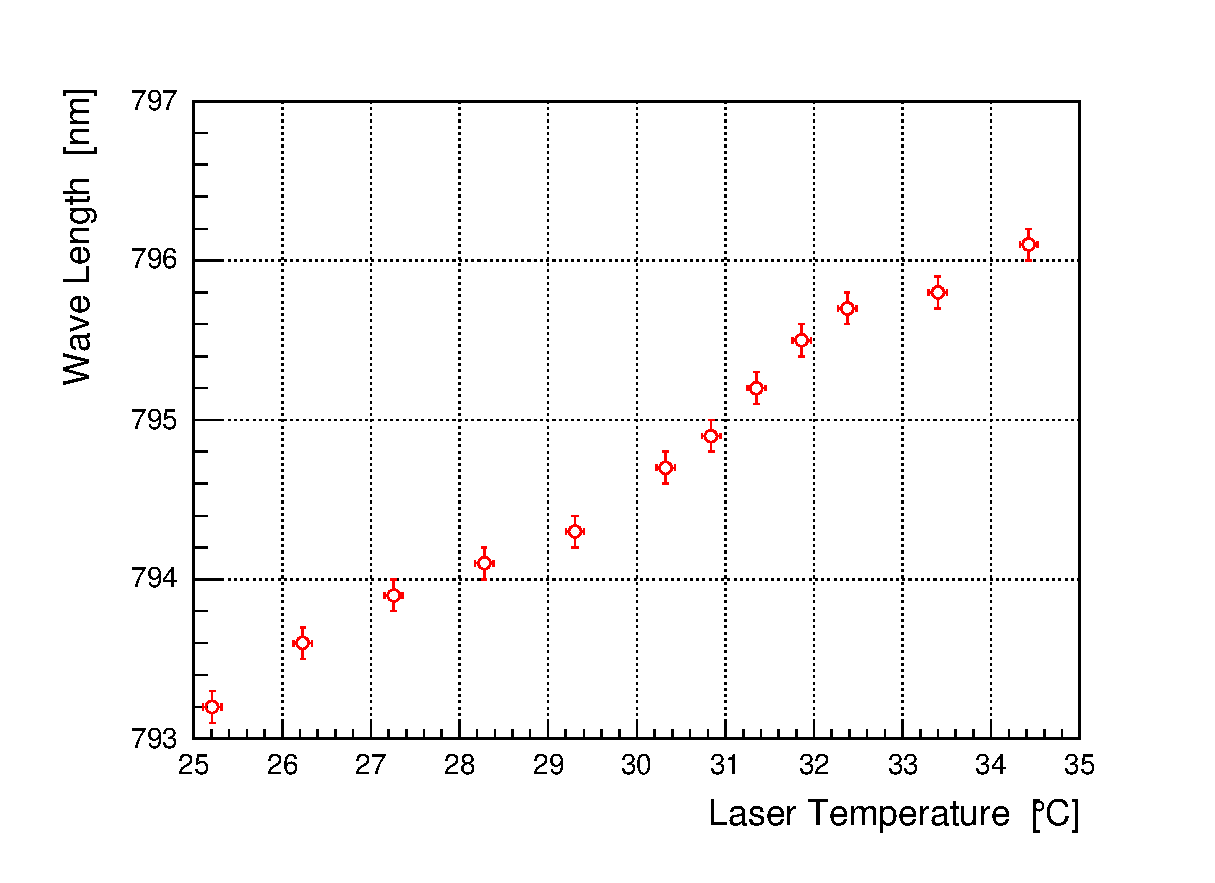
\includegraphics[clip, width=10cm]{./chap3/fig/Laser_wl.eps}\\
%  \caption{半導体レーザーの波長の温度依存性}
%  \label{laser_wl}
% \end{figure}

% %%%%%%%

% %% 3.2.4 %%
%  \subsection{光学系}
% 光ポンピングによってRb原子を偏極させるためには、円偏光レーザーを照射する必要がある。しかし、光ファイバーからのレーザー光は偏光を保存せず、非偏光状態である。そこで、偏光ビームスプリッター(PBS)や1/4波長板($\lambda/4$板)を用いて円偏光を生成するための光学系を組んだ。本研究で用いた光学系の模式図を図\ref{laser-sys}に示す。PBSは二つの直角プリズムにより構成される光学素子で、接合面にコーティングされた誘電体多層膜により入射した光をその偏光方向によって反射もしくは透過させる。そのため、図\ref{laser-sys}においてレーザーファイバーから照射された光は、PBSによって透過光であるP偏光(偏光方向が紙面に対して平行)の光と、反射光であるS偏光(偏光方向が紙面に対して垂直)の光に分けられる。透過光および反射光は1/4波長板を透過して標的セルへと照射される。1/4波長板は異方性媒質の結晶によって構成される光学素子で、直交する進相軸および遅相軸を透過した直線偏光の間で$\pi/2$の位相差を生じさせる。よって、直線偏光を両軸に対して入射角度が$45^\circ$となるように入射させれば円偏光を生成することができる。

% \begin{figure}[tbp]
%  \centering
%  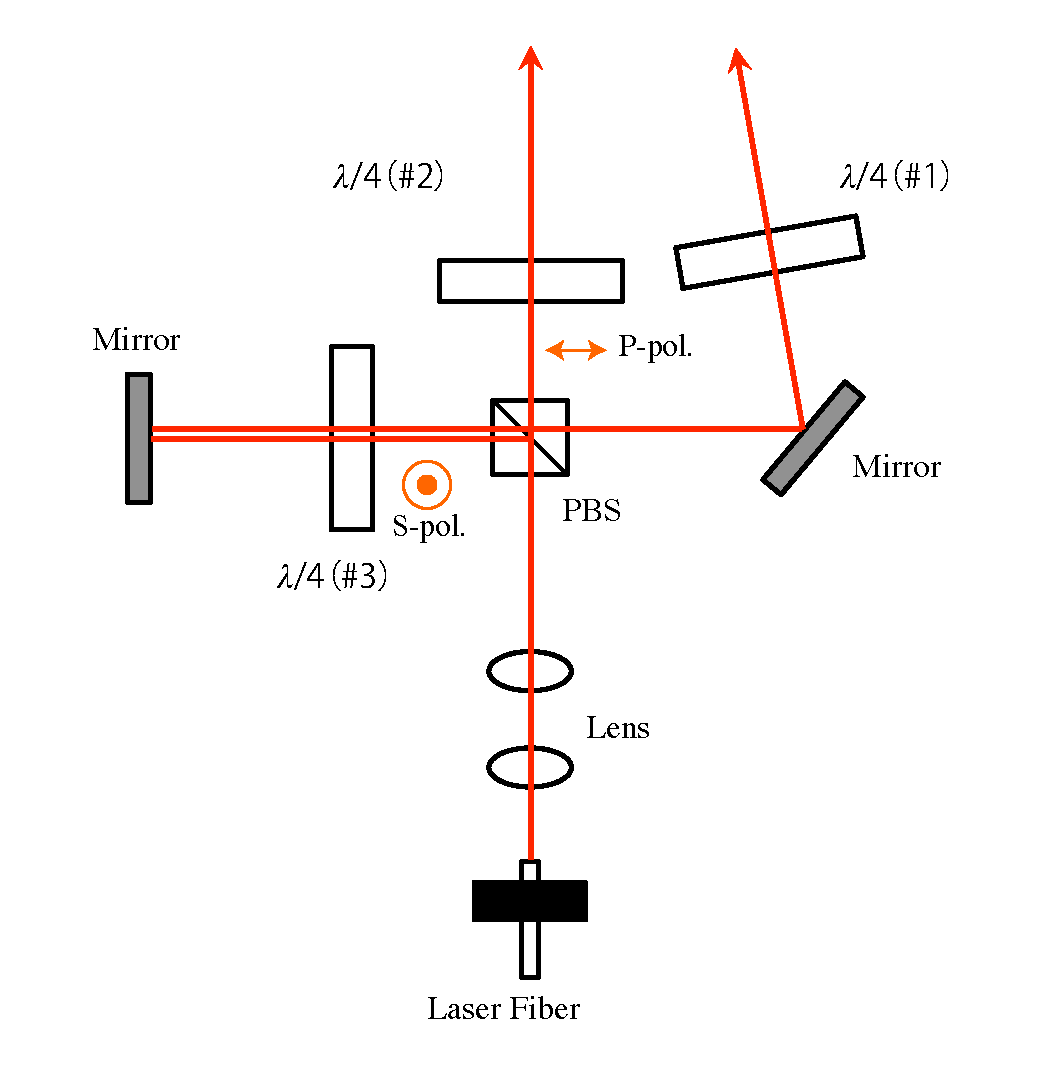
\includegraphics[clip, width=8cm]{./chap3/fig/laser-sys.pdf}\\
%  \caption{円偏光を生成するための光学系の模式図}
%  \label{laser-sys}
% \end{figure}

% PBSによって分離された直線偏光を1/4波長板を透過させて円偏光を生成する際、1/4波長板の角度の最適化が重要である。角度の調整は、図\ref{laser-sys}において1/4波長板の直後にPBSを置き、PBSを透過したレーザーの出力をパワーメーターで測定することで行う。PBSは前述のようにP偏光のみを透過させるため、1/4波長板通過前のレーザーがP偏光である場合は直線偏光となっている時に出力が最大、それに対して円偏光となっている時に出力が最小となる。また1/4波長板通過前のレーザーがS偏光である場合は直線偏光となっている時に出力が最小、円偏光となっている時に出力が最大となる。すなわち、1/4波長板の光軸周りの角度$\theta$に対応し、PBS透過後のレーザー出力は$1/2(1 \pm \cos^2 \theta)$に比例することになる。ここで、$+$はP偏光、$-$はS偏光を表す。\\
%  図\ref{laser-sys}において、\#2および\#3の1/4波長板通過後のレーザーに対して、PBS透過後のレーザー出力の測定結果を図\ref{lam4_2_3}に示す。この測定から、\#2および\#3の1/4波長板の角度を$49^\circ$および$139^\circ$にすることで円偏光が生成されることを確認した。また\#3の1/4波長板の角度を$139^\circ$に設定し、\#1の1/4波長板について同様の測定を行った。測定結果を図\ref{lam4_1}に示す。\#1の1/4波長板に関しても、同様に$49^\circ$および$139^\circ$にすることで円偏光の生成を確認した。よって、\#1、\#2および\#3の1/4波長板の角度は全て$49^\circ$または$139^\circ$に設定し、円偏光のレーザーによる光ポンピングを行う。

% \begin{figure}[tbp]
%  \centering
%  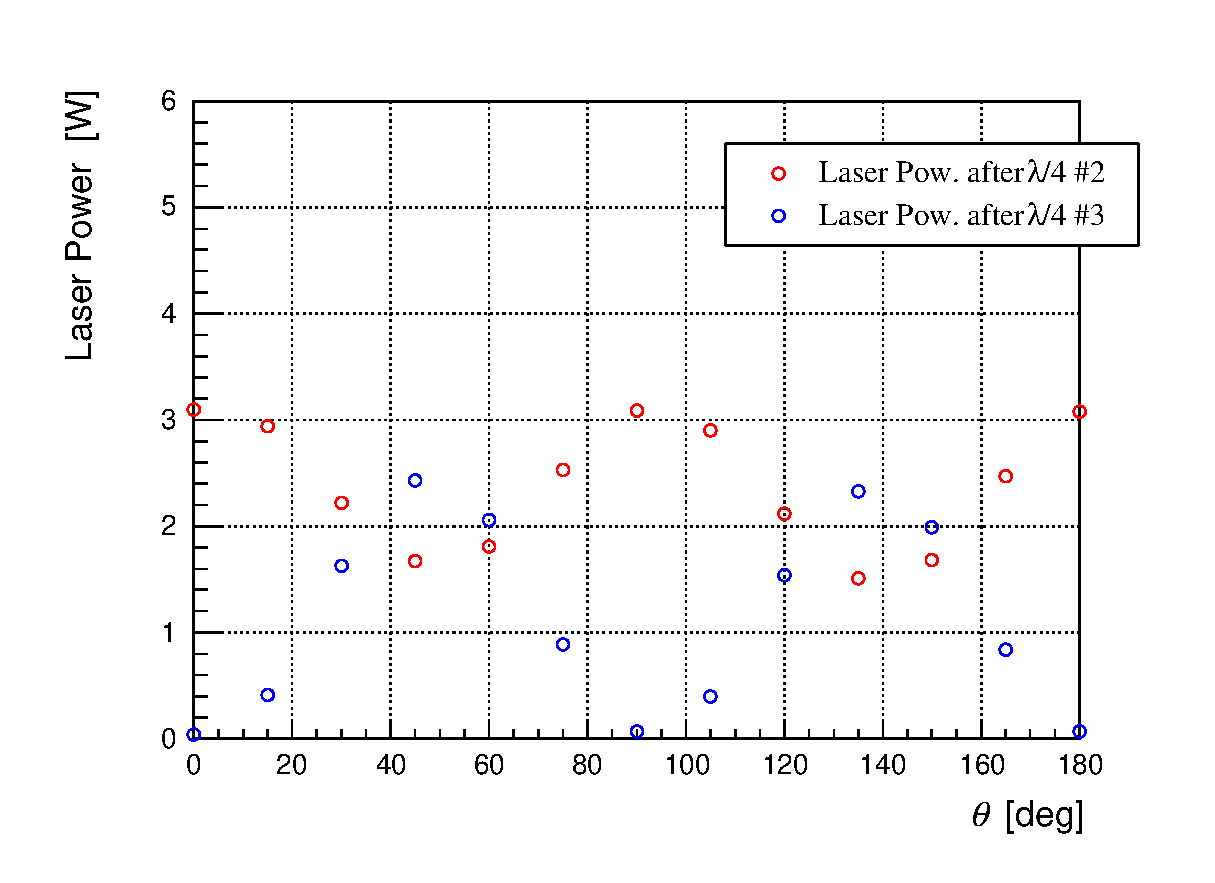
\includegraphics[clip, width=10cm]{./chap3/fig/lam4_2_3_Pow.eps}\\
%  \caption{1/4波長板の光軸周りの角度$\theta$に対するPBS透過光強度(\#2および\#3)}
%  \label{lam4_2_3}
% \end{figure}

% \begin{figure}[tbp]
%  \centering
%  \includegraphics[clip, width=10cm]{./chap3/fig/lam4_1_Pow.eps}\\
%  \caption{1/4波長板の光軸周りの角度$\theta$に対するPBS透過光強度(\#1)}
%  \label{lam4_1}
% \end{figure}

% %%%%%%%
% \newpage
% %%%% 3.3 %%%%
%  \section{${}^3$He偏極度測定装置}
% SEOP法によって偏極した$^3$He原子核の偏極度測定法として、散乱実験中も測定を行えるAFP-NMR法を採用し、また$^3$He偏極度の絶対値較正のためにRbのESR周波数シフト測定システムを開発した。本節では、これらの$^3$He偏極度測定を行うための測定装置について述べる。

% %% 3.3.1 %%
%   \subsection{AFP-NMR装置}
% AFP-NMR装置は、大別すると高周波磁場(RF)発生装置、静磁場発生および掃引装置、NMR信号検出装置から構成される。これらの装置をLinuxコンピューターによるGPIB制御によって動作させ、AFP-NMR測定を行った。AFP-NMR装置の概略図を図\ref{AFP-NMR}に示す。以下では、これらの装置について述べる。

% \begin{figure}[htbp]
%  \centering
%  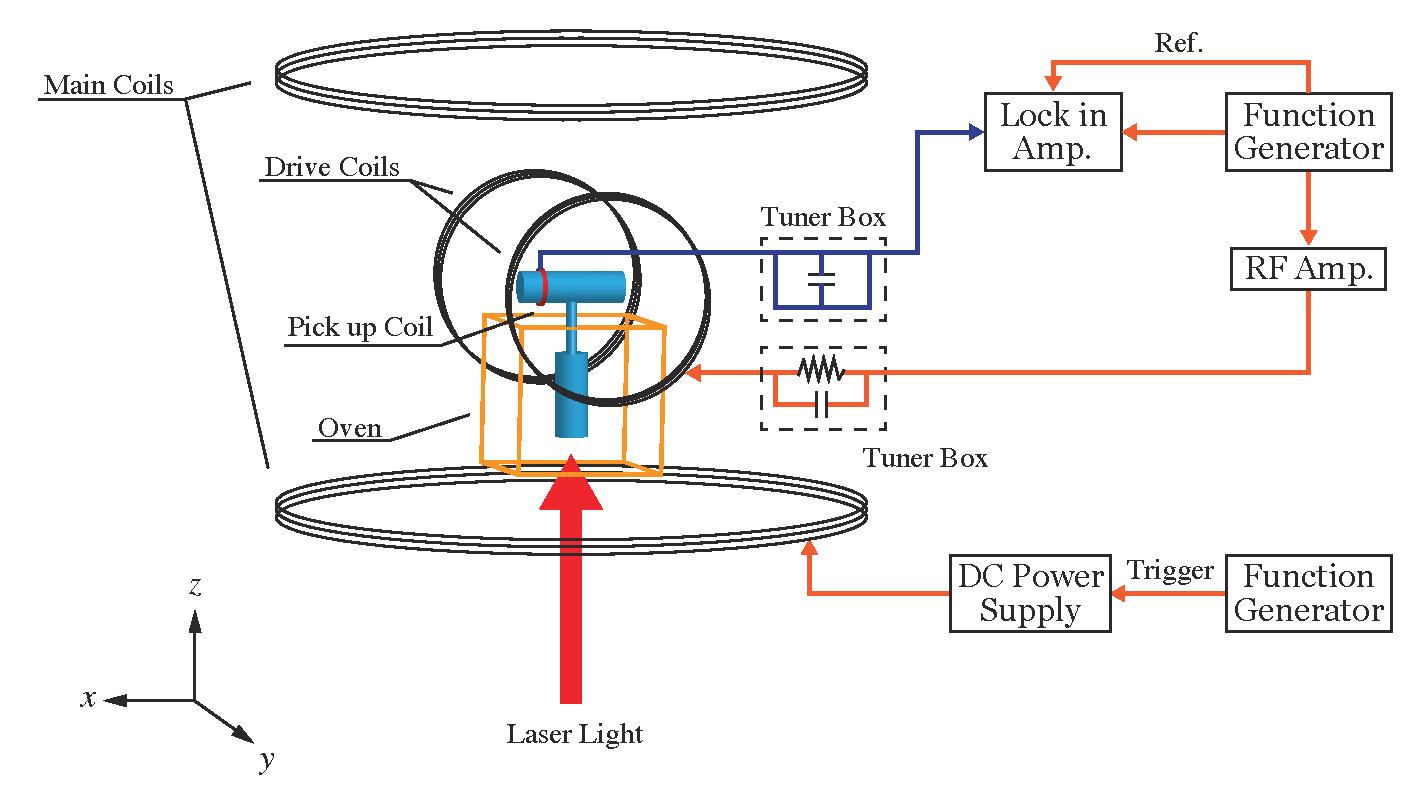
\includegraphics[clip, width=1.0\linewidth]{./chap3/fig/AFP-NMR_setup.pdf}\\
%  \caption{AFP-NMR装置の概略図}
%  \label{AFP-NMR}
% \end{figure}

% \begin{description}
%  \item[高周波磁場発生装置] \\
%  高周波磁場発生装置は、ファンクションジェネレーター(FG120, YOKOGAWA社)から出力された交流信号をRFアンプ(T145-4016A, THAMWAY社)によって増幅し、共振回路を通ってドライブコイルに印加することで高周波磁場を発生させる。\\
%  ドライブコイルは、標的セル周辺において均一な磁場を生成するために、メインコイルおよび補正コイルと同様にヘルムホルツ型のコイルとした。本研究におけるドライブコイルの仕様を表\ref{drive-coil_design}に示す。
% %
% \begin{table}[htbp]
%  \caption{本研究で使用したドライブコイルの仕様}
%  \centering
%   \begin{tabular}{|c|c|} \hline 
% 直径 & $45~{\rm cm}$ \\
% 導線の太さ & $\phi 1~{\rm mm}$ \\
% 巻き数 & $50$回 \\
% 抵抗 & $3.4~{\rm \Omega}$ \\
% インダクタンス & $6.1~{\rm mH}$ \\ \hline
%   \end{tabular}
%  \label{drive-coil_design}
% \end{table}
% %
% またドライブコイルの軸方向における磁場の大きさとドライブコイルに印加した直流電流との関係を図\ref{drive-coil}に示す。図\ref{drive-coil}のグラフは一次関数でフィッティングした結果を示しており、切片は測定した環境中の残留磁場によるものである。フィッティングの結果、ドライブコイルに流れる電流$I_{\rm drive}$と中心部におけるドライブコイルが作る磁場の大きさ$B_0$は
% %
% \begin{equation}
%  B_0~[{\rm mT}] = (0.203 \pm 0.010) \times I_{\rm drive}~[{\rm A}] + (0.056 \pm 0.006)
%  \label{B0-Idrive}
% \end{equation}
% %
% と表される。

% \begin{figure}[htbp]
%  \centering
%  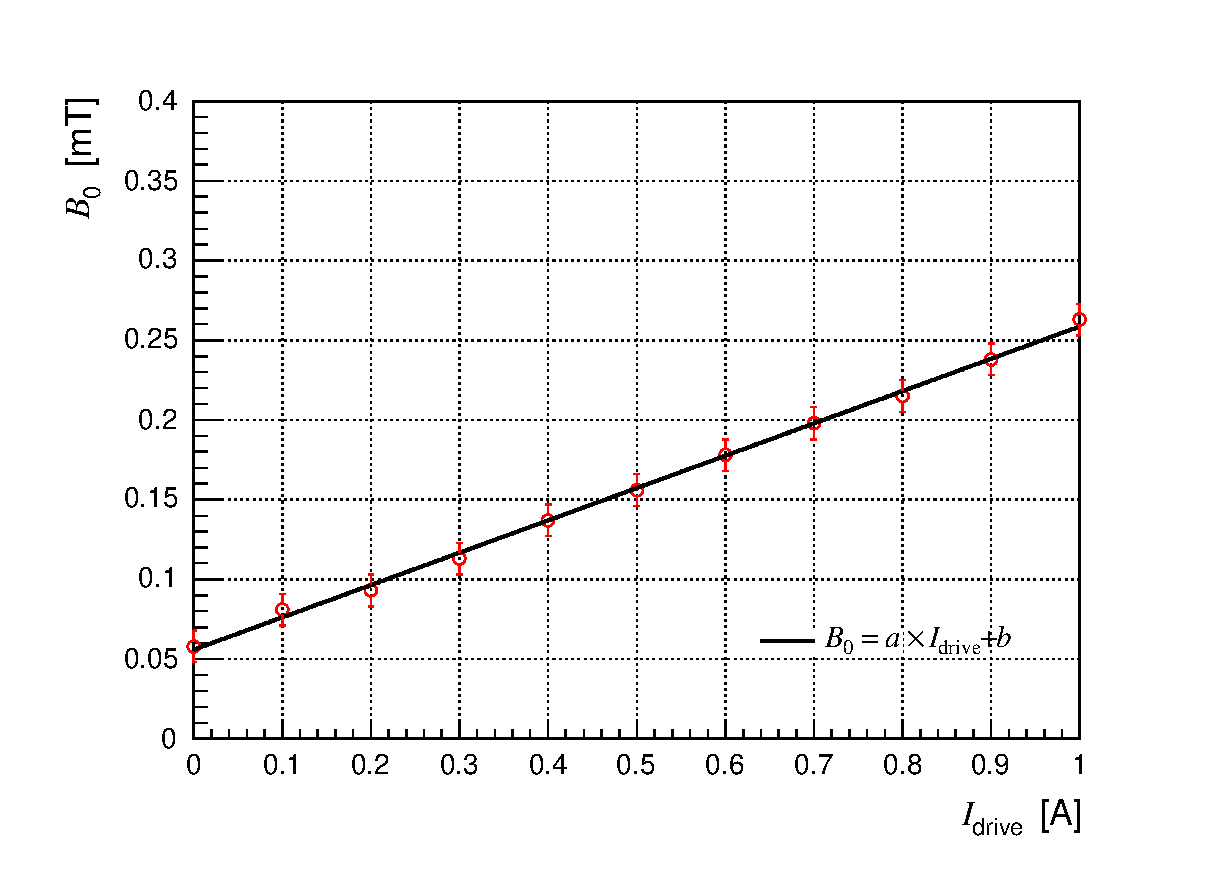
\includegraphics[clip, width=10cm]{./chap3/fig/Drive_Coil.eps}\\
%  \caption{ドライブコイルの励磁曲線}
%  \label{drive-coil}
% \end{figure}

%  メインコイルによって生成される静磁場の大きさは$1~{\rm mT}$程度なので、AFP条件からドライブコイルによって生成する振動磁場の振幅は$0.005〜0.010~{\rm mT}$程度が求められる。図\ref{drive-coil}におけるフィッティングの結果より、残留磁場の影響を無視すると、$0.005~{\rm mT}$程度の振幅を得るのに必要な印加電流はおよそ$25~{\rm mA}$となる。この条件を満たすために、ファンクションジェネレーターの出力信号をRFアンプおよび共振回路によって増幅させた。共振回路はドライブコイルに対して直列にコンデンサを入れた、直列共振回路(ドライブコイル用Tuner Box)を製作した。また印加電流値を読み取るために$10~{\rm \Omega}$の抵抗も組み込んだ。直列共振回路における共振周波数$f_0$は、次の式で書ける。
% %
% \begin{equation}
%  f_0 = \frac{\omega_0}{2 \pi} = \frac{1}{2 \pi \sqrt{LC}}
%  \label{series_reso}
% \end{equation}
% %
% ここで、$\omega_0$は共振角周波数、$L$はコイルのインダクタンスであり、$C$はコンデンサの電気容量である。仮に静磁場の大きさを$2.50~{\rm mT}$とした場合、式(\ref{B0_reso})よりNMRの共鳴周波数は
% %
% \begin{equation}
%  f_0 = \frac{2.50 \cdot 2.04 \times 10^5}{2 \pi} \simeq 81.2~[{\rm kHz}]
% \end{equation}
% %
% となる。式(\ref{series_reso})より、この共鳴周波数を得るために必要なコンデンサの電気容量は、表\ref{drive-coil_design}よりドライブコイルのインダクタンスが$L=6.1~{\rm mH}$であるから
% %
% \begin{eqnarray}
%  C &=& \frac{1}{(2 \pi f_0)^2 L} \nonumber \\
%  &=& \frac{1}{(2 \pi \cdot 81.2 \times 10^3)^2 \cdot 6.1 \times 10^{-3}} \nonumber \\
%  &\simeq& 0.630~[{\rm nF}]
% \end{eqnarray}
% %
% と求められる。実際は、回路系に含まれる浮遊容量等の影響があるので、計算値とは異なる値になると考えられる。\\
%  本研究で使用したドライブコイル用のTuner Boxの共振周波数測定結果を図\ref{drive-coil_tune}に示す。共振周波数の測定は、ドライブコイルに印加する電流の周波数を$0.5~{\rm kHz}$ずつ変化させつつ、Tuner Boxに組み込んだ抵抗の両端の電圧を読み取ることで行った。ファンクションジェネレーターの出力は$100~{\rm mV}$であり、コンデンサの電気容量は$0.253~{\rm nF}$とした。測定結果から、およそ$87~{\rm kHz}$の周波数において$25~{\rm mA}$以上の印加電流値が得られた。

% \begin{figure}[htbp]
%  \centering
%  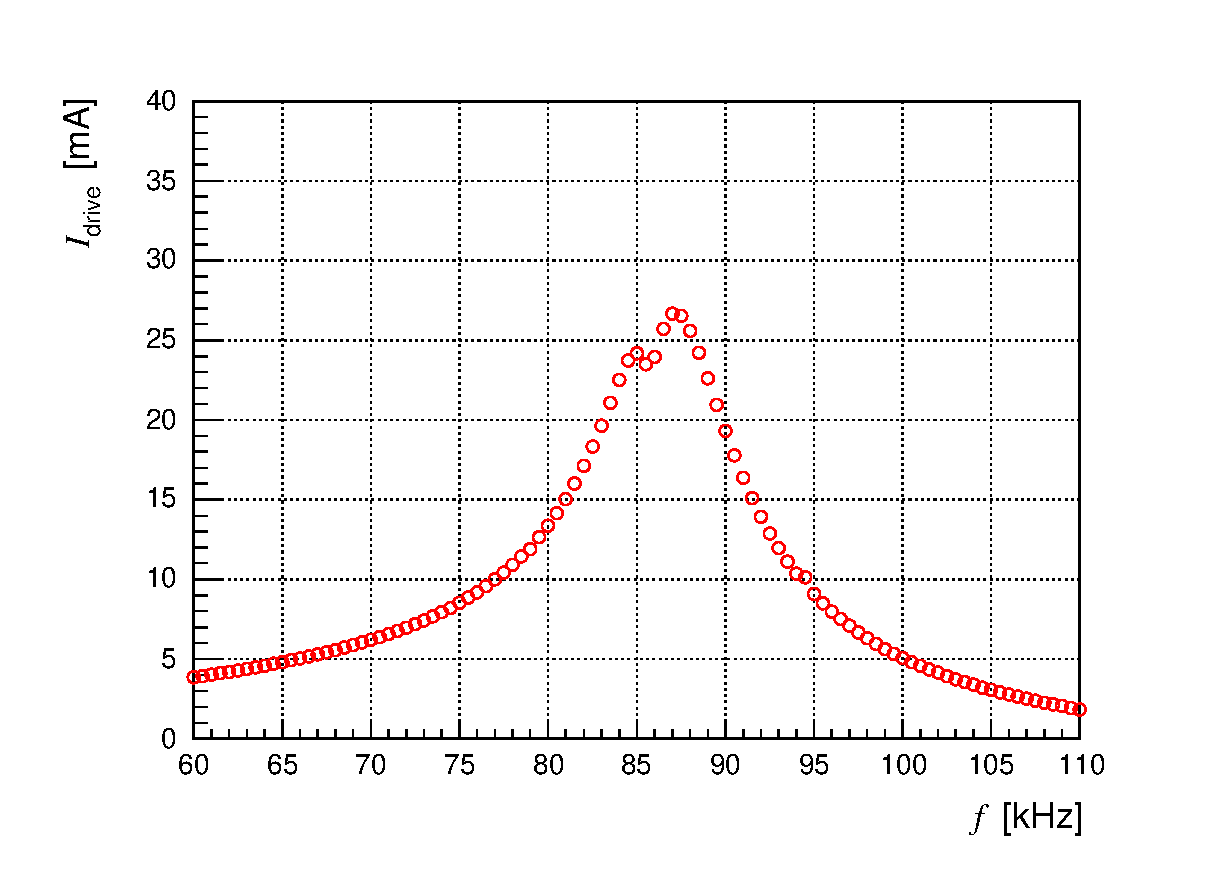
\includegraphics[clip, width=10cm]{./chap3/fig/Drive_Coil_tune.eps}\\
%  \caption{ドライブコイルの共振周波数測定。縦軸は実効値である。}
%  \label{drive-coil_tune}
% \end{figure}


%  \item[静磁場発生および掃引装置] \\
%  静磁場は、直流電源を用いてメインコイルに数 A程度の電流を流すことで発生させる。典型的な静磁場の大きさは$1〜3~{\rm mT}$である。今回使用した直流電源は、3.2.1節でも述べたようにTTL規格のトリガー信号を入力することで設定された二つの電流値の間を掃引できる。本研究では、ファンクションジェネレーターから$5~{\rm V}$のトリガー信号を直流電源に入力することで掃引を行った。また、ダイヤルによって磁場掃引時間を調整することができ、AFP条件を満たすような磁場の掃引速度を決定できる。本研究では磁場の掃引範囲として電流値を$2.50~{\rm A}$〜$5.95~{\rm A}$と設定した。これは磁場では$1.24~{\rm mT}$〜$2.96~{\rm mT}$に相当する。また掃引速度は、$1$秒あたり$0.19~{\rm A}$と設定した。

%  \item[NMR信号検出装置] \\
%  NMR信号検出装置は、偏極した$^3$He原子核集団が作る磁化を検出するためのピックアップコイル、信号を読み取るロックインアンプ(SR830, Stanford Research Systems社)、およびロックインアンプへ参照信号を入力するファンクションジェネレーターから構成される。\\
%  本研究で使用したピックアップコイルの仕様を表\ref{pick-coil_design}に示す。コイルの導線には$\phi 0.2~{\rm mm}$のエナメル線を使用し、$55$回巻きを四層重ねた$220$回巻きとした。また偏極した$^3$He原子核集団が作る磁化によってコイルに誘起される誘導電流を検出するために、回路系で得られる電圧が最大となるようにコンデンサを並列に組み込んだ並列共振回路(ピックアップコイル用Tuner Box)を製作した。コンデンサの電気容量は$0.08~{\rm nF}$とし、ドライブコイル用のTuner Boxと同様に共振周波数測定を行った。測定結果を図\ref{pick-coil_tune}に示す。この時、ピックアップコイルはドライブコイルと平行になるように設置し、ファンクションジェネレーターの出力は$100~{\rm mV}$とした。また測定時はドライブコイル用のTuner Boxを取り外し、抵抗のみを入れたものを組み込んだ。これにより、ドライブコイルに流れる電流が周波数に依らずほぼ一定となる。測定結果から、およそ$86~{\rm kHz}$において共振ピークが得られた。
% %
% \begin{table}[htbp]
%  \caption{ピックアップコイルの仕様}
%  \centering
%   \begin{tabular}{|c|c|} \hline 
% 直径 & $46~{\rm mm}$ \\
% 導線の太さ & $\phi 0.2~{\rm mm}$ \\
% 巻き数 & $220$回 \\
% 抵抗 & $21~{\rm \Omega}$ \\
% インダクタンス & $3.6~{\rm mH}$ \\ \hline
%   \end{tabular}
%  \label{pick-coil_design}
% \end{table}
% %

% \begin{figure}[tbp]
%  \centering
%  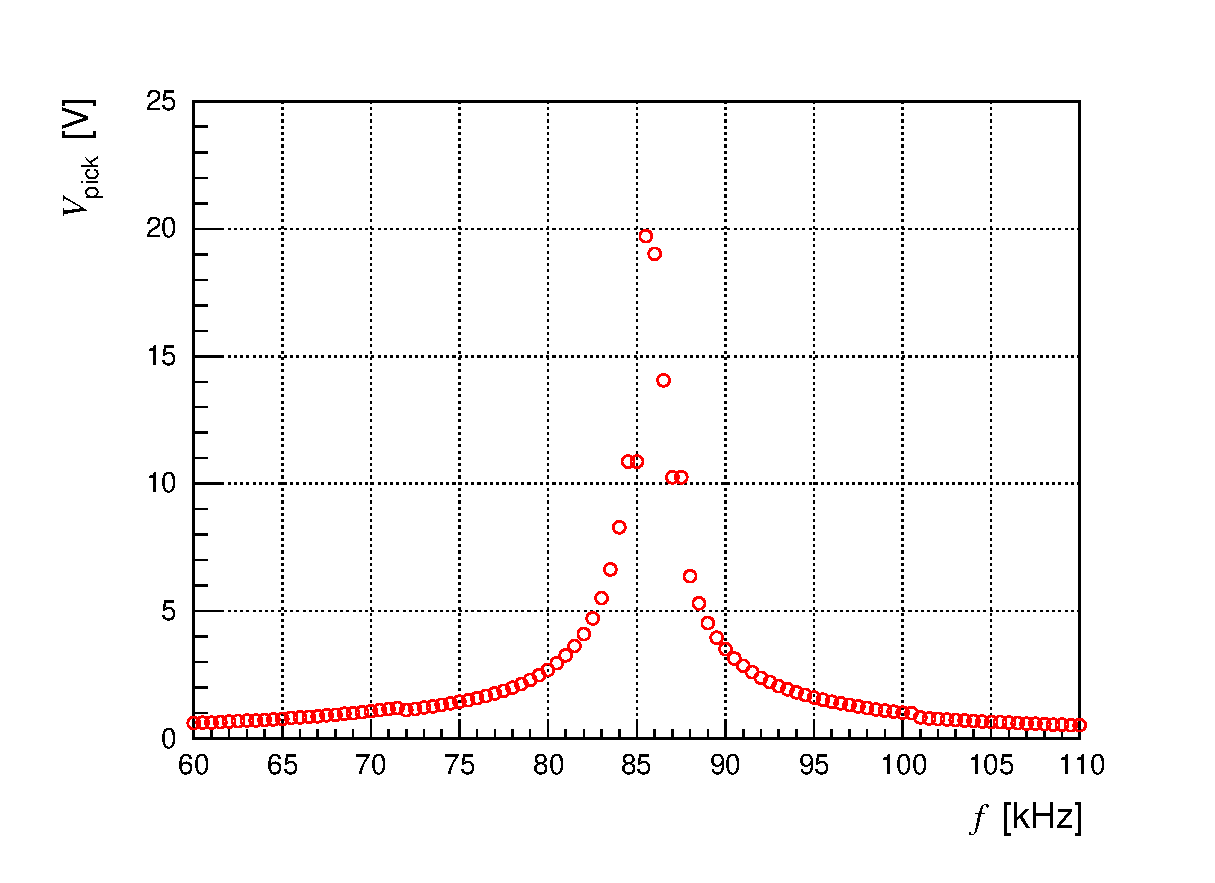
\includegraphics[clip, width=10cm]{./chap3/fig/Pickup_Coil_tune.eps}\\
%  \caption{ピックアップコイルの共振周波数測定。縦軸は実効値である。}
%  \label{pick-coil_tune}
% \end{figure}

%  ピックアップコイルに誘起されたNMR信号は、ロックインアンプを用いて測定した。ロックインアンプは特定の周波数成分の信号を取り出して増幅できる機器であり、ノイズに埋もれるような微小信号を非常に高感度で検出できる。これにより、式(\ref{V_pick})で表されるピックアップコイルに誘起される電圧の$\cos(\omega t)$の成分のみを取り出すことができる。以下に、ロックインアンプの測定原理について述べる。\\
%  ロックインアンプで取得したい信号$V_{\rm sig}(t)$を
% %
% \begin{equation}
%  V_{\rm sig}(t) = V_{\rm sig}^0 \cos(\omega_{\rm sig}t + \phi_{\rm sig})
%  \label{V_sig}
% \end{equation}
% %
% のように、周波数$\omega_{\rm sig}$をもつ周期関数とする。一般に、ロックインアンプへの入力信号には取得したい信号以外のバックグラウンドも含まれる。この取得したい信号に対し、ロックインアンプに参照信号として
% %
% \begin{equation}
%  V_{\rm ref}(t) = V_{\rm ref}^0 \cos(\omega_{\rm ref}t + \phi_{\rm ref})
%  \label{V_ref}
% \end{equation}
% %
% を入力する。ロックインアンプに入力された参照信号は、$90^\circ$位相シフト回路によって
% %
% \begin{eqnarray}
%  V_{\rm ref}^x(t) &=& V_{\rm ref}^0 \cos(\omega_{\rm ref}t + \phi_{\rm ref}) \\
%  V_{\rm ref}^y(t) &=& V_{\rm ref}^0 \sin(\omega_{\rm ref}t + \phi_{\rm ref})
% \end{eqnarray}
% %
% の二つの成分($x$成分および$y$成分)に分けられる。参照信号のこれらの成分を入力信号と積算させることにより
% %
% \begin{eqnarray}
%  V_x'(t) &=& V_{\rm sig}^0 \cos(\omega_{\rm sig}t + \phi_{\rm sig}) \times V_{\rm ref}^0 \cos(\omega_{\rm ref}t + \phi_{\rm ref}) \nonumber \\
%  &=& \frac{1}{2}V_{\rm sig}^0V_{\rm ref}^0 \{ \cos[(\omega_{\rm sig}-\omega_{\rm ref})t + (\phi_{\rm sig}-\phi_{\rm ref})] \nonumber \\
%  & & + \cos[(\omega_{\rm sig}+\omega_{\rm ref})t + (\phi_{\rm sig}+\phi_{\rm ref})] \}
% \end{eqnarray}
% %
% %
% \begin{eqnarray}
%  V_y'(t) &=& V_{\rm sig}^0 \cos(\omega_{\rm sig}t + \phi_{\rm sig}) \times V_{\rm ref}^0 \sin(\omega_{\rm ref}t + \phi_{\rm ref}) \nonumber \\
%  &=& \frac{1}{2}V_{\rm sig}^0V_{\rm ref}^0 \{ \sin[(\omega_{\rm sig}+\omega_{\rm ref})t + (\phi_{\rm sig}+\phi_{\rm ref})] \nonumber \\
%  & & - \sin[(\omega_{\rm sig}-\omega_{\rm ref})t + (\phi_{\rm sig}-\phi_{\rm ref})] \}
% \end{eqnarray}
% %
% となり、低周波(周波数:$\omega_{\rm sig}-\omega_{\rm ref}$)成分と高周波(周波数:$\omega_{\rm sig}+\omega_{\rm ref}$)成分をもつ直交した信号$V_x'(t)$および$V_y'(t)$が得られる。またロックインアンプにはローパスフィルターが内蔵されており、これによって高周波成分はキャンセルされる。よって、$\omega_{\rm sig} = \omega_{\rm ref}$となるような参照信号を用いることにより
% %
% \begin{eqnarray}
%  V_x &=& \frac{1}{2}V_{\rm sig}^0V_{\rm ref}^0 \cos(\phi_{\rm sig} - \phi_{\rm ref}) \\
%  V_y &=& -\frac{1}{2}V_{\rm sig}^0V_{\rm ref}^0 \sin(\phi_{\rm sig} - \phi_{\rm ref})
% \end{eqnarray}
% %
% のような直流電圧が得られる。また位相差$\phi_{\rm sig} - \phi_{\rm ref}$による影響を無くすために
% %
% \begin{equation}
%  V_R \equiv \sqrt{V_x^2 + V_y^2} = \frac{1}{2}V_{\rm sig}^0V_{\rm ref}^0
%  \label{V_R}
% \end{equation}
% %
% を演算することによって、位相差に依らない直流信号を得ることができる。以上の原理により、ピックアップコイルに誘起される偏極した$^3$He原子核集団が作る磁化起因のNMR信号を測定できる。

% \end{description}

% %%%%%%%

% %% 3.3.2 %%
%   \subsection{Rb-ESR測定装置}
% AFP-NMR法による測定のみでは、$^3$He偏極度の絶対値を求めることができない。そこで本研究では、AFP-NMR測定における$^3$He偏極度の絶対値較正を行うために、RbのESR周波数シフト測定による$^3$He偏極度測定システムを開発した。\\
%  RbのESR周波数シフト測定を行うためのRb-ESR測定装置の概略図を図\ref{Rb-ESR}に示す。標的オーブン内に設置されたESRコイルによって標的セルのポンピング部に振動磁場をかけてESRを誘起し、それによって光ポンピングにより励起されたRb原子を脱励起させる。その際に放出する$D_2$線($780~{\rm nm}$)をフォトダイオード(S2387-1010R, 浜松ホトニクス社)で観測することで、RbのESR測定を行う。この時、$D_2$線のみを観測するためにフォトダイオードの受光面の前面に$D_2$フィルター(VPFHT-12.5C-7800, シグマ光機社)を入れた。このフィルターの中心波長は$780~{\rm nm}$で、半値幅は$4.25~{\rm nm}$である。これにより、光ポンピングの円偏光レーザー(795~{\rm nm})の反射光等を遮断する。またフォトダイオードの信号はI-V変換器(T-IVA001BZ, TURTLE社)によって増幅させ、ロックインアンプに入力した。

% \begin{figure}[tbp]
%  \centering
%  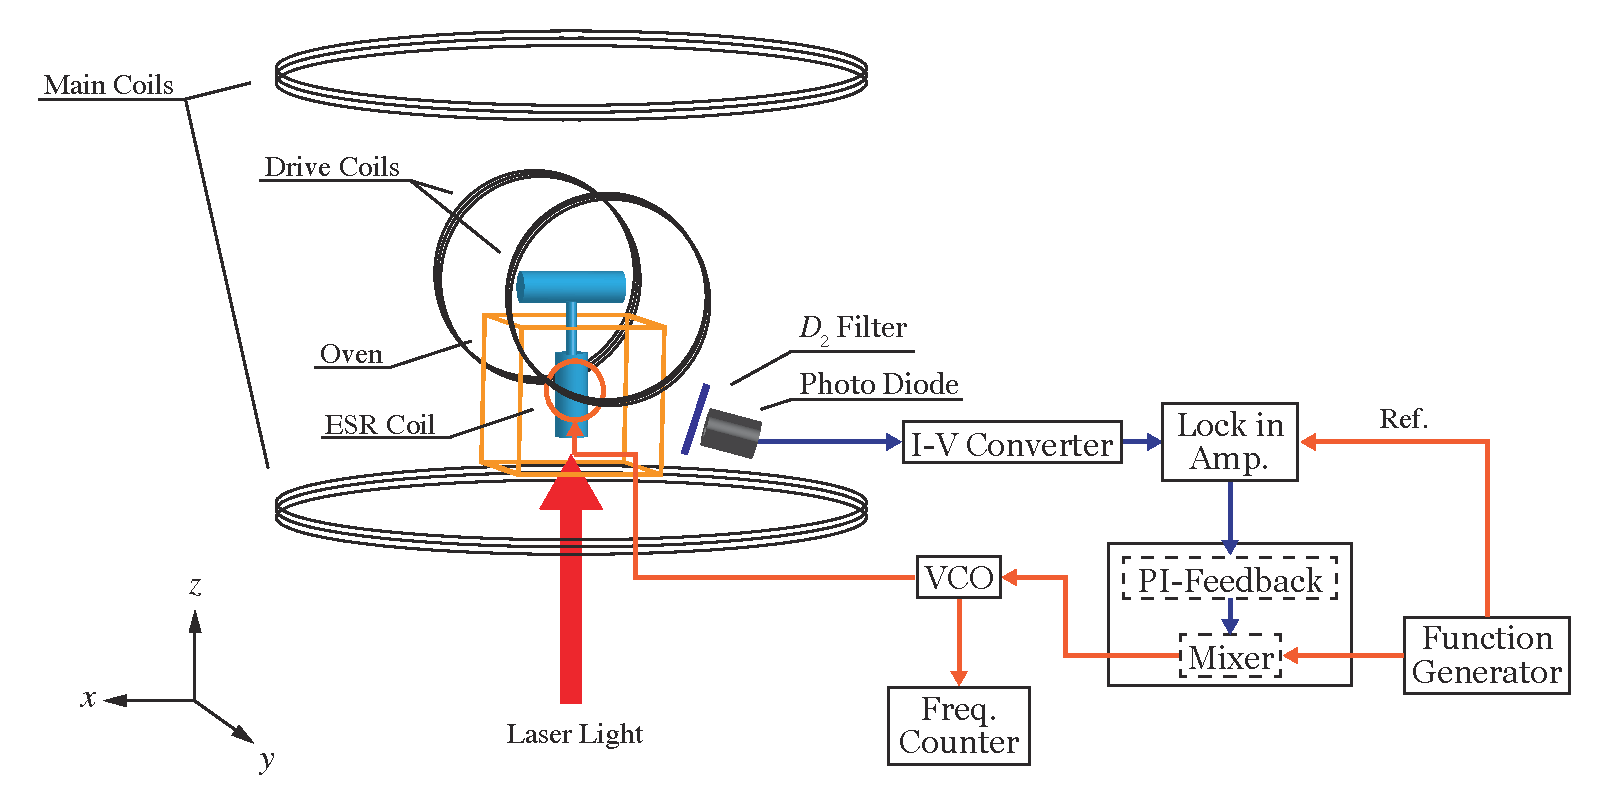
\includegraphics[clip, width=1.0\linewidth]{./chap3/fig/ESR_setup.pdf}\\
%  \caption{Rb-ESR測定装置の概略図}
%  \label{Rb-ESR}
% \end{figure}

% 振動磁場を印加するESRコイルは電圧制御発振器(VCO)に接続されている。VCOは入力信号の大きさに応じて発振する信号の周波数を制御できるもので、本研究ではVCOとしてHEWLETT PACKARD社製のHP8116Aを用いた。VCOへの制御入力信号としてsin波と直流電圧(offset)を用いることで、ESR周波数の前後で振動磁場の周波数を変調させることができる。本測定では、制御入力信号としてファンクションジェネレーター(33220A, Agilent社)の出力を用いた。出力するsin波の振幅は$60~{\rm mVpp}$、変調周波数は$120~{\rm Hz}$とした。またoffsetは$3~{\rm V}$程度とした。\\
%  ESR周波数は静磁場の大きさに依存するので、磁場のふらつきによってESR周波数もふらつくことが考えられる。そこで、振動磁場の周波数を常にESR周波数を中心として変調させるために、PI-フィードバック回路を組み込んだ。フォトダイオードの信号をロックインアンプに入力し、また参照信号として振動磁場と同様の周波数を持つ矩形波もファンクションジェネレーターからロックインアンプに入力する。この時のロックインアンプの$y$出力$V_y$を、ESR周波数からのずれを反映する信号としてPI-フィードバック回路へと入力し、適当な時定数で増幅させてミキサーへ入力する。ミキサーにはファンクションジェネレーターのsin波信号も入力されており、PI-フィードバック回路からの信号をこれに加えてVCOへと制御信号として入力する。振動磁場の周波数がESR周波数となっていれば$V_y=0$となるが、ESR周波数からずれていれば$V_y \neq 0$となる。振動磁場の周波数がESR周波数よりも低周波数側にずれた時は正のフィードバックを、高周波数側にずれた時は負のフィードバックをかけることで、振動磁場の周波数が常にESR周波数を中心として変調される。またこの時の振動磁場の周波数は、VCOの出力を周波数カウンター(TR5822, ADVANTEST社)に入力して測定した。周波数カウンターをLinuxコンピューターのGPIB制御によって動作させ、測定データをPCに取り込んだ。

% %%%%%%%
% %%%%%%%%%%

 \chapter{考察}
\section{緩和項の相対評価}
\begin{figure}[h]
  \centering
  \includegraphics[width=10cm]{./chap4/fig/comparison.png}
  \caption{ビーム照射中の緩和効果の比較}
\end{figure}
(グラフは和の形で表記していることがわかるように修正する)
レーザ照射下の偏極緩和項は加速器によるビーム照射の有無にかかわらず存在する。
\\
$\downarrow \bf{この部分はわかりにくいので後ほど書き直す}$\\
・強度効果を定数にした話(多くの仮定をしているので単純に今回はこう考えました、という話)\\
強度効果による緩和項は微分方程式中で定数で置いていたため、グラフ中でもビーム照射中のみ一定に寄与している。
本論文では強度効果は結晶温度に比例すると仮定している。
結晶温度はナフタレンの比熱とビームから与えられた熱量の積となる。
ナフタレンの比熱と温度は図$\ref{C_T}$のような関係を持つことがわかっており$\cite{Chem}$、$0 [K]<T<273 [K]$の範囲で比例関係にあるとみなすことができる。
したがって、ビーム照射により一定の熱量を与え続けた場合、標的温度の上昇に伴いナフタレンの温度上昇に必要な熱量も増加し、ある時点で温度は平衡に達すると考えた。
温度が平衡に達すると強度効果も固定値となるため、温度が平衡に達するまでの上昇を$\rm{exp}(\frac{t}{\gamma})$として補正したうえで強度効果を定数として微分方程式に取り込んだ。
ただし、本論文ではビーム強度によって達する平衡温度と平衡に達するまでの時間が異なることを考慮できていないため、今後改善が必要である。
\begin{figure}[h]
  \centering
  \includegraphics[width=10cm]{./chap4/fig/C_T.png}
  \caption{ナフタレンの飽和圧力におけるモル熱容量$\cite{Chem}$}
  \label{C_T}
\end{figure}


\section{長時間・大強度ビーム照射時の減偏極予想}
\begin{figure}[h]
  \centering
  \includegraphics[width=10cm]{./chap4/fig/longtime.png}
  \caption{長時間・大強度ビーム照射時の減偏極予想}
\end{figure}
本論文における最適パラメータを用いて、各ビーム強度で長時間ビーム照射を行った時の減偏極の様子を計算した。
このグラフと先ほどの緩和項比較のグラフから、長時間ビーム照射時の減偏極は積分項の効果が支配的となることがわかる。
また、ビーム強度$1 \times 10^7$ [cps]以上では24時間で偏極度が5割を下回ると推定できる。
今後のビーム照射試験時はビーム強度および照射時間を設定する際にこれらの推定が判断材料となると考えられる。


% \chapter{${}^3$Heの偏極生成と偏極度の絶対値較正}
% 第3章で述べた偏極$^3$He標的装置を用いて、$^3$Heの偏極生成および$^3$He偏極度測定を行った。またRbのESR周波数シフト測定を行い、$^3$He偏極度の絶対値を求めるとともに、AFP-NMR法により得られるNMR信号の較正を行った。本章では、それらの測定結果について述べる。

% %%%% 4.1 %%%%
%  \section{${}^3$He偏極生成}
% 本研究での$^3$He偏極生成には、標的セル製作装置で製作したKukiセルを用いた。$^3$Heの偏極生成では、オーブン温度を$160$℃に設定し、レーザー出力$20~{\rm W}$で光ポンピングを行った。3.2.3節で述べたように、本研究で用いた半導体レーザーは最大出力が$30~{\rm W}$であるが、ファイバー端の部分での発熱が確認されたため、安全面を考慮し出力を少し落として光ポンピングを行った。\\
%  $^3$Heの偏極生成の時間変化は、1時間毎にNMR測定を行うことで確認した。NMR測定時の測定系の条件を表\ref{NMR_cond}に示す。
% %
% \begin{table}[htbp]
%  \caption{NMRの測定条件}
%  \centering
%   \begin{tabular}{|c|c|} \hline
% 項目 & 設定値 \\ \hline \hline
% 静磁場掃引範囲 & $1.24~{\rm mT}$〜$2.96~{\rm mT}$ \\
% 掃引速度$dB/dt$ & $0.095~{\rm mT/s}$ \\
% RF周波数$f$ & $87.0~{\rm kHz}$ \\
% 共鳴磁場$B_0$ & $2.68~{\rm mT}$ \\
% RFの大きさ$B_1$ & $2.5 \times 10^{-3}~{\rm mT}$ \\ \hline 
%   \end{tabular}
%  \label{NMR_cond}
% \end{table}
% %

% %% 4.1.1 %%
%   \subsection{偏極発展}
% 光ポンピングによる$^3$He偏極度の時間変化(偏極発展)は、式(\ref{P_3He_final})で示したように
% %
% \begin{equation}
%  {P}_{\rm ^3He} = \overline{P}_{\rm Rb} \frac{\gamma_{\rm SE}}{\gamma_{\rm SE}+\Gamma_{\rm ^3He}} \left[ 1-e^{-(\gamma_{\rm SE}+\Gamma_{\rm ^3He})t} \right]
%  \label{P_3He_final2}
% \end{equation}
% %
% と書ける。また十分時間が経過した時($t \to \infty$)の$^3$He原子核の偏極度$\overline{P}_{\rm ^3He}$は、$X$-factorを考慮すると式(\ref{P_3He_X})で示したように
% %
% \begin{eqnarray}
%  \overline{P}_{\rm ^3He} &=& \overline{P}_{\rm Rb} \frac{\gamma_{\rm SE}}{\gamma_{\rm SE}(1+X)+\Gamma_{\rm ^3He}} \nonumber \\
%  &=& \overline{P}_{\rm Rb} \frac{\gamma_{\rm SE}}{\gamma_{\rm SE}+\Gamma_{\rm ^3He}'} 
%  \label{P_3He_X2}
% \end{eqnarray}
% %
% となる。ここで、$\Gamma_{\rm ^3He}' = X \cdot \gamma_{\rm SE}+\Gamma_{\rm ^3He}$はRb蒸気と$^3$He原子核との相互作用も考慮した$^3$He原子核の偏極緩和率である。また偏極発展における立ち上がりの時定数$\tau_{\rm build}$は、
% %
% \begin{equation}
%  \tau_{\rm build} = \frac{1}{\gamma_{\rm SE}+\Gamma_{\rm ^3He}'}
%  \label{tau_build}
% \end{equation}
% %
% と表される。よって$^3$Heの偏極発展を測定し、$\tau_{\rm build}$の値が求まれば、Rb原子と$^3$He原子核のスピン交換率$\gamma_{\rm SE}$および$^3$He原子核の偏極緩和率$\Gamma_{\rm ^3He}'$の和を求めることができる。\\
%  Kukiセルを用いた場合の典型的な$^3$Heの偏極発展の測定結果を図\ref{NMR_build}に示す。図\ref{NMR_build}における実線は、図中に示された式(式(\ref{P_3He_final2})と同様の形)でフィッティングした結果である。また3.1節で述べたように、今回使用したKukiセルはポンピング部と、NMR信号を検出するためのピックアップコイルが設置されている標的部をもつダブルセル構造である。よって、偏極発展を開始してから偏極した$^3$He原子核が標的部に達するまでに時間差が生じる。故に、厳密には偏極発展開始直後における$^3$He偏極度の時間変化は式(\ref{P_3He_final2})と一致しない。以上の理由から、図\ref{NMR_build}の$t \sim 0.5~{\rm h}$における点はフィッティングの範囲に含めないようにした。フィッティングの結果、到達信号強度$V_{\rm max}$および発展の時定数$\tau_{\rm build}$は
% %
% \begin{eqnarray}
%  V_{\rm max} &=& 204.3 \pm 3.4~[{\rm mV}] \\
%  \tau_{\rm build} &=& 7.43 \pm 0.36~[{\rm h}]
% \end{eqnarray}
% %
% となった。

% \begin{figure}[tbp]
%  \centering
%  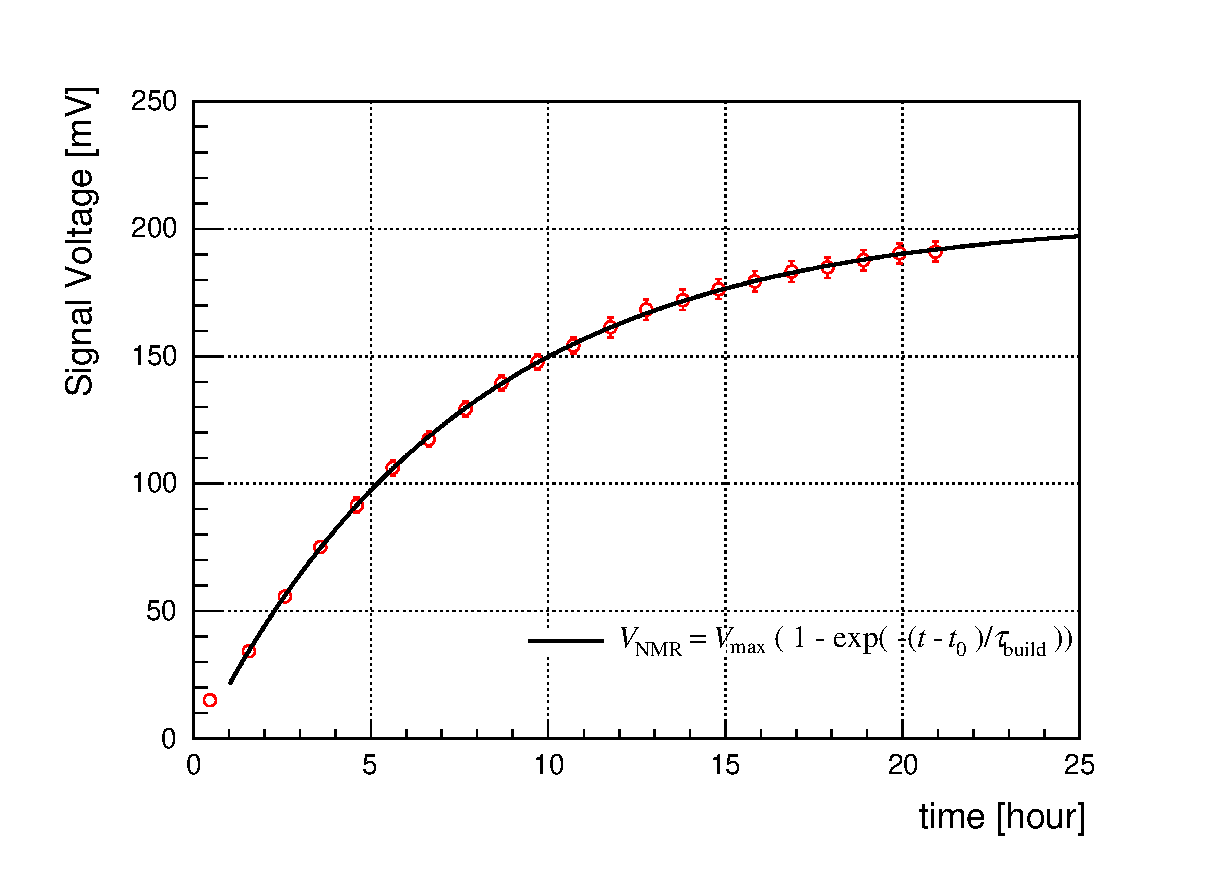
\includegraphics[clip, width=10cm]{./chap4/fig/NMR-buildup_1230.eps}\\
%  \caption{Kukiセルでの$^3$Heの偏極発展}
%  \label{NMR_build}
% \end{figure}


% %%%%%%%

% %% 4.1.2 %%
%   \subsection{偏極緩和}
% オーブンの温度を高温に保ちつつ、光ポンピングによって$^3$He原子核が偏極している状態でレーザーの照射を止めると、$^3$He原子核は偏極生成されなくなるために次第に偏極度が減少していく(偏極緩和)。光ポンピングがされなくなると、Rb原子の偏極は$^3$He原子核の偏極より十分速く緩和する。よって、$^3$He原子核の偏極度の時間変化(式(\ref{dP_3He/dt}))において$\overline{P}_{\rm Rb}=0$と見なせる。故に、この時の$^3$He原子核の偏極度は、次の式で書ける。
% %
% \begin{equation}
%  P_{\rm ^3He} = P_0 e^{-\Gamma_{\rm ^3He}'t}
%  \label{relax_hot}
% \end{equation}
% %
% ここで、$P_0$は$t=0$の時の$^3$He偏極度である。この条件における偏極緩和(高温偏極緩和)の立ち下りの時定数$\tau_{\rm hot}$は、式(\ref{relax_hot})より
% %
% \begin{equation}
%  \tau_{\rm hot} = \frac{1}{\Gamma_{\rm ^3He}'} = \frac{1}{X \cdot \gamma_{\rm SE}+\Gamma_{\rm ^3He}}
%  \label{tau_hot}
% \end{equation}
% %
% となる。よって$^3$Heの偏極緩和を測定し、$\tau_{\rm hot}$の値が求まれば、Rb蒸気との相互作用も含んだ$^3$He原子核の偏極緩和率$\Gamma_{\rm ^3He}'$を求めることができる。\\
%  Kukiセルを用いた場合の典型的な$^3$Heの高温偏極緩和の測定結果を図\ref{NMR_hotrelax}に示す。図\ref{NMR_hotrelax}における実線は、式(\ref{relax_hot})でフィッティングした結果である。またこの時、$t=0~{\rm h}$におけるNMR信号の大きさを$1$とした。フィッティングの結果、高温偏極緩和における時定数$\tau_{\rm hot}$は
% %
% \begin{equation}
%  \tau_{\rm hot} = 7.93 \pm 0.14~[{\rm h}]
% \end{equation}
% %
% となった。

% \begin{figure}[tbp]
%  \centering
%  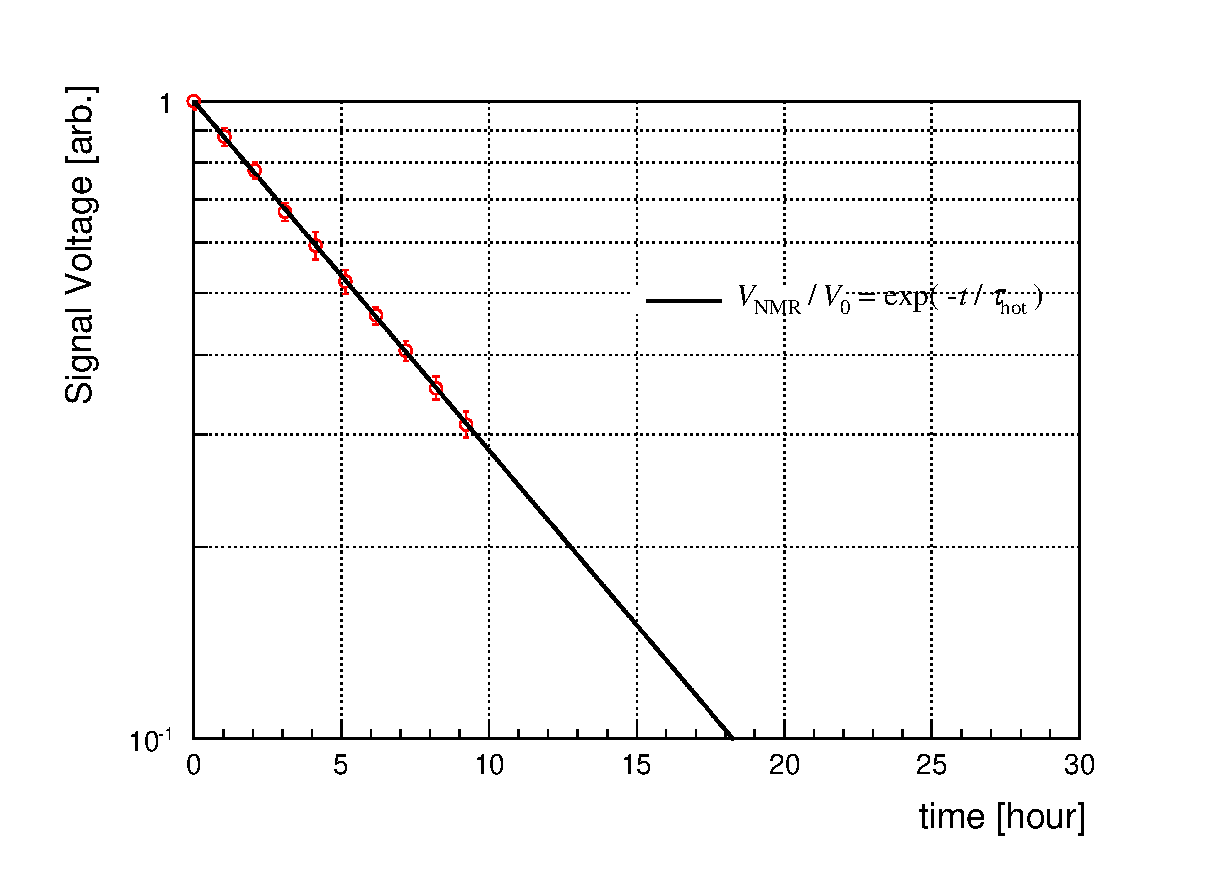
\includegraphics[clip, width=10cm]{./chap4/fig/NMR-hotrelax_1229.eps}\\
%  \caption{Kukiセルでの$^3$Heの高温偏極緩和}
%  \label{NMR_hotrelax}
% \end{figure}

% また光ポンピングによって$^3$He原子核が偏極している状態でレーザーの照射を止めると同時に、オーブンの加熱も止め、標的セル内の温度をRbの融点($39.31$℃)以下にすると、Rbが凝縮および凝固する。よって、Rb蒸気と$^3$He原子核との相互作用が無視できるようになる。この条件における偏極緩和(低温偏極緩和)の立ち下りの時定数$\tau_{\rm cold}$は
% %
% \begin{equation}
%  \tau_{\rm cold} = \frac{1}{\Gamma_{\rm ^3He}}
%  \label{tau_cold}
% \end{equation}
% %
% となり、Rb原子の数密度に依存しない$^3$He原子核の偏極緩和率を求めることができる。この低温偏極緩和における時定数$\tau_{\rm cold}$は、標的セル自体の性能を比較できるひとつの指標となる。\\
%  Kukiセルを用いた場合の典型的な$^3$Heの低温偏極緩和の測定結果を図\ref{NMR_coldrelax}に示す。図\ref{NMR_coldrelax}における実線は、式(\ref{relax_hot})と同様の形の式でフィッティングした結果である。またこの時、高温偏極緩和測定の場合と同様に$t=0~{\rm h}$におけるNMR信号の大きさを$1$とした。フィッティングの結果、低温偏極緩和における時定数$\tau_{\rm cold}$は
% %
% \begin{equation}
%  \tau_{\rm cold} = 9.73 \pm 0.11~[{\rm h}]
% \end{equation}
% %
% となり、高温偏極緩和の場合よりも$1.8~{\rm h}$程度長い緩和の時定数が得られた。よって、Rb蒸気と$^3$He原子核との相互作用による影響が無視されたことが確認できた。

% \begin{figure}[tbp]
%  \centering
%  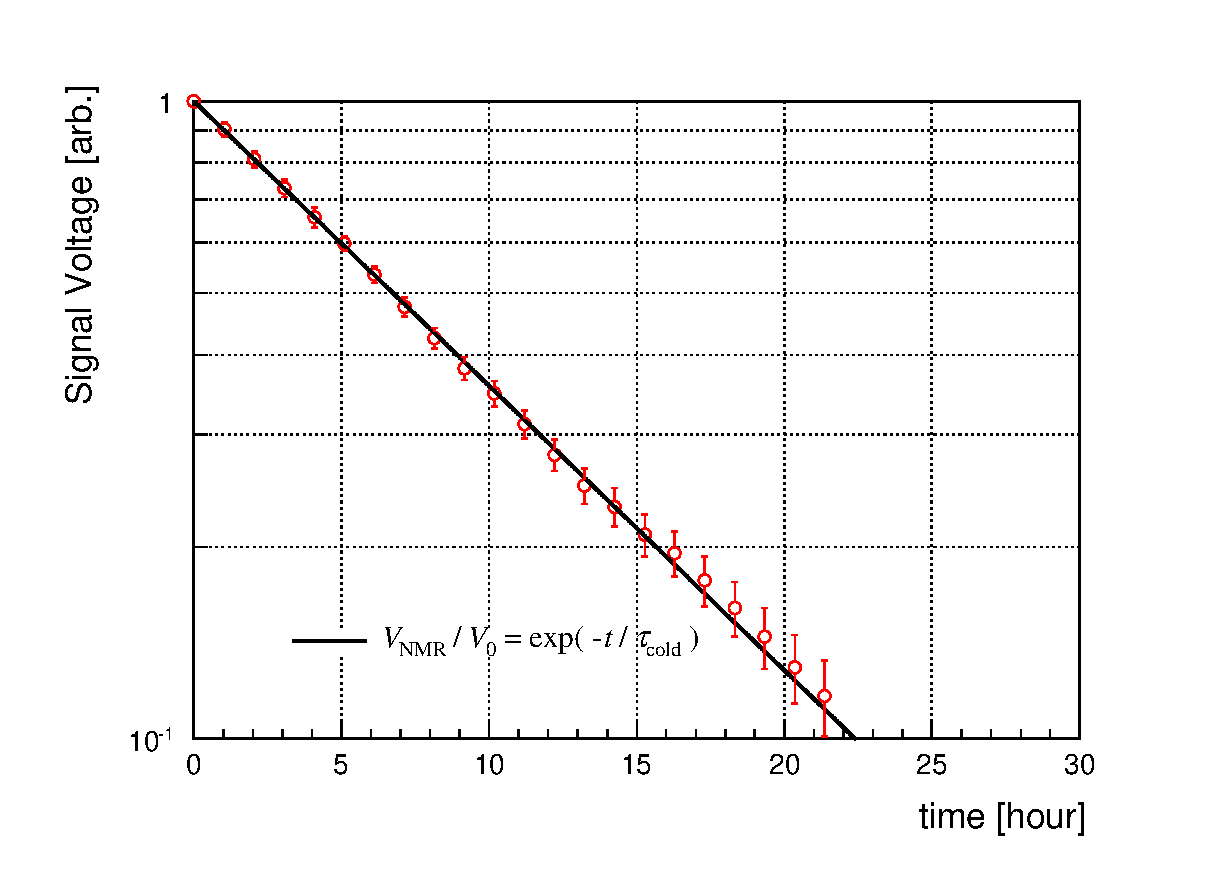
\includegraphics[clip, width=10cm]{./chap4/fig/NMR-coldrelax_1225.eps}\\
%  \caption{Kukiセルでの$^3$Heの低温偏極緩和}
%  \label{NMR_coldrelax}
% \end{figure}

 
% %%%%%%%

% %%%%%%%%%%

% %%%% 4.2 %%%%
%  \section{${}^3$He偏極度の絶対値較正}
% AFP-NMR法のみでは、$^3$He偏極度に比例した大きさのNMR信号しか得ることができない。$^3$He偏極度の絶対値を求めるために、第3章で述べたRbのESR周波数シフト測定による$^3$He偏極度測定システムを開発し、Rb-ESR測定装置を用いて$^3$He偏極度の測定を行った。以下の節では、$^3$He偏極度の測定結果およびNMR信号の較正について述べる。

% %% 4.2.1 %% 
%   \subsection{RbのESR周波数シフトによる${}^3$He偏極度測定}
% RbのESR周波数シフトは、$^3$He原子核の核スピンの向きが静磁場方向に対して平行または反平行それぞれにおけるRbのESR周波数を測定し、その差を取ることで得られる。$^3$He原子核の核スピンはAFP法によって反転させる。反転時にNMR測定も同時に行い、その時に得られたNMR信号を、RbのESR周波数シフトから求められる$^3$He偏極度に対応するものとする。\\
%  RbのESR周波数シフトの測定結果を図\ref{ESRfreq_mea}に示す。ESR周波数は、測定間隔$100~{\rm ms}$で$100$回測定(測定時間:$10$秒)を行うことで取得した。図\ref{ESRfreq_mea}において、$^3$He核スピンが上向き(静磁場に対して反平行)の場合は赤い三角、一方$^3$He核スピンが下向き(静磁場に対して平行)の場合は青い三角で示している。また、それぞれの点は10個毎に平均を取った値である。更に、図\ref{ESRfreq_mea}では偏極反転時に得られたNMR信号強度も示している。時間経過と共にNMR信号強度が減少し、それに従ってESR周波数シフトも小さくなっていることが分かる。これは円偏光のレーザーによる光ポンピングを測定中も行っているために、$^3$He原子核の核スピンの向きが静磁場と平行の時にレーザーによって$^3$Heの偏極を緩和(逆ポンピング)させていることによる。なるべく逆ポンピングによる$^3$He偏極度の緩和を抑制するために、一回のESR周波数の測定時間は$10$秒程度とした。測定結果から、およそ$2〜3~{\rm kHz}$程度のESR周波数シフトが得られた。

% \begin{figure}[tbp]
%  \centering
%  \includegraphics[clip, width=11cm]{./chap4/fig/ESRfreq_ave_Vnmr.eps}\\
%  \caption{典型的なESR周波数の測定データおよび偏極反転時のNMR信号強度}
%  \label{ESRfreq_mea}
% \end{figure}

% $\Delta \nu_{\rm ESR} = 3~{\rm kHz}$とした時の$^3$He偏極度を求める。RbのESR周波数シフト$\Delta \nu_{\rm ESR}$は、式(\ref{ESR_shift_updown})でも示したように
% %
%  \begin{eqnarray}
%   \Delta \nu_{\rm ESR}(m_F=\pm F) &=& \frac{2\mu_0}{3} \frac{\mu_{\rm B} g_e}{h(2I+1)} \left( 1\mp \frac{8I}{(2I+1)^2} \frac{\mu_{\rm B} g_e B_0}{hA_{\rm hfs}} \right)\kappa_0 \mu_{\rm K} [{\rm {}^3He}] (P_↑-P_↓) \nonumber \\
%   &\equiv& C_0 \kappa_0 [{\rm {}^3He}] (P_↑-P_↓) 
%   \label{Del_nu-P_3He} \\
%   C_0 &=&  \frac{2\mu_0}{3} \frac{\mu_{\rm K} \mu_{\rm B} g_e}{h(2I+1)} \left( 1\mp \frac{8I}{(2I+1)^2} \frac{\mu_{\rm B} g_e B_0}{hA_{\rm hfs}} \right)
%  \end{eqnarray}
% %
% となり、$^3$He偏極度と$^3$Heの数密度$[{\rm ^3He}]$の積に比例する。よって、標的セル内の$^3$Heガスの圧力を求める必要がある。3.1.1節で述べたように、$^3$Heガスを標的セルに封入する時のガス圧力はバラトロンゲージによって測定した。封入時のバラトロンゲージの出力電圧値は$1.36~{\rm V}$であった。よって、式(\ref{bara_calib})より液体窒素温度における標的セル内の$^3$Heガス圧力$Prs_{\rm ^3He}$は
% %
% \begin{equation}
%  Prs_{\rm ^3He} = \frac{1.36}{1.513 \times 10^{-3}} \simeq 898.9~[{\rm hPa}]
% \end{equation}
% %
% となる。よって、標的セル封入時のセル内の温度を$\sim 80~{\rm K}$程度とすると、バラトロンゲージによる測定結果から$^3$Heの数密度$[{\rm ^3He}]$は
% %
% \begin{equation}
%  [{\rm ^3He}] \simeq 8.17 \times 10^{19}~[{\rm cm^{-3}}]
%  \label{num_den_3He}
% \end{equation}
% %
% となった。よって、偏極反転による$^3$He原子核の減偏極が無いとすると、$\Delta \nu_{\rm ESR} = 3~{\rm kHz}$の時の$^3$He偏極度$P_{\rm ^3He}$は式(\ref{Del_nu-P_3He})より
% %
% \begin{eqnarray}
%  P_{\rm ^3He} &=& \frac{1}{2}(P_↑-P_↓) \nonumber \\
%  &=& \frac{\Delta \nu_{\rm ESR}}{2C_0 \kappa_0 [{\rm {}^3He}]} \simeq 7.39~[%]
% \end{eqnarray}
% %
% と求められる。

% %%%%%%%

% %% 4.2.2 %%
%   \subsection{NMR信号の較正}
% RbのESR周波数シフト測定の前後におけるNMR測定によって得られた信号強度から、NMR信号の$^3$He偏極度に対する較正を行った。NMR信号の較正は、測定したRbのESR周波数シフトから$^3$He偏極度を求め、その値とESR測定前後で測定し得られたNMR信号を平均した値とを対応させることで行った。これらの測定で得られたNMR信号強度$V_{\rm NMR}$とRbのESR周波数シフト$\Delta \nu_{\rm ESR}$および$^3$He偏極度$P_{\rm ^3He}$との関係を図\ref{ESRshift-Vnmr}に示す。この時、ESR周波数シフトの誤差$\delta \Delta \nu_{\rm ESR}$は、$^3$He核スピンが上向きの時のESR周波数の統計誤差$\delta \nu_{\rm up}$および$^3$He核スピンが下向きの時のESR周波数の統計誤差$\delta \nu_{\rm down}$を用いて
% %
% \begin{equation}
%  \delta \Delta \nu_{\rm ESR} = \sqrt{(\delta \nu_{\rm up})^2 + (\delta \nu_{\rm down})^2}
% \end{equation}
% %
% と表される。またNMR信号強度の誤差は読み取り誤差としては$3~{\rm mV}$程度であった。

% \begin{figure}[tbp]
%  \centering
%  \includegraphics[clip, width=10cm]{./chap4/fig/ESRfreq-NMRsignal_P_3He.eps}\\
%  \caption{ESR周波数シフト、NMR信号強度および$^3$He偏極度との関係図}
%  \label{ESRshift-Vnmr}
% \end{figure}

% 図\ref{ESRshift-Vnmr}において、実線は原点を通る一次関数でフィッティングをした結果である。フィッティング結果から、NMR信号強度$V_{\rm NMR}$および$^3$He偏極度$P_{\rm ^3He}$は
% %
% \begin{equation}
%  P_{\rm ^3He}~[%] = (5.72 \pm 0.61) \times 10^{-2} V_{\rm NMR}~[{\rm mV}]
%  \label{rel_P_3He-Vnmr}
% \end{equation}
% %
% と対応付けられた。

% %%%%%%%

% %%%%%%%%%%
 
 
 % \chapter{陽子--${}^3$He弾性散乱実験による${}^3$He偏極分解能測定}
% 1.2節で述べたように、我々のグループは中間エネルギー領域における陽子--$^3$Heの散乱系を系統的に調べていくために、陽子--$^3$He弾性散乱における完全測定を目標としている。そのために、東北大学サイクロトロンRIセンター(CYRIC)で陽子--$^3$He弾性散乱実験を行い、有効散乱角度における$^3$He偏極分解能の測定を行った。陽子ビームの入射エネルギーは、中間エネルギー領域である$70~{\rm MeV}$とした。$^3$He偏極分解能の測定には偏極$^3$He標的の偏極度の絶対値を知る必要がある。$^3$He偏極度の絶対値は、本研究において開発したRbのESR周波数シフト測定システムによって、実験中に測定したNMR信号を較正することで得られる。\\
%  本章では、$^3$He偏極分解能測定のために2015年10月に東北大学CYRICで行った$70~{\rm MeV}$の陽子ビームを用いた陽子--偏極$^3$He弾性散乱実験について述べる。

% %%%% 5.1 %%%%
%  \section{実験概要}
% 実験は東北大学CYRICの41コースビームライン(第四ターゲット室)で行った。イオン源で生成された陽子ビームはAVFサイクロトロンによって加速され、第四ターゲット室まで輸送される。偏極$^3$He標的は第四ターゲット室に置かれている散乱槽の下流に設置した。またその下流に、ビームを止めかつその電流値を測定するためにファラデーカップ(F.C.)を設置した。またビームの入射方向に対して左右それぞれに検出器を設置し、散乱陽子を検出した。実験中はAFP-NMR法によって$^3$He原子核の核スピンの反転および$^3$He偏極度の測定を行った。$^3$Heの偏極方向の反転前後における散乱陽子の検出数を比較し、その非対称度から$^3$He偏極分解能を求める。また散乱槽内にはターゲットラダーが設置されており、ラダーに厚さ$20~{\rm \mu m}$のポリエチレンフィルムを取り付けた。ポリエチレンと衝突した散乱陽子を散乱槽内に設置した検出器で検出し、ビーム強度のモニターを行った。散乱槽は、真空引きを行い$\sim 10^{-3}~{\rm Pa}$程度の真空状態とした。散乱実験時の検出器系の概観図を図\ref{exp_setup}に示す。

% \begin{figure}[tbp]
%  \centering
%  \includegraphics[clip, width=1.0\linewidth]{./chap5/fig/cyric_exp_setup2.pdf}\\
%  \caption{散乱実験における検出器系の概観図}
%  \label{exp_setup}
% \end{figure}

% %%%%%%%%%%

% %%%% 5.2 %%%%
%  \section{検出器系および標的}
% $^3$Heと弾性散乱した陽子の検出は、ビーム方向に対して左右それぞれに実験室系での散乱角度$55^{\circ}$および$70^{\circ}$に設置した検出器によって行った。また散乱槽内には陽子ビームの強度をモニターするために検出器を設置した。以下の節では、これらの検出器および今回の実験で使用した散乱標的について述べる。

% %% 5.2.1 %%
%   \subsection{$55^{\circ}$検出器}
% $^3$Heと弾性散乱した散乱陽子を検出するために、偏極$^3$He標的の周りに架台を設置し、その上に検出器を設置した。ビーム方向に対して左右それぞれについて実験室系での角度$55^{\circ}$に設置した検出器は、プラスチックシンチレーターと光電子増倍管(PMT)を光学的に接着したものから構成される。実験室系での散乱角度$55^{\circ}$に設置した検出器の概形を図\ref{55detect}に、またその仕様を表\ref{55detect_design}に示す。検出器はエネルギー損失用の$dE$検出器と全エネルギー検出用の$TE$検出器とを組み合わせたものである。これらの検出器の前方には、標的セルのガラスの入射部分および出射部分から散乱された陽子を遮蔽するために厚さ$20~{\rm mm}$のアルミ製筒型コリメーターが設置されている。散乱陽子のイベントは$dE$および$TE$検出器からの信号のコインシデンスを取ることで取得した。

% \begin{figure}[tbp]
%  \centering
%  \includegraphics[clip, width=11cm]{./chap5/fig/p-detector_55.pdf}\\
%  \caption{実験室系の散乱角度$55^{\circ}$に設置した検出器の概形}
%  \label{55detect}
% \end{figure}

% \begin{table}[htbp]
%  \caption{$55^{\circ}$検出器の仕様}
%  \centering
%   \begin{tabular}{|c||c|c|} \hline
%  & $dE$検出器 & $TE$検出器 \\ \hline
%  シンチレーター & BC-408 & BC-408 \\
%  厚さ & $1~{\rm mm}$ & $50~{\rm mm}$ \\
%  寸法 & $40~{\rm mmW} \times 40~{\rm mmH}$ & $\phi 50~{\rm mm}$ \\
%  PMT & H1161 & H1161 \\ \hline
%   \end{tabular}
%  \label{55detect_design}
% \end{table}
% %
% シンチレーターを荷電粒子が通過すると、シンチレーター内の電子と荷電粒子が電磁相互作用を起こし、シンチレーター中の分子が励起される。励起状態の分子はやがて光子を放出して基底状態へと脱励起する。この時放出される光子数(蛍光強度)は、荷電粒子がシンチレーター中で失ったエネルギーに比例する。シンチレーターから放出された光子は、PMTによって電気信号に変換され、増幅される。PMTが出力する信号強度は、入射光子数に比例し、またPMTの電極に印加される高電圧のべき乗に比例する。よって、最終的にPMTから得られる電気信号強度は、荷電粒子がシンチレーター内で損失したエネルギーに比例することになる。

% %%%%%%%

% %% 5.2.2 %%
%   \subsection{$70^{\circ}$検出器}
% ビーム方向に対して、左右それぞれについて実験室系での散乱角度$70^{\circ}$にも検出器を設置した。これらの検出器は、プラスチックシンチレーターとPMTを光学的に接着した$dE$検出器と、NaIシンチレーターとPMTを光学的に接着した$TE$検出器から構成される。実験室系での散乱角度$70^{\circ}$に設置した検出器の概形を図\ref{70detect}に、またその仕様を左側および右側に設置した検出器それぞれについて表\ref{l70detect_design}および表\ref{r70detect_design}に示す。$55^{\circ}$検出器と同様に、標的セルのガラスの入射部分および出射部分から散乱された陽子を遮蔽するために厚さ$20~{\rm mm}$のジュラルミン製の板を前方に設置し、検出器の直前に厚さ$15~{\rm mm}$の真鍮の板を設置した。散乱陽子のイベントは、$55^{\circ}$検出器と同様に$dE$および$TE$検出器からの信号のコインシデンスを取ることで取得した。

% \begin{figure}[tbp]
%  \centering
%  \includegraphics[clip, width=9cm]{./chap5/fig/p-detector_70.pdf}\\
%  \caption{実験室系の散乱角度$70^{\circ}$に設置した検出器の概形}
%  \label{70detect}
% \end{figure}

% \newpage
% \begin{table}[htbp]
%  \caption{左側の$70^{\circ}$検出器の仕様}
%  \centering
%   \begin{tabular}{|c||c|c|} \hline
%  & $dE$検出器 & $TE$検出器 \\ \hline
%  シンチレーター & BC-408 & NaI \\
%  厚さ & $2~{\rm mm}$ & $30~{\rm mm}$ \\
%  寸法 & $30~{\rm mmW} \times 65~{\rm mmH}$ & $30~{\rm mmW} \times 30~{\rm mmH}$ \\
%  PMT & H7415MOD & H7415MOD \\ \hline
%   \end{tabular}
%  \label{l70detect_design}
% \end{table}
% %
% \begin{table}[htbp]
%  \caption{右側の$70^{\circ}$検出器の仕様}
%  \centering
%   \begin{tabular}{|c||c|c|} \hline
%  & $dE$検出器 & $TE$検出器 \\ \hline
%  シンチレーター & BC-408 & NaI \\
%  厚さ & $0.5~{\rm mm}$ & $30~{\rm mm}$ \\
%  寸法 & $25~{\rm mmW} \times 25~{\rm mmH}$ & $30~{\rm mmW} \times 30~{\rm mmH}$ \\
%  PMT & H7415MOD & H7415MOD \\ \hline
%   \end{tabular}
%  \label{r70detect_design}
% \end{table}
% %

% %%%%%%%

% %% 5.2.3 %%
%   \subsection{ビームモニター}
% 散乱実験中のビーム強度をモニターするために、偏極$^3$He標的の上流に設置されている散乱槽内にビームモニターを設置した。ビームモニターは、プラスチックシンチレーターとPMTを光学的に接着したものから構成される。$55^{\circ}$検出器および$70^{\circ}$検出器同様、ビームモニターはエネルギー損失用の$dE$検出器と全エネルギー検出用の$TE$検出器とを組み合わせたものである。散乱槽内に設置したビームモニターの概形を図\ref{BM}に、またその仕様を表\ref{BM_design}に示す。散乱槽内のラダーに取り付けられた厚さ$20~{\rm \mu m}$のポリエチレンフィルムによって散乱された陽子を、$dE$および$TE$検出器からの信号のコインシデンスを取ることでイベントとして取得した。また、ビームモニターは実験室系での散乱角度$45^{\circ}$に設置し、ポリエチレン標的から$TE$検出器のNaIシンチレーターの入射面までの距離を$190~{\rm mm}$とした。

% \begin{figure}[tbp]
%  \centering
%  \includegraphics[clip, width=7.5cm]{./chap5/fig/beam_monitor.pdf}\\
%  \caption{散乱槽内に設置したビームモニターの概形}
%  \label{BM}
% \end{figure}

% \begin{table}[htbp]
%  \caption{ビームモニターの仕様}
%  \centering
%   \begin{tabular}{|c||c|c|} \hline
%  & $dE$検出器 & $TE$検出器 \\ \hline
%  シンチレーター & BC-408 & NaI \\
%  厚さ & $2~{\rm mm}$ & $35~{\rm mm}$ \\
%  寸法 & $35~{\rm mmW} \times 65~{\rm mmH}$ & $\phi 14~{\rm mm}$ \\
%  PMT & H7415MOD & H7415MOD \\ \hline
%   \end{tabular}
%  \label{BM_design}
% \end{table}
% %
% 散乱陽子の検出数はビーム強度に比例するので、全検出数からビーム強度の相対値が得られる。F.C.はその上流に空気や標的セル等が存在するため、ビーム強度が減衰していることが考えられる。よって、以下の解析でのビーム強度は、ビームモニターで得られた散乱陽子の検出数を用いた。

% %%%%%%%

% %% 5.2.4 %%
%   \subsection{散乱標的}
% 散乱実験時の偏極$^3$He標的の周囲の環境について述べる。図\ref{exp_setup}のように、偏極$^3$He標的は散乱槽の下流に設置した。標的セルとしては、3.1.2節の手順で作成したKukiセルを用いた。標的セルは大気中に設置されており、標的セルの中心から散乱槽のダクト出口部分までの距離は$565~{\rm mm}$とした。散乱槽のダクト出口部分は、厚さ$50~{\rm \mu m}$のカプトン膜が貼られたフランジが取り付けられており、これによって散乱槽内の真空を維持した。また、標的下流に設置されているF.C.のダクト入口部分から標的セルの中心までの距離は$920~{\rm mm}$とした。F.C.のダクトにもカプトン膜が貼られたフランジを取り付けた。


% %%%%%%%

% %%%%%%%%%%

% \newpage
% %%%% 5.3 %%%%
%  \section{実験条件}
% 今回行った散乱実験の条件を表\ref{exp_cond}に示す。また、散乱陽子を検出する各検出器についての条件も表\ref{detector_cond}に示す。
% %
% \begin{table}[htbp]
%  \caption{$70~{\rm MeV}$の陽子--偏極$^3$He弾性散乱実験の条件}
%  \centering
%   \begin{tabular}{|c|c|} \hline
% 入射ビーム & $70~{\rm MeV}$の陽子 \\
% ビーム強度 & 最大$12~{\rm nA}$ \\
% 標的 & $3$気圧の偏極$^3$Heガス ($3.68 \times 10^{-4}~{\rm g/cm^{3}}$) \\
% 検出器設置角度 & $55^{\circ}$, $70^{\circ}$(実験室系)\\
% ビームモニター用標的 & ポリエチレン(厚さ$20~{\rm \mu m}$) \\
% ビームモニター設置角度 & $45^{\circ}$(実験室系) \\ \hline
%   \end{tabular}
%  \label{exp_cond}
% \end{table}
% %
% \begin{table}[htbp]
%  \caption{各検出器の条件。PSはプラスチックシンチレーターを表す。}
%  \centering
%   \begin{tabular}{|c||c|c|c|} \hline
%  & $55^{\circ}$検出器 & $70^{\circ}$検出器 & ビームモニター \\ \hline
%  $dE$検出器 & PS+PMT & PS+PMT & PS+PMT \\
%  $TE$検出器 & PS+PMT & NaI+PMT & NaI+PMT \\
%  厚さ($dE$検出器) & $1~{\rm mm}$ & $2~{\rm mm}$, $0.5~{\rm mm}$ & $2~{\rm mm}$ \\
%  厚さ($TE$検出器) & $50~{\rm mm}$ & $30~{\rm mm}$ & $35~{\rm mm}$ \\
%  標的中心から$TE$検出器までの距離 & $880~{\rm mm}$ & $750~{\rm mm}$ & $210~{\rm mm}$ \\
%  立体角 & $0.5~{\rm msr}$ & $0.43~{\rm msr}$ & $4.3~{\rm msr}$ \\ \hline
%   \end{tabular}
%  \label{detector_cond}
% \end{table}
% %

% %%%%%%%%%%

% \newpage
% %%%% 5.4 %%%%
%  \section{測定および解析結果}
% 本実験で得られた測定結果から、陽子--$^3$He弾性散乱起因のイベントを選び出すための解析方法、およびその解析結果について述べる。

% %% 5.4.1 %%
%   \subsection{陽子--$^3$He弾性散乱イベントの抽出}
% 実験室系での散乱角度$55^{\circ}$に設置した左側の$dE$検出器および$TE$検出器で得られた典型的なADCスペクトルの二次元相関図を図\ref{L55_ADC2D}に示す。横軸が$dE$検出器のchannel(以下、chと表記)であり、縦軸が$TE$検出器のchである。$55^{\circ}$検出器での二次元ADCスペクトルにおいて、横軸$180~{\rm ch}$、縦軸$900~{\rm ch}$付近に見られるピークが$^3$He原子核と弾性散乱した陽子によるものである。

% \begin{figure}[htbp]
%  \centering
%  \includegraphics[clip, width=7cm]{./chap5/fig/L55ADC2D_203_cl.pdf}\\
%  \caption{左側の$55^{\circ}$検出器の二次元ADCスペクトル}
%  \label{L55_ADC2D}
% \end{figure}

% 得られたADCスペクトルから、陽子--$^3$He弾性散乱イベントの検出数を求める。$55^{\circ}$検出器の$TE$検出器で得られた一次元ADCスペクトルを図\ref{L55_TEADC}に示す。検出数は、図\ref{L55_TEADC}における点線で囲われたピーク部分を数えることで得た。同様に、他の検出器についても陽子--$^3$He弾性散乱イベントの検出数を求めた。この時、検出数を得る時の$TE$検出器のADCスペクトルのch幅は$100~{\rm ch}$となるようにした。

% \begin{figure}[tbp]
%  \centering
%  \includegraphics[clip, width=9cm]{./chap5/fig/L55TEADC_203_2.pdf}\\
%  \caption{左側の$55^{\circ}$検出器の$TE$検出器の一次元ADCスペクトル}
%  \label{L55_TEADC}
% \end{figure}

% %%%%%%%

% %% 5.4.2 %%
%   \subsection{バックグラウンドの評価}
% $^3$He偏極分解能$A_y$は、式(\ref{Ay_calc})でも示したように
% %
%  \begin{equation}
%   A_y=\frac{1}{p_y} \frac{L_{\rm up}-L_{\rm down}}{L_{\rm up}+L_{\rm down}}=\frac{1}{p_y} \frac{R_{\rm down}-R_{\rm up}}{R_{\rm up}+R_{\rm down}}
%   \label{Ay_calc2}
%  \end{equation}
%  %
% と表される。ここで、$L$および$R$は検出器での散乱陽子の検出数を入射ビーム強度で規格化したものを表す。$^3$He偏極分解能$A_y$は$^3$Heの核スピンの反転前後で得られた検出数の差を、その和で割ることで計算される。しかし、上記の方法で得た検出数はいくらかのバックグラウンドを含んでいる。よって、式(\ref{Ay_calc2})において検出数の差を取る分子ではバックグラウンドが打ち消されるが、検出数の和を取る分母ではバックグラウンドも足されるので、結果的に$^3$He偏極分解能$A_y$の値が小さくなってしまう。故に、式(\ref{Ay_calc2})における分母の検出数$L$, $R$は、バックグラウンドを除いた検出数$L'$, $R'$である必要がある。\\
% 得られたADCスペクトルにおけるバックグラウンドを見積もるために、$^3$Heガス、N$_2$ガスおよびRbを含まないブランクセルを用いた測定を行った。ブランクセルは、Kukiセルと同様の手順で洗浄を行い、最後にガスを封入せず真空引きのみを行って封じ切った“Koga”セルを用いた。\\
%  ブランクセルによる測定で得られたADCスペクトルを用いて、各検出器における一次元ADCスペクトルのバックグラウンドを取り除く。図\ref{L55_TEADC_bg}にバックグラウンドを差し引く前後における左側の$55^{\circ}$検出器の$TE$検出器における一次元ADCスペクトルを示す。図\ref{L55_TEADC_bg}において、点線で囲われた部分を陽子--$^3$He弾性散乱イベントの検出数として取得した。この時、点線で囲われた部分の幅は$100~{\rm ch}$とした。

% \begin{figure}[tbp]
%  \centering
%  \includegraphics[clip, width=10cm]{./chap5/fig/L55TEADC_203_bg2.eps}\\
%  \caption{左側の$55^{\circ}$検出器の$TE$検出器の一次元ADCスペクトル。黒線のB.G.を赤線のADCスペクトルから差し引いた。}
%  \label{L55_TEADC_bg}
% \end{figure}

% %%%%%%%

% %% 5.4.3 %%
%   \subsection{解析結果}
% 前述の解析方法によって求めた陽子--$^3$He弾性散乱イベントの検出数、また実験中に得られたNMR信号強度によって求められた$^3$He偏極度を用いて、$^3$He偏極分解能$A_y$を求めた。本節では、これらの解析結果について述べる。\\
%  5.4.1節で述べた方法で求めた陽子--$^3$He弾性散乱イベントの検出数を、ビームモニターでの散乱陽子の検出数と検出器での検出効率の積で割った結果を図\ref{Yield_55}および図\ref{Yield_70}に示す。$55^{\circ}$検出器については図\ref{Yield_55}に、また$70^{\circ}$検出器については図\ref{Yield_70}に示している。図\ref{Yield_55}および図\ref{Yield_70}において、横軸はRun番号を示す。偏極$^3$He原子核の核スピンの向きによって検出数に非対称度が現れていることが分かる。また実験中にAFP-NMR法によって測定したNMR測定結果を図\ref{Vnmr_exp}に示す。横軸は実験開始時を$0~{\rm hour}$とした時の時間で、縦軸はNMR信号強度である。更に図\ref{Vnmr_exp}では、本研究で開発したRbのESR周波数シフト測定システムによって較正したNMR信号強度に対する$^3$He偏極度$P_{\rm ^3He}$も右側の縦軸に示しており、またビームが標的に照射されている時間を赤い帯で示している。各Runの前後で得られたNMR信号強度から、式(\ref{rel_P_3He-Vnmr})を用いて$^3$He偏極度$p_y$を求めた。Run中における$^3$He偏極度は、Run前後で得られた値の平均値とした。本実験における典型的な$^3$He偏極度は$11$%程度であった。

% \begin{figure}[tbp]
%  \centering
%  \includegraphics[clip, width=10cm]{./chap5/fig/asym_55deg.eps}\\
%  \caption{$55^{\circ}$検出器での散乱陽子の検出数とビーム強度および検出効率との比}
%  \label{Yield_55}
% \end{figure}

% \begin{figure}[tbp]
%  \centering
%  \includegraphics[clip, width=10cm]{./chap5/fig/asym_70deg.eps}\\
%  \caption{$70^{\circ}$検出器での散乱陽子の検出数とビーム強度および検出効率との比}
%  \label{Yield_70}
% \end{figure}

% \begin{figure}[tbp]
%  \centering
%  \includegraphics[clip, width=11cm]{./chap5/fig/Vnmr_oct15cyric_70.eps}\\
%  \caption{散乱実験中のNMR信号の推移。ビーム照射中を表す赤い帯の上部にRun番号を示した。}
%  \label{Vnmr_exp}
% \end{figure}


% 以上の手順によって陽子--$^3$He弾性散乱イベントの検出数および$^3$He偏極度$p_y$を求め、それら値を式(\ref{Ay_calc2})に代入することで$^3$He偏極分解能$A_y$を求めた。この時、陽子--$^3$He弾性散乱イベントの検出数を、ビームモニターでの散乱陽子の検出数と検出器での検出効率の積で割った値を用いた。また式(\ref{Ay_calc2})における分母の検出数は、バックグラウンドを差し引いた値を用いた。更に、$^3$He偏極分解能$A_y$を求める際は他のRunから得られた検出数の重みつき平均をとって求めた。その結果、実験室系における散乱角度$\theta_{\rm lab} = 55^{\circ}$および$\theta_{\rm lab} = 70^{\circ}$における$^3$He偏極分解能$A_y$は
% %
% \begin{eqnarray}
%  A_y(\theta_{\rm lab} = 55^{\circ}) &=& -0.35 \pm (0.01)_{\rm stat}
%  \label{Ay_result_55} \\
%  A_y(\theta_{\rm lab} = 70^{\circ}) &=& -0.33 \pm (0.03)_{\rm stat}
%  \label{Ay_result_70}
% \end{eqnarray}
% %
% と求められた。ここで、$A_y$の誤差は統計誤差のみを示している。

% %%%%%%%

% %%%%%%%%%%

 % \chapter{議論と考察}
% 第4章では、RbのESR周波数シフト測定によって$^3$He偏極度の絶対値を求め、AFP-NMR法により得られるNMR信号強度の較正を行った。また第5章では$70~{\rm MeV}$の陽子ビームを用いた陽子--$^3$He弾性散乱実験による、有効散乱角度における$^3$He偏極分解能の測定を行った。$^3$He偏極分解能を求める際の$^3$He偏極度は、RbのESR周波数シフト測定により得られた較正結果から算出した。\\
%  本章では、これらの測定結果についての議論および考察、また今後の課題について述べる。

% %%%% 6.1 %%%%
%  \section{RbのESR周波数シフト測定の測定精度}
% 本研究では、$^3$He偏極度の絶対値を得るためにRbのESR周波数シフト測定システムを開発し、開発したシステムを用いて$^3$He偏極度測定を行った。$^3$He偏極度の測定精度としては$10$%以下を要請した。RbのESR周波数シフト測定によって得られたデータをフィッティングした結果、NMR信号強度$V_{\rm NMR}$に対する$^3$He偏極度$P_{\rm ^3He}$は、式(\ref{rel_P_3He-Vnmr})でも示したように
% %
% \begin{equation}
%  P_{\rm ^3He}~[%] = (5.72 \pm 0.61) \times 10^{-2} V_{\rm NMR}~[{\rm mV}]
%  \label{rel_P_3He-Vnmr2}
% \end{equation}
% %
% となった。フィッティングで得られた結果によると、およそ$11$%の精度で$^3$He偏極度が得られることが分かった。しかし、式(\ref{ESR_shift})のようにRbのESR周波数シフト$\Delta \nu_{\rm ESR}$は$^3$He偏極度$P_{\rm ^3He}$、$^3$Heの数密度$[{\rm ^3He}]$およびオーブン温度に依存する係数$\kappa_0$の積に比例する。フィッティングでは、$^3$Heの数密度$[{\rm ^3He}]$およびオーブン温度$T$の誤差を考慮していない。よって、ここではこれらの誤差を考慮した場合におけるRbのESR周波数シフト測定の測定精度について述べる。\\
%  $^3$He偏極度$P_{\rm ^3He}$を、NMR信号強度$V_{\rm NMR}$またはRbのESR周波数シフト$\Delta \nu_{\rm ESR}$の関数として
% %
% \begin{eqnarray}
%  P_{\rm ^3He}~[%] &\equiv& \alpha \times V_{\rm NMR}~[{\rm mV}]
%  \label{P-Vnmr} \\
%  &=& \beta \times \Delta \nu_{\rm ESR}~[{\rm kHz}]
%  \label{P-Delnu}
% \end{eqnarray}
% %
% と表すことにする。ここで、式(\ref{rel_P_3He-Vnmr2})のフィッティングの結果から$\alpha = 5.72$である。また$\beta$は
% %
% \begin{equation}
%  \beta = \frac{1}{C \kappa_0 [{\rm ^3He}]}
% \end{equation}
% %
% \begin{equation}
%  C = \frac{4\mu_0}{3} \frac{\mu_{\rm K} \mu_{\rm B} g_e}{h(2I+1)} \left( 1\mp \frac{8I}{(2I+1)^2} \frac{\mu_{\rm B} g_e B_0}{hA_{\rm hfs}} \right)
%  \label{C_beta}
% \end{equation}
% %
% である。ここで、式(\ref{C_beta})における括弧内の第二項は第一項に対して数%の寄与であるため、静磁場$B_0$の誤差は無視できるとした。$^3$Heの数密度$[{\rm ^3He}]$およびオーブン温度$T$の誤差、すなわち$\beta$の誤差$\delta \beta$を評価するために、式(\ref{P-Delnu})を
% %
% \begin{equation}
% P_{\rm ^3He}~[%] = \frac{\alpha}{\beta} \cdot \beta \times V_{\rm NMR}~[{\rm mV}]
% \label{P-Vnmr2}
% \end{equation}
% %
% と変形する。式(\ref{rel_P_3He-Vnmr2})におけるフィッティングによる誤差は、$\Delta \nu_{\rm ESR} = \alpha/\beta \times V_{\rm NMR}$より
% %
% \begin{equation}
%  \delta \left( \frac{\alpha}{\beta} \right) \beta = 0.61 \times 10^{-2}
% \end{equation}
% %
% と表される。また$\beta$の誤差$\delta \beta$は、$^3$Heの数密度$[{\rm ^3He}]$の誤差$\delta N_{\rm ^3He}$および$\kappa_0$の誤差$\delta \kappa_0$を用いて、誤差の伝播式から
% %
% \begin{eqnarray}
%  \delta \beta &=& \sqrt{\left( \frac{\partial \beta}{\partial [{\rm ^3He}]} \right)^2 (\delta N_{\rm ^3He})^2 + \left( \frac{\partial \beta}{\partial \kappa_0} \right)^2 (\delta \kappa_0)^2} \nonumber \\
%  &=& \beta \sqrt{\left( \frac{\delta N_{\rm ^3He}}{[{\rm ^3He}]} \right)^2 + \left( \frac{\delta \kappa_0}{\kappa_0} \right)^2}
%  \label{dbeta}
% \end{eqnarray}
% %
% となる。次に、$^3$Heの数密度$[{\rm ^3He}]$の誤差$\delta N_{\rm ^3He}$および$\kappa_0$の誤差$\delta \kappa_0$を求める。\\
%  $^3$Heの数密度$[{\rm ^3He}]$は、セル封入時のバラトロンゲージが示すガス圧力から求めた。この誤差$\delta N_{\rm ^3He}$として、バラトロンゲージの出力電圧値の読み取り誤差を$\delta V_{\rm bara}=0.01~{\rm V}$として考慮すると
% %
% \begin{equation}
%  \delta N_{\rm ^3He} = \frac{0.01}{1.513 \times 10^{-3}} \simeq 6.00 \times 10^{17}~[{\rm cm^{-3}}] 
%  \label{num_den_3He2}
% \end{equation}
% %
% となった。式(\ref{num_den_3He})より、$[{\rm ^3He}] = 8.17 \times 10^{19}~{\rm cm^{-3}}$であるから
% %
% \begin{equation}
%  \frac{\delta N_{\rm ^3He}}{[{\rm ^3He}]} = \frac{6.00 \times 10^{17}}{8.17 \times 10^{19}} \simeq 7.34 \times 10^{-3}
% \end{equation}
% %
% となる。また係数$\kappa_0$は式(\ref{kappa_0})でも示したように
% %
% \begin{equation}
%  \kappa_0 = 4.52+0.00934(T~[℃])
%  \label{kappa_02}
% \end{equation}
% %
% と表されるので、オーブン温度の誤差を$\delta T=2~$℃とすると$\kappa_0$の誤差$\delta \kappa_0$は
% %
% \begin{eqnarray}
%  \delta \kappa_0 &=& \sqrt{ \left( \frac{\partial \kappa_0}{\partial T} \right)^2 (dT)^2} \nonumber \\
%  &=& 0.00934 \times dT = 0.01868
%  \label{dkappa_0}
% \end{eqnarray}
% %
% となる。$T = 160~℃$とすると、式(\ref{kappa_02})より$\kappa_0 = 6.0144$なので
% %
% \begin{equation}
%  \frac{\delta \kappa_0}{\kappa_0} = \frac{0.01868}{6.0144} \simeq 3.10 \times 10^{-3}
% \end{equation}
% %
% となる。これらの値を式(\ref{dbeta})に代入することより、$\delta \beta$は
% %
% \begin{equation}
%  \delta \beta \simeq 1.97 \times 10^{-4}
% \end{equation}
% %
% と求められる。$\delta \beta$による式(\ref{P-Vnmr2})への寄与は$\alpha \cdot \delta \beta/\beta$と表されるので
% %
% \begin{equation}
%  \alpha \cdot \frac{\delta \beta}{\beta} \simeq 4.57 \times 10^{-4} \simeq 0.04 \times 10^{-2}
% \end{equation}
% %
% と計算される。これはフィッティングによる誤差に対して$8$%程度の大きさであり、RbのESR周波数シフト測定による$^3$He偏極度の測定誤差は、ESR周波数シフトの測定値の誤差が支配的であることが分かった。\\
%  これらの誤差を考慮すると、結局$^3$He偏極度とNMR信号強度$V_{\rm NMR}$との関係は
% %
% \begin{equation}
%  P_{\rm ^3He}~[%] = [5.72 \pm (0.61)_{\rm fit} \pm (0.04)_{\rm oth}] \times 10^{-2} V_{\rm NMR}~[{\rm mV}]
%  \label{rel_P_3He-Vnmr3}
% \end{equation}
% %
% となった。ここで、$\pm(0.61)_{\rm fit}$はフィッティングによる誤差であり、$\pm(0.04)_{\rm oth}$は$^3$Heの数密度$[{\rm ^3He}]$およびオーブン温度に依存する係数$\kappa_0$に起因する誤差である。よって、本研究において開発したRbのESR周波数シフト測定による$^3$He偏極度測定システムは、測定精度$11$%程度を達成していることが分かった。
% %%%%%%%%%%

% %%%% 6.2 %%%%
%  \section{$^3$He偏極分解能$A_y$の測定精度}
% 東北大学CYRICで行った$70~{\rm MeV}$の陽子--$^3$He弾性散乱実験によって、$^3$He偏極分解能$A_y$は式(\ref{Ay_result_55})および式(\ref{Ay_result_70})でも示したように
% %
% \begin{eqnarray}
%  A_y(\theta_{\rm lab} = 55^{\circ}) &=& -0.35 \pm (0.01)_{\rm stat}
%  \label{Ay_result_55_2} \\
%  A_y(\theta_{\rm lab} = 70^{\circ}) &=& -0.33 \pm (0.03)_{\rm stat}
%  \label{Ay_result_70_2}
% \end{eqnarray}
% %
% と得られた。ここでは、統計誤差のみを示した。以下では、$^3$He偏極分解能$A_y$の系統誤差について考察する。\\
%  系統誤差としては、主に以下の二つが考えられる。
% %
% \begin{enumerate}
%  \item RbのESR周波数シフト測定による$^3$He偏極度の測定精度に起因する系統誤差$(\delta A_y)_{\rm pol}$
%  \item 本実験における散乱測定系の系統誤差$(\delta A_y)_{\rm sca}$
% \end{enumerate}
% %
%  1.については、6.1節で述べたように本研究で開発したRbのESR周波数シフト測定による$^3$He偏極度測定システムにおける測定精度は$11$%程度であるから、それによる$^3$He偏極分解能$A_y$の系統誤差$(\delta A_y)_{\rm pol}$も、$^3$He偏極分解能測定で得られた値に対して$11$%程度となる。\\
%  2.については、散乱実験時のビームの状態や検出器系の系統誤差等、様々な要因が寄与してくるため見積もることが困難である。そこで、この散乱測定系での系統誤差を評価するために、非偏極状態の$^3$He標的を用いた散乱の擬非対称度測定を行った。$^3$He偏極度が$0$%であれば、ビーム方向に対して左右に設置した検出器における陽子--$^3$He弾性散乱イベントの検出数は等しくなる。また、$^3$He核スピンの向き対しても検出数は等しくなるはずである。この非偏極$^3$He標的を用いた測定において非対称が確認されれば、その大きさが散乱測定系の系統誤差になると考えられる。\\
%  擬非対称度測定の結果、実験室系での散乱角度$55^{\circ}$および$70^{\circ}$に設置した左右のそれぞれの検出器において
% %
% \begin{eqnarray}
%  |(p_y \cdot A_y)_0| &=& \left| \frac{L_{\rm up}-L_{\rm down}}{L_{\rm up}+L_{\rm down}} \right| = \left| \frac{R_{\rm down}-R_{\rm up}}{R_{\rm up}+R_{\rm down}} \right| \nonumber \\
%  &\sim& 0.01
% \end{eqnarray}
% %
% 程度の非対称度が得られた。左辺の添え字の0は非偏極状態を表す。よって、散乱測定系の系統誤差$(\delta A_y)_{\rm sca}$は
% %
% \begin{equation}
%  (\delta A_y)_{\rm sca} = \frac{|(p_y \cdot A_y)_0|}{p_y} \simeq 0.1
% \end{equation}
% %
% となり、偏極$^3$He標的を用いた$^3$He偏極分解能測定で得られた値に対しておよそ$30$%程度と求められた。以上の結果から、$^3$He偏極分解能$A_y$の誤差は、系統誤差が支配的であることが分かった。\\
%  本研究において得られた$^3$He偏極分解能$A_y$と、二体核力ポテンシャルによる理論計算\cite{Del_pra}とを比較した結果を図\ref{Ay_comp_2NF}に示す。図\ref{Ay_comp_2NF}では、二体核力ポテンシャルによる理論計算を赤線で示している。また測定した$^3$He偏極分解能の統計誤差を棒付きのエラーで、散乱測定系の系統誤差を括弧のエラーで示している。本実験で得られた$^3$He偏極分解能は系統誤差が大きく、誤差の範囲以上の二体核力ポテンシャルによる理論計算値との差は見られない。三体核力の効果について詳細に調べるためには二体核力ポテンシャルによる理論計算値と高精度の$^3$He偏極分解能の測定値との比較が必要である。故に三体核力の効果について議論を行うためには、$^3$He偏極分解能の系統誤差の抑制が求められる。

% \begin{figure}[tbp]
%  \centering
%  \includegraphics[clip, width=11cm]{./chap6/fig/Ay_calc_CDBonn3.eps}\\
%  \caption{$70~{\rm MeV}$の陽子--$^3$He弾性散乱における$^3$He偏極分解能の測定結果および二体核力ポテンシャルによる理論計算}
%  \label{Ay_comp_2NF}
% \end{figure}


% %%%%%%%%%%

% %%%% 6.3 %%%%
%  \section{$^3$He偏極分解能の測定精度の向上}
% 前節で述べたように、本実験において得られた$^3$He偏極分解能$A_y$の誤差は、系統誤差が支配的であることが明らかとなった。$^3$He偏極分解能を高精度で測定するためには、系統誤差の抑制が要請される。\\
%  散乱測定系の系統誤差に関しては、偏極$^3$He標的の偏極度が向上すれば相対的に小さくすることが出来る。$^3$He偏極度を向上させるために、光ポンピングに用いる半導体レーザーの高出力化および狭帯域化を計画している。本研究において用いた半導体レーザーの線幅は$2~{\rm nm}$程度であり、$3$気圧の$^3$Heガス存在化でのRbの吸収線幅である$54~{\rm GHz}$に対して非常に大きい。狭帯域化および高出力化を図ることによって、Rb原子の偏極生成効率を飛躍的に向上させ、結果的に$^3$He偏極度を向上させることが期待される。またガラスセル製作時の洗浄方法を見直し、標的セル内の不純物を抑制することでも更なる$^3$He偏極度の向上が期待される。\\
%  系統誤差の抑制には、本研究で開発したRbのESR周波数シフト測定による$^3$He偏極度測定システムの測定精度の向上も要請される。測定誤差の要因としては、RbのESR周波数シフト測定中での静磁場の揺らぎが考えられる。本研究ではフィードバック回路を組み込むことによって振動磁場の周波数が常に共鳴周波数付近に変調されるようにしたが、静磁場の揺らぎによる補正も必要である。そこで、今後は高精度のフラックスゲート磁力計を用いた磁場測定をRbのESR周波数シフト測定中に行うことによって、静磁場の揺らぎの補正を考慮する方針である。またガラスセルに封入した$^3$Heガスは、時間経過と共にガラスを透過していってしまう。よって、ガスの封入時に測定した$^3$Heガスの圧力、すなわち$^3$Heの数密度は次第に減少していくことになる。$^3$Heの数密度を正確に得るためには、ガラスセルへの封入後に$^3$Heガスの圧力を測定するためのシステムの構築が求められる。$^3$Heガス圧力の測定方法としては、Rbの吸収スペクトルが混合気体である$^3$Heガスの圧力によって拡がる現象を利用した圧力拡がり測定がある。今後は、この測定システムを導入し、RbのESR周波数シフト測定による$^3$He偏極度測定システムのさらなる測定精度の向上も視野に入れている。


% %%%%%%%%%%
 \appendix
 \chapter{Zero Field splitting}
 電子スピン三重項状態は外磁場のない場合でも磁気双極子相互作用によって縮退が解けることが知られている。
 三重項状態の電子スピン$\mathbf{s_i}$,2スピン間距離$r$とすると磁気双極子相互作用ハミルトニアンは
 \begin{equation}
   \label{DD}
   \mathcal{H_{SS}}=\frac{\mu}{4\pi} g^2\beta_B^2(\frac{\mathbf{s_1} \cdot \mathbf{s_2}}{r^3}-3\frac{(\mathbf{s_1}\cdot \mathbf{r_1})(\mathbf{s_2}\cdot \mathbf{r_2})}{r^5})
 \end{equation}
 %(\ref{DD})は電子スピンの演算子であることから、次のような行列$M$で表すことができる。
 \begin{equation}
   \mathcal{H_{SS}}=\mathbf{s_1}\cdot M \cdot \mathbf{s_2}
 \end{equation}
 $M$が(\ref{DD})を満たすには
 \begin{displaymath}
   \label{M}
   M=\frac{\mu}{4\pi} \frac{g^2\beta_B^2}{r^5}
   \left( \begin{array}{rrr}
     r^2-3x^2 & -3xy & -3xz \\
         -3yx & r^2-3y^2 & -3yz \\
         -3zx & -3zy & r^2-3z^2 \\
     \end{array} \right) 
 \end{displaymath}
 となればよい。$M$は実対称行列なので直交行列による対角化が可能であり、対角化後の行列を
 
 \begin{displaymath}
   D=\left( \begin{array}{rrr}
     D_X & & \\
      & D_Y & \\
       & & D_Z\\
   \end{array} \right)
 \end{displaymath}
 と定義すると、$D$の対角和は固有値の和と等しいため
 \begin{equation}
  \label{tr}
   tr(D)=D_X+D_Y+D_Z=r^2-3x^2+r^2-3y^2+r^2-3y^2=0
 \end{equation}
 直交行列はペンタセン分子の軸方向X,Y,Zに対応する。
 \begin{eqnarray}
   \mathcal{H_F}&=&\mathbf{s_1}\cdot D \cdot \mathbf{s_2}\\
   \label{HF2}
   &=&D_Xs_{1X}s_{2X}+D_Ys_{1Y}s_{2Y}+D_Zs_{1Z}s_{2Z}
 \end{eqnarray}
 ここで、$s_i$はスピン1のパウリ行列である。
 
   \begin{displaymath}
     s_X=\frac{1}{\sqrt{2}}
     \left( \begin{array}{rrr}
       &1&\\
       1&&1\\
       &1&
     \end{array} \right), 
     s_Y=\frac{1}{\sqrt{2}}
     \left( \begin{array}{rrr}
       &-i&\\
       i&&-i\\
       &i&
     \end{array} \right), 
     s_Z=
     \left( \begin{array}{rrr}
       1&&\\
       &&\\
       &&-1
     \end{array} \right)
   \end{displaymath}
     \\
   \begin{displaymath}
     s_X^2=\frac{1}{2}
     \left( \begin{array}{rrr}
       1&&1\\
       &2&\\
       1&&1
     \end{array} \right), 
     s_Y^2=\frac{1}{2}
     \left( \begin{array}{rrr}
       1&&-1\\
       &2&\\
       -1&&1
     \end{array} \right), 
     s_Z^2=
     \left( \begin{array}{rrr}
       1&&\\
       &&\\
       &&1
     \end{array} \right)
   \end{displaymath}
 
 %(\ref{HF2})は
 
 \begin{eqnarray}
   \mathcal{H_F}&=&\frac{1}{2}
   \left( \begin{array}{rrr}
     D_X+D_Y+2D_Z&&D_X-D_Y\\
     &2(D_X+D_Y)&\\
     D_X-D_Y&&D_X+D_Y+2D_Z
   \end{array} \right)\\
   &=&\frac{1}{2}
   \left( \begin{array}{rrr}
     D_Z&&D_X-D_Y\\
     &-2D_Z&\\
     D_X-D_Y&&D_Z
   \end{array} \right)\\
   &=&
   \left( \begin{array}{rrr}
     D&&D-E\\
     &&\\
     E&&D
   \end{array} \right)
   -\frac{2}{3}
   \left( \begin{array}{rrr}
     D&&\\
     &D&\\
     &&D
   \end{array} \right)\\
   &=&
   D(s_Z-\frac{1}{3}s(s+1))+E(s_X^2-s_Y^2)
 \end{eqnarray}
 となる。このハミルトニアンについて固有値方程式を解くと
 \begin{eqnarray}
   \left\{
   \begin{array}{l}
   E_X=\frac{1}{3}D-E \\
   E_Y=\frac{1}{3}D+E \\
   E_Z=-\frac{2}{3}D
   \end{array}
   \right\}
   \end{eqnarray}
 ここで、$D=\frac{2}{3}D_Z,E=\frac{1}{2}(D_X-D_Y)$である。\\
 ペンタセンにおいて$D=1381$ MHz,$E=-42$ MHzより
 \begin{eqnarray}
   \left\{
   \begin{array}{l}
   X=E_X=502 MHz \\
   Y=E_Y=418 MHz \\
   Z=E_Z=-921MHz
   \end{array}
   \right\}
   \end{eqnarray}
 となる。このように、三重項状態のペンタセン電子スピンは磁気双極子相互作用により縮退が解け、これをゼロ磁場分裂(Zero Field Splitting)という。
 
 \subsection{静磁場下におけるエネルギー}
 静磁場中のスピンは次式で表されるゼーマンエネルギーを持つ。
 \begin{equation}
   \mathcal{H_Z}=g\beta B_0 S_Z = \omega_S S_Z 
 \end{equation}
 ここで、$\beta $ ( $2\pi \cdot$ 14 GHz$\cdot$ rad/T)はボーア磁子、$g(\sim 2)$はg因子である。
 従って、静磁場中の三重項状態の電子スピンが持つエネルギーは下式となる。
 \begin{eqnarray}
   \mathcal{H}&=&\mathcal{H_{ZFS}}+\mathcal{H_Z}\\
   &=&D(S_Z^2-\frac{2}{3})+E(S_X^2-S_Y^2)+\omega_S S_Z
 \end{eqnarray}
 このハミルトニアンに対応する固有値$\omega_{+1},\omega_0,\omega_{-1}$は図$\ref{pentacene_axes}$のようなペンタセン分子の対称軸に対する磁場の向きに依存し、
 磁場がいずれかの主軸と平行の時、エネルギー固有値を解析的に求めることができる。
 
 
 
 以下に各静磁場の向きにおけるエネルギー固有値をまとめる。(いずれこれらも導出したい)\\
 1.$\Theta=90,\Phi=0(B_0\parallel X)$
 \begin{eqnarray}
   \omega _{+1}&=&\frac{Y+Z}{2}+\sqrt[]{\frac{1}{4}(Y-Z)^2+\omega_S^2} \\
   \omega _0&=&X\\
   \omega _{+1}&=&\frac{Y+Z}{2}-\sqrt[]{\frac{1}{4}(Y-Z)^2+\omega_S^2} \\
 \end{eqnarray}
 2.$\Theta=90,\Phi=90(B_0\parallel Y)$
 \begin{eqnarray}
   \omega _{+1}=&=&\frac{Y+Z}{2}+\sqrt[]{\frac{1}{4}(Y-Z)^2+\omega_S^2} \\
   \omega _0&=&Y\\
   \omega _{+1}&=&\frac{Y+Z}{2}-\sqrt[]{\frac{1}{4}(Y-Z)^2+\omega_S^2} \\
 \end{eqnarray}
 3.$\Theta=0(B_0\parallel Z)$
 \begin{eqnarray}
   \omega _{+1}=&=&\frac{Y+Z}{2}+\sqrt[]{\frac{1}{4}(Y-Z)^2+\omega_S^2} \\
   \omega _0&=&Z\\
   \omega _{+1}&=&\frac{Y+Z}{2}-\sqrt[]{\frac{1}{4}(Y-Z)^2+\omega_S^2} \\
 \end{eqnarray}



% \chapter{まとめと展望}
% 我々のグループは、四核子系における三体核力の性質を詳細に調べていくために、$70~{\rm MeV}$の陽子--$^3$He弾性散乱実験による有限散乱角度での$^3$He偏極分解能$A_y$の測定を目的としている。$^3$He偏極分解能を得るためには、偏極$^3$He標的の偏極度の絶対値を求める必要がある。しかし、現在$^3$He偏極度の測定方法として採用しているAFP-NMR法のみでは、$^3$He偏極度の相対値しか得る事が出来ない。本研究では、$^3$He偏極度の絶対値測定およびAFP-NMR法の較正のために、RbのESR周波数シフト測定による$^3$He偏極度測定システムを開発した。$^3$He偏極度の測定精度としては、$10$%以下を目標とした。\\
%  RbのESR周波数シフト測定は、$^3$Heの核スピンの向きを反転させ、静磁場に対して平行または反平行の状態でのESR周波数を測定し、それらの差を取ることで行った。ESRコイルによって振動磁場を印可し、光ポンピングによって励起したRbのESRを誘起する。ESRによって脱励起したRb原子が放出する蛍光をフォトダイオードによって観測し、その時放出される蛍光強度が最大となる振動磁場の周波数がESR周波数となる。またESRコイルはVCOに接続され、PI-フィードバック回路によって常に振動磁場の周波数が共鳴周波数付近で変調させるようにした。\\
%  本研究において開発した$^3$He偏極度測定システムを用いて、上記の方法でRbのESR周波数シフト測定を行った。AFP法によって$^3$Heの核スピンを反転させ、それぞれの状態においてESR周波数測定を行い、ESR周波数のシフトを確認することに成功した。典型的なESR周波数シフトは$3~{\rm kHz}$程度であった。また得られたESR周波数のシフトから$^3$He偏極度を求め、その値と反転時に測定したNMR信号強度とを対応させることでAFP-NMR法の較正を行った。その結果、NMR信号強度$V_{\rm NMR}$および$^3$He偏極度$P_{\rm ^3He}$は
% %
% \begin{equation}
%  P_{\rm ^3He}~[%] = (5.72 \pm 0.61) \times 10^{-2} V_{\rm NMR}~[{\rm mV}]
%  \label{rel_P_3He-Vnmr}
% \end{equation}
% %
% と対応付けられた。\\
%  東北大学CYRICにおいて、$70~{\rm MeV}$の陽子--$^3$He弾性散乱実験による$^3$He偏極分解能$A_y$の測定を行った。その結果、$^3$Heの核スピンの向きによる散乱陽子数の非対称が確認され、較正したNMR信号強度で得られた$^3$He偏極度から$A_y$を求めた。$A_y$の系統誤差は、本研究で開発した$^3$He偏極度測定システムの測定精度によるものが$11$%程度であり、散乱測定系によるものが$30$%程度であった。\\
%  今後は、$^3$He偏極分解能$A_y$の系統誤差を抑制するために、$^3$He偏極度の向上および本研究で開発したRbのESR周波数シフト測定による$^3$He偏極度測定システムの測定精度の向上を行っていく方針である。$^3$He偏極度の向上としては、ガラスセルの不純物の除去および半導体レーザーの狭帯域化、高出力化を図る。また本研究で開発した$^3$He偏極度測定システムの測定精度の向上としては、静磁場の揺らぎの補正および$^3$Heガス圧力の測定システムの構築を図る。
 

%%%%

%% References %%
\begin{thebibliography}{99}
\addcontentsline{toc}{chapter}{\bibname}




% chapter 2 %
\bibitem{David}
David J. Sloop, Hsiang-Lin Yu, Tien-Sung Lin, and S. I. Weissman. Electron spin
echoes of a photoexcited triplet: Pentacene in p-terphenyl crystals. $\it Journal of Chemical Physics $, 75:3746–3757 (1981).
\bibitem{Iinuma}
Masataka Iinuma. “dynamic nuclear polarization at high temperature for polarized
proton target”. Ph. D Thesis, Kyoto University (1997).
\bibitem{Tateishi}
立石健一郎, 博士論文, 大阪大学 (2013).
\bibitem{Henstra1}
Henstra, A., Dirksen, P. Wenckebach, W. T., Physics Letter56s A $\bf 134$, 134-136 (1988).
\bibitem{Takeda}
K. Takeda, Doctor’s thesis, Kyoto University (2003).
\bibitem{Takeda2}
K. Takeda, Journal of Magnetic Resonance $\bf 192$, 218-229 (2008).
\bibitem{Henstra2}
Henstra, A., Lin, T. S., Schmidt, J.Wenckebach, W. T., Chemical Physics Letters $\bf 165$, 6-10 (1990).
\bibitem{Abragam}
Abragam, A. Principles of Nuclear Magnetism (Clarendon, Oxford, 1961).
\bibitem{Levitt}
Levitt, M. H. Spin dynamics, Basics of nuclear magnetic resonance (John Wiley
and Son, Chichester, 2001).
\bibitem{Chem}
J. Chem. Thermodynamics $\bf{2002}$, 34, 1873–1884
\end{thebibliography}

%%%

%% Acknowledgments %%
 \chapter*{謝辞}
 \addcontentsline{toc}{chapter}{謝辞}


%%%%

\end{document}